\documentclass[11pt]{article}

\usepackage[margin=1in]{geometry}
\usepackage{amsmath,amssymb,mathtools}
\usepackage{booktabs}
\usepackage{graphicx}
\usepackage{wrapfig}
\usepackage{caption}
\usepackage{subcaption}
\usepackage{enumitem}
\usepackage{xcolor}
\usepackage{microtype}
\usepackage{url}
\usepackage[round]{natbib}
\usepackage[colorlinks=true,citecolor=blue,linkcolor=blue,urlcolor=blue]{hyperref}
\usepackage[nameinlink,noabbrev]{cleveref}

\graphicspath{{figures/}}

\setlist[itemize]{leftmargin=1.2em,itemsep=2pt,topsep=2pt}
\setlist[enumerate]{leftmargin=1.4em,itemsep=2pt,topsep=2pt}

\newcommand{\R}{\mathbb{R}}
\newcommand{\Enc}{E_\theta}
\newcommand{\Dec}{D_\phi}
\newcommand{\shrink}{\operatorname{shrink}}
\newcommand{\blkdiag}{\operatorname{blkdiag}}
\newcommand{\argmin}{\operatorname*{arg\,min}}
\newcommand{\norm}[1]{\left\lVert #1 \right\rVert}

\title{Sparse Koopman Supports for Multibasin Forecasting and Transductive Regime Alignment}
\author{Anonymous Authors}
\date{}

\begin{document}
\maketitle

\begin{abstract}
    Koopman autoencoders (KAEs) seek a higher-dimensional latent representation in which nonlinear dynamics evolve linearly.
    However, systems with multiple basins need not admit an exact, state-reconstructing finite-dimensional Koopman embedding with one continuous global coordinate map, so a single-transition KAE may have to approximate across dynamically different regions.
    We posit that sparse encoders can expose latent supports as inspectable, model-produced regime variables without basin labels or other regime annotations during training.
    On \(15\) controlled multibasin systems, sparse-latent KAEs have lower reported aggregate forecast error than the dense-latent KAE controls, although decoder normalization differs across encoder families.
    In a fixed-data \(128\)-dimensional Lorenz--96 comparison, a signed-support KAE recipe reduces NRMSE relative to an audited exact-dense tanh KAE by \(6.30\%\) and \(24.87\%\) at physical times \(2.5\) and \(5\), winning all ten paired model seeds.
    On a new-initial-condition dataset from a synthetic \(512\)-dimensional four-well Allen--Cahn system, sign-split temporal-support families at \(T=20\) stratify the same-time \(T=20\) modal-well fate labels (ARI \(0.767\)); thresholded dense support yields one family, which does not test information in continuous dense values. Conditional on a recipe whose T20 scope, Jaccard-0.40 rule, temporal weight, and whole-packet advancement were selected with validation fate metrics, the objective, representative fitting, and assignment use no labels. A single-well-dominated final-field slice prospectively frozen for this dataset after earlier mixed-domain fragmentation (130/256 trajectories) is exactly four-family aligned for all ten seeds; the all-trajectory final-state map misses its uniqueness ceiling by \(0.009\), and this representation-focused recipe loses to dense at long PDE horizons. Separately, a soft-thresholded global-\(K\) recipe (43.4\% of evaluated latent activations at \(|z|\le10^{-3}\)) using direct rollout reduces mean field MSE over forecast states by \(6.30\%\) and \(5.48\%\) through physical times \(16\) and \(20\); both terminal intervals cross zero, and H200 terminal also misses the frozen effect-size and win-count criteria. On the same-checkpoint three-dataset forecasts, all seven subsequently frozen, outcome-aware secondary physical metrics favor sparse and five survive Holm correction, showing broad but correlated phase/interface/energy concordance within this condition rather than PDE-residual or dissipation-law validation.
    In a post-hoc transductive diagnostic on the \(14\) systems whose evaluation assignment realizes at least two labels, LISTA support families carry substantially more information about native or nearest-center-proxy labels than the dense-latent control's thresholded support families. The remaining catalog proxy collapses to one observed label; it is excluded from primary aggregation but retained in raw and per-system evidence and in an all-\(15\)-system sensitivity.
    Finally, on the controlled benchmark, support families learned after the first training stage route a second-stage bank of local affine latent models and yield descriptively lower forecasting error than a same-architecture, same-budget global-\(K\) LISTA baseline; this comparison is optimistic because the staged checkpoint selector overlaps the reported evaluation starts and differs from the baseline selector.
    Together these results separately support two bounded conclusions: sparse recipes can improve high-dimensional forecasting, and separately trained sparse-support maps can stratify finite-time regimes. They do not establish a representation-to-forecast causal chain, a global exact linearization, or out-of-sample basin discovery.
\end{abstract}

\section{Introduction}
\label{sec:introduction}

Learning representations for nonlinear dynamical systems remains a central problem in
machine learning, scientific computing, and control.
A particularly useful goal is to
embed nonlinear dynamics into coordinates in which the evolution is linear, or at least locally linear, because linear models can be combined with mature tools for prediction,
estimation, and control, including model predictive control and linear quadratic
regulation~\citep{mayne_constrained_2000,grune_nonlinear_2017,korda_linear_2018, kalman_general_1960, mamakoukas_local_2019}. This goal is also well motivated
theoretically. Classical dynamical-systems results provide local topological
linearizations near hyperbolic fixed points~\citep{grobman1959homeomorphism,
hartman1960lemma}, while Koopman eigenfunction constructions can yield linearizing
coordinates on basins of attraction for stable equilibria and periodic
orbits~\citep{lan_linearization_2013,kvalheim_existence_2021}. Thus, nonlinear systems
may admit linear dynamics with a specific change of coordinates.

The difficulty is that these results are primarily existential.
They establish when useful coordinates can exist, but they do not by themselves provide a finite-data procedure for constructing such coordinates.
Koopman operator theory formalizes the linearization idea by lifting nonlinear
state evolution to a linear operator acting on observables \citep{koopman_hamiltonian_1931, koopman_dynamical_1932, mezic2005spectral, brunton_modern_2022}.
This viewpoint has inspired data-driven approximations of Koopman dynamics, such as DMD and eDMD \citep{schmid_dmd_2010, williams_datadriven_2015, williams_kernel-based_2016},
and more recently to Koopman autoencoders, which learn an encoder from state space to a latent representation, a linear latent transition matrix, and a decoder back to state space \citep{takeishi2017learning,lusch_deep_2018,otto2019linearly, azencot_forecasting_2020, shi_deep_2022, fathi2024course}.
These models provide an appealing route from existence results to practical learning: rather than hand-designing observables, they attempt to learn the embedding directly from trajectory data.

A central challenge for Koopman approximations is that many practically interesting nonlinear systems typically contain multiple equilibria or basins of attraction; for example, a damped mechanical system can settle into different wells, a biological or chemical model can approach different stable equilibria, and a controlled system can move between regions with distinct local dynamics.
Theory places strong restrictions on exact finite-dimensional global linearizations with continuous, state-reconstructing encoder--decoder pairs in multi-attractor settings \citep{lan_linearization_2013, brunton_koopman_2016, pan_lifting_2024,liu_properties_2025}, and empirical work documents practical difficulty for a single global model \citep{fathi2024course}.
Local or basin-restricted linear descriptions may still be useful, but their simultaneous representation by one finite matrix is not guaranteed.
This motivates testing whether a learned representation can expose local predictive structure without assuming that every basin shares one exact global linearization.

This paper proposes inducing sparse latent structure as a practical and interpretable method for Koopman learning of multi-attractor systems.
By inducing the state to activate only a small subset of coordinates in lifted latent space, we can incentivize different regions of state to occupy different active coordinates, since nearby states should have similar latent embeddings, and thus enable local linearizations.
In this sparse representation, nonzero coefficient values in a latent vector can provide continuous coordinates for prediction within a selected region, while the active indices provide a discrete support object that can be inspected across states and used to select local linearizations.

Sparse coding and LISTA-style encoders provide a plausible inductive bias for this purpose. They induce piecewise-linear, union-of-subspaces structure~\citep{olshausen_emergence_1996,chen_atomic_1998,donoho_optimally_2003,gregor_learning_2010}, which may help when useful predictive descriptions differ across state-space regions.
We hypothesize that sparse-latent Koopman autoencoders will assign local dynamical regimes to distinct latent support families, yielding a learned regime variable without basin supervision.
Periodically decoding and re-encoding the model's prediction can then refresh the inferred latent support as a rollout moves across state space \citep{fathi2024course}.


\paragraph{Contributions.}
This paper makes three empirical contributions. First, across controlled multibasin systems, sparse-latent KAEs have lower reported aggregate rollout error than the dense-latent KAE controls; fixed-data Lorenz--96 and a separately forecast-optimized Allen--Cahn comparison extend the result to high-dimensional direct rollouts against fail-closed exact-dense tanh KAEs. Using the same 20 checkpoints without retraining or reselection, an outcome-aware H200 advantage persists on three new initial-condition datasets, while independent retraining replication and terminal superiority remain unsupported. Second, a post-hoc transductive diagnostic on \(14\) informative controlled systems shows that LISTA absolute-threshold support families align with evaluation-only native or nearest-center-proxy labels on high center-margin states, without using those labels to train the model or as features in the mask merge. On a new-initial-condition \(512\)-dimensional multibasin PDE dataset, a different sign-split temporal-support extension transfers strong same-time alignment between \(T=20\) support families and \(T=20\) modal-well fates across all trajectory final states, and exactly one family per fate on a single-well-dominated final-field slice prospectively frozen after earlier mixed-domain fragmentation, while narrowly missing its stricter all-trajectory final-state uniqueness gate. Its objective, representative fitting, and assignment are label-free conditional on a recipe whose T20 scope, Jaccard-0.40 rule, temporal weight, and whole-packet advancement were selected with validation fate metrics. Third, on the controlled benchmark, support families formed after the first stage of LISTA training route a second-stage bank of local affine latent predictors and produce descriptively lower error than a same-architecture, same-budget global-\(K\) LISTA model under an asymmetric, partly evaluation-overlapping checkpoint-selection protocol. These are forecasting, alignment, and descriptive routing claims, respectively; they do not identify a representation-to-forecast causal chain. Unstructured LISTA, Sparse MLP, Dense MLP, support-family formation, assignment, and staged routing use no basin information during training or rollout; the structured-transition diagnostic rows are the exception, using a known count only to size their blocks.


\section{Problem formulation}
\label{sec:problem}

The introduction motivates a multibasin version of Koopman learning. Given sampled trajectories of a nonlinear system, the aim is to learn a state-reconstructing latent representation whose evolution is linear, without being told which basin or local dynamical regime generated each observation.
We formulate the problem at the cadence of the stored benchmark observations.
For each system, let \(\mathcal X\subseteq\R^{d_x}\) be the observed state space and let
\begin{equation}
    x_{k+1}=F_{\Delta t}(x_k),\qquad x_k\in\mathcal X,
    \label{eq:sampled_map}
\end{equation}
where $x_k\in\R^{d_x}$ is the state at the $k$th stored sample, $F_{\Delta t}$ denotes the transformation to the next discrete observation step based on underlying dynamics, and $\Delta t$ is the system-specific observation interval.
Forecasting is therefore defined by repeatedly applying the map $F_{\Delta t}$; a horizon of $h$ means $h$ applications of $F_{\Delta t}$; we denote $k$ compositions as $F_{\Delta t}^{\,(k)}$. Because $\Delta t$ may differ across systems, equal values of $h$ may yield different physical time.

\paragraph{Basins of attraction.} Many systems of interest are multistable: different initial conditions can approach different long-run behaviors.
A fixed point is a state $x^\ast$ satisfying $F_{\Delta t}(x^\ast)=x^\ast$.
More generally, a trajectory may approach an attractor $A$, such as a stable equilibrium, limit cycle, countable finite set, or chaotic invariant set.
The basin of attraction of $A$ is the set of initial conditions whose trajectories converge to $A$:
\begin{equation}
  \mathcal{B}(A)
  =
  \left\{
    x_0\in\R^{d_x}:
    \inf_{a\in A}\norm{F_{\Delta t}^{\,(k)}(x_0)-a}_2\!\to 0
    \text{ as } k\to\infty
  \right\}.
  \label{eq:basin}
\end{equation}
When multiple attractors coexist, their basins partition the state space up to basin boundaries. This defines the setup for this paper.
The task is to learn a representation that can predict while preserving inspectable information about where the state lies in the multibasin geometry.

\paragraph{Koopman theory.} The stored-step map \(F_{\Delta t}\) induces a Koopman operator \(\mathcal K\) on scalar observables \(g:\mathcal X\to\R\) by composition, \((\mathcal K g)(x)=g(F_{\Delta t}(x))\). Although \(F_{\Delta t}\) may be nonlinear, \(\mathcal K\) is linear on the space of observables. A finite-dimensional Koopman approximation searches for a vector observable \(\Phi:\mathcal X\to\R^{d_z}\) and a matrix \(K\) such that \(\Phi(F_{\Delta t}(x))\approx K\Phi(x)\), while retaining enough information to reconstruct the state. Additional background is provided in \cref{app:background}.


\paragraph{Koopman autoencoders.} We study this setting with Koopman autoencoders (KAEs). The model learns an encoder $\Enc:\R^{d_x}\rightarrow\R^{d_z}$, a decoder $\Dec:\R^{d_z}\rightarrow\R^{d_x}$, and a latent linear transition matrix $K\in\R^{d_z\times d_z}$. For observation $x_k$ at arbitrary timestep $k$, the corresponding open-loop $h$-step forecast is
\begin{equation}
  \hat x_{k+h}=\Dec\!\left(K^h\Enc(x_k)\right).
  \label{eq:kae_forecast}
\end{equation}
The same matrix $K$ is applied at every step of the rollout, so any state-dependent structure required for prediction must be encoded in the learned representation rather than in a supplied regime label.

\paragraph{Training windows.} Training uses windows of adjacent stored observations. For a batch of $B$ windows of rollout length $L$,
$\{x_{b,k},x_{b,k+1},\ldots,x_{b,k+L}\}_{b=1}^{B}$, where $b$ indexes windows and $\ell$ indexes offsets within a window, the model encodes each observed state, rolls out from the initial encoded state, and decodes both reconstructed observations and latent forecasts. The encoded/reconstructed quantities are defined for $\ell=0,\ldots,L$, while rollout/forecast quantities are defined for $\ell=1,\ldots,L$:
\begin{equation}
\begin{aligned}
  z_{b,k+\ell}^{\rm enc} = \Enc(x_{b,k+\ell}),\quad
  z_{b,k+\ell}^{\rm roll}=K^\ell z_{b,k}^{\rm enc},\quad
  x_{b,k+\ell}^{\rm rec} = \Dec(z_{b,k+\ell}^{\rm enc}),\quad
  \hat x_{b,k+\ell}=\Dec(z_{b,k+\ell}^{\rm roll}).
\end{aligned}
\label{eq:window_rollout}
\end{equation}
The training losses described later are built from these reconstructed and rolled-out quantities. Each application of $K$ is interpreted as one stored benchmark step, matching the observation map in \cref{eq:sampled_map}.

\paragraph{Label-free training and rollout.} In the intended training and deployment setting, the sparse-support mechanism is not given basin labels, the number of basins, or trajectory-to-basin assignments. Apart from disclosed evaluation-only uses and recipe/architecture-selection exceptions, no such annotation enters the training objective, encoding, representative fitting, assignment, or runtime routing. Native labels and centers are generally used after training for evaluation; for the \(13\) catalog systems without them, the known benchmark count is used after training to estimate centers and construct nearest-center proxy labels. The Allen--Cahn temporal-support packet is a disclosed recipe-selection exception: validation fate metrics selected T20 scoring, family Jaccard 0.40, the temporal weight, and advancement of the entire fixed ten-seed packet; no seed was omitted. Conditional on those choices, the objective, representative fitting, and new-simulation-seed holdout assignment remain label-free. The block-diagonal and soft-block rows are a separate architecture-size exception: on the controlled benchmarks, their number of transition blocks is set equal to the benchmark basin count. Details are in \cref{app:experimental_details,app:highdimensional_confirmation}.

\section{Method}
\label{sec:method}
\subsection{Sparse supports as local regime variables}
\label{sec:method_regime_supports}


A finite-dimensional Koopman representation for the multi-basin systems in \cref{sec:problem} should encode two complementary quantities: (i) continuous coordinates that linearize the dynamics within a basin, and (ii) indicate which local linearization is active. We use sparsity to couple these two roles. If the state \(x\) is represented by a sparse latent code \(z\), then the support of \(z\) can act as a regime variable, while the nonzero coefficient values provide coordinates for the corresponding local linear representation.

Given an overcomplete dictionary \(D\), sparse coding estimates \(z\) by solving the Lasso objective \citep{beck2009fast}
\begin{equation}
  z^\star(x)
  =
  \argmin_{z\in\R^{d_z}}
  \frac{1}{2}\norm{x-Dz}_2^2+\lambda_{\rm sc}\norm{z}_1,
  \qquad \lambda_{\rm sc}>0.
  \label{eq:sparse_coding_objective}
\end{equation}
The \(L_1\) term is a convex surrogate that promotes sparse codes; it does not directly minimize the number of nonzero coefficients and need not recover the sparsest feasible code.


The classical solver to this problem (ISTA \citep{beck2009fast}) can be unrolled into a depth-\(Q\) network of ISTA iterations, yielding learned ISTA (LISTA) \citep{gregor_learning_2010}; in our setting, LISTA is an encoder yielding the sparse code \(z=\Enc(x)\), where the \emph{support} is the set of active $z$ coordinates.
With a linear decoder, the support determines which decoder columns participate in reconstructing \(x\), and the associated nonzero coefficients specify coordinates within that selected reconstruction subspace. When \(D\) and \(z\) are learned jointly, as in sparse coding \citep{olshausen_emergence_1996}, this induces a data-adaptive partition of the input state space where each region can be locally reconstructed with a code having the same support.

We therefore hypothesize that combining Koopman prediction with sparse coding may expose useful multibasin structure without explicit basin labels in training.
The Koopman objective encourages continuous coefficients to support linear rollout, while the sparsity objective promotes selective activation; neither objective by itself guarantees that different regimes use different supports.
If that separation emerges, a support pattern can serve as a discrete route key while its nonzero coefficients carry continuous local predictive coordinates.
When native basin labels are available in benchmarks, we use them only after individual models are trained to assess support--basin alignment or construct diagnostic interventions; in the disclosed Allen--Cahn exception, validation fate metrics also select the T20 scoring scope, Jaccard-0.40 family rule, temporal weight, and advancement of the fixed ten-seed temporal-support packet. Otherwise the alignment evaluator constructs the nearest-center proxy labels described below.

\subsection{Koopman autoencoder and sparse encoder}
\label{sec:method_model}

The predictor follows the KAE formulation in \cref{sec:problem}: an encoder, linear decoder, and latent transition, all of which are optimized jointly, produce the rollout in \cref{eq:kae_forecast}. The reported LISTA rows decode through a dictionary whose atoms are normalized. The reported sparse and dense MLP rows use ordinary learned linear decoders without that atom-normalization constraint. Decoder normalization is therefore not matched across encoder families and is a limitation of cross-family attribution. We experiment with \(K\) that is dense, block diagonal, or softly block-regularized.

\paragraph{Sparse encoding.} Our main sparse encoder is LISTA \citep{gregor_learning_2010}. It first computes a dense pre-code \(c_t=f_\theta(x_t)\), then applies learned shrinkage refinements for $q=0,\ldots,Q-1$:
\begin{equation}
  u_t^{(0)}=\shrink(c_t,\tau),\qquad
  u_t^{(q+1)}=\shrink(Su_t^{(q)}+c_t,\tau),\qquad
  z_t=u_t^{(Q)}.
  \label{eq:lista}
\end{equation}
Here, $\shrink(a,\tau)=\operatorname{sign}(a)\max(|a|-\tau,0)$
is applied element-wise, \(S\) is learned, and \(\tau\) controls the threshold scale for shrinkage. The thresholding step creates exact zeros, so the encoder explicitly selects active latent coordinates while learning the selection rule from the prediction objective.

\paragraph{Transition families.} We vary the structure of \(K\) separately from the encoder. The dense transition leaves \(K\) unrestricted. The block-diagonal transition partitions latent coordinates into \(M\) fixed groups and constrains
\begin{equation}
  K_{\rm block}=\blkdiag(K_1,\ldots,K_M).
  \label{eq:block_transition}
\end{equation}
We also use a soft-block LISTA ablation that keeps \(K\) dense but penalizes cross-group entries,
\begin{equation}
  \mathcal{L}_{\rm offblock}
  =
  \sum_{i,j:\,g(i)\ne g(j)} |K_{ij}|,
  \label{eq:offblock_penalty}
\end{equation}
where \(g(i)\) is the fixed architectural group containing coordinate \(i\).

\subsection{Training objective}
\label{sec:method_training}

Training uses adjacent observation windows. For a batch of $B$ windows with prediction horizon $L$, the model produces reconstructed future states $x_{b,k+\ell}^{\rm rec}$, latent rollouts $z_{b,k+\ell}^{\rm roll}$, encoded future latents $z_{b,k+\ell}^{\rm enc}$, and decoded rollout predictions $\hat x_{b,k+\ell}$ as defined in \cref{eq:window_rollout}. The rollout is seeded by the initial state, and the following sums are over offsets $\ell=1,\ldots,L$:
\begin{align}
  \bar{\mathcal{L}}_{\rm pred}
  &=\frac{1}{BL\sqrt{d_x}}\sum_{b,\ell}\norm{\hat{x}_{b,k+\ell}-x_{b,k+\ell}}_2,
  &
  \bar{\mathcal{L}}_{\rm rec}
  &=\frac{1}{BL\sqrt{d_x}}\sum_{b,\ell}\norm{x_{b,k+\ell}^{\rm rec}-x_{b,k+\ell}}_2,
  \label{eq:loss_state_terms}
  \\
  \bar{\mathcal{L}}_{\rm lin}
  &=\frac{1}{BL}\sum_{b,\ell}\norm{z_{b,k+\ell}^{\rm roll}-z_{b,k+\ell}^{\rm enc}}_2,
  &
  \bar{\mathcal{L}}_{\rm sp}
  &=\frac{1}{BL}\sum_{b,\ell}\norm{z_{b,k+\ell}^{\rm roll}}_1 .
  \label{eq:loss_latent_terms}
\end{align}
The observation-space terms are normalized by $\sqrt{d_x}$ so that their scale is comparable across systems of different state dimension. The latent terms are left in their native scale because the latent dimension is fixed within each comparison.

The total objective is
\begin{equation}
  \mathcal{L}
  =
  \lambda_{\rm pred}\bar{\mathcal{L}}_{\rm pred}
  +\lambda_{\rm rec}\bar{\mathcal{L}}_{\rm rec}
  +\lambda_{\rm lin}\bar{\mathcal{L}}_{\rm lin}
  +\lambda_{\rm sp}\bar{\mathcal{L}}_{\rm sp}
  +\mathcal{L}_{\rm struct}.
  \label{eq:training_objective}
\end{equation}
Here $\mathcal{L}_{\rm struct}=0$ for the dense and block-diagonal transition variants.
For the soft-block transition, $\mathcal{L}_{\rm struct}=\lambda_{\rm off}\mathcal{L}_{\rm offblock}$, which probes whether a soft transition grouping is sufficient to induce useful support structure.
The prediction and latent-linearity terms make the representation useful for Koopman rollout, the reconstruction term keeps the code tied to the observed state, and the sparsity term encourages selective activation.

\subsection{Support objects}
\label{sec:method_supports}

Let \(z=\Enc(x)\in\mathbb{R}^{d_z}\). A \textit{support rule} converts \(z\) into a Boolean vector \(m(x)\in\{0,1\}^{d_z}\), where \(m_i(x)=\mathbf 1\{|z_i|>0\}\). Equivalently, the exact support is \(S(x)=\{i:m_i(x)=1\}\).
Exact supports defined by an arbitrary threshold can be unstable: a small perturbation in $x$-space can change the support, so one basin may be covered by several nearby or partially overlapping active-coordinate vectors.
We therefore distinguish exact supports from \emph{support families}, which group overlapping Boolean masks to reduce fragmentation. This construction does not by itself guarantee robustness or basin-scale meaning.

Both support-family experiments begin with \(m_{{\rm abs},i}(x)=\mathbf{1}\{|z_i|>10^{-3}\}\) and \(S_{\rm abs}(x)=\{i:m_{{\rm abs},i}(x)=1\}\), but they use distinct fixed merging protocols. For the alignment diagnostic, denoted \(F_{\rm abs}^{\rm align}\), we count distinct masks over all states in the evaluation trajectory collection and visit them from most to least frequent. Each family \(f\) stores one representative mask \(r_f\); a new mask \(m\) joins the family with the largest Jaccard score
\[
  J(m,r_f)=
  \frac{\sum_i \mathbf{1}\{m_i=1\ \text{and}\ r_{f,i}=1\}}
       {\sum_i \mathbf{1}\{m_i=1\ \text{or}\ r_{f,i}=1\}},
\]
with \(J(0,0)=1\), if that score is at least \(\tau=0.50\); otherwise it starts a new family. Evaluation-only labels and their native or endpoint-estimated centers then select a per-label high center-margin subset only for scoring \(H(B\mid F_{\rm abs}^{\rm align})\); they do not select the masks used to form families or equalize label sample counts. The diagnostic is transductive because the partition is fit on the same evaluation trajectory collection containing the scored states, rather than on a disjoint fitting collection. The staged forecasting experiment instead fits \(F_{\rm abs}^{\rm route}\) on training-distribution trajectories with \(\tau=0.40\). The two family partitions must not be treated as interchangeable. Pseudocode and implementation details are provided in \cref{app:support_definitions}.



\subsection{Periodic re-encoding}
If a support indicates the currently relevant local dynamics, a long rollout should be able to update that support. We therefore evaluate periodic re-encoding, following \citet{fathi2024course}. Starting from $z_k=\Enc(x_k)$ and a re-encoding period $m$, the model advances for $m$ Koopman steps, decodes the predicted state, and encodes that prediction again:
\begin{equation}
  \tilde z_{k+m}=K^m z_k,\qquad
  \tilde x_{k+m}=\Dec(\tilde z_{k+m}),\qquad
  z_{k+m}=\Enc(\tilde x_{k+m}).
  \label{eq:reencode}
\end{equation}
The same procedure is repeated over the rollout horizon. Each rollout uses only the model's predicted state; it does not use the true future state, a basin label, or an oracle for basin transitions. However, the reported ``best-periodic'' forecasting value is selected separately for each system, model, seed, and horizon by minimizing MSE on the same reported evaluation trajectories over a fixed cadence grid. This is oracle-over-grid test selection, not a validation-frozen deployment rule, and it makes the reported values optimistic.

\section{Experiments}
\label{sec:experiments}
The experiments evaluate whether sparse-latent KAEs reduce forecasting error, whether their post-hoc support families align with evaluation-only native or proxy basin labels, whether those effects survive high-dimensional chaotic and physics-based stress tests, and whether a separately fitted training-distribution support-family route has lower descriptive controlled-forecasting error. A one-checkpoint coordinate intervention is retained as a scoped descriptive diagnostic.

\paragraph{Benchmark systems.} The main benchmark contains 15 heterogeneous, author-defined analytic or piecewise-analytic two-dimensional vector fields with multiple attractors. It includes potential-based, locally gated, oscillatory, and bifurcation-derived constructions; exact equations and retained metadata are in Appendix \ref{app:controlled_inventory}. The two gated environments expose native labels and centers for evaluation. The other \(13\) catalog environments expose neither, so the evaluator advances trajectory endpoints, estimates the manifest-specified number of centers by deterministic \(k\)-means, and assigns every evaluation state to its nearest estimated center. Native and proxy labels and centers never train any row or form support families. The known count is used only to size structured-transition diagnostic blocks and, after training, to estimate catalog-system centers; it is not a runtime routing feature. A post-submission cadence audit found that the historical Dysts KAE cache generator retained each system's native integration interval instead of realizing the requested \(30dt\) interval, whereas the standalone controls used the intended cadence. We therefore quarantine all historical Dysts forecasts, cross-model comparisons, and significance tests; they are not evidence in this draft. A corrected matched rerun of all six KAE rows is in progress and no corrected outcome is reported here.
The independent high-dimensional tests use fully observed \(128\)-dimensional Lorenz--96 and a two-channel, periodic \(16\times16\) four-well vector Allen--Cahn system with \(d_x=512\). Both KAEs use four-times overcomplete lifts in these experiments. For Allen--Cahn, validation fate metrics selected the Jaccard-0.40 evaluation rule and the weakest temporal-group objective, then advanced one fixed ten-seed packet; no model seed was omitted. Labels enter these hyperparameter and packet-level gates, but not training, representative fitting, or assignment conditional on the selected rules. Only after the whole packet passed was a new dataset generated, and support representatives remained fit to the original validation data. Vector-field expressions and more details are in Appendices \ref{app:controlled_inventory}, \ref{app:dysts_inventory_full}, and \ref{app:highdimensional_confirmation}.


\paragraph{Training models.} We compare the six KAE models shown in the upper block of \cref{tab:forecasting_main} by varying the encoder and latent transition structure. We test three LISTA sparse encoders (where LISTA-BD denotes block diagonal latent transitions and LISTA-SB denotes soft-block regularization),
two sparse-latent MLP controls applying the sparsity penalty $\bar{\mathcal{L}}_{\rm sp}$ \eqref{eq:loss_latent_terms} with dense \citep{fathi2024course} or block-diagonal (BD) transitions,
and a dense-latent MLP control baseline with no sparsity incentive.
Each model is trained for 15 random seeds on each retained controlled system. The corrected Dysts protocol matches LISTA, LISTA-BD, and LISTA-SB at one learned shrinkage refinement and retrains every comparator; no corrected Dysts result is reported yet. Exact details are in Appendix \ref{app:experimental_details}.
\paragraph{Statistical details.}
Point estimates use \texttt{scipy.stats.trim\_mean} with proportion \(0.25\) over finite seeds within each system, then arithmetic means across systems. This implementation sorts \(n\) values and removes \(\lfloor n/4\rfloor\) from each tail; a complete \(15\)-seed cell therefore averages its central nine values. We call this the interquartile mean (IQM) \citep{agarwal2021deep}.
The table annotations use paired tests and Holm corrections with the inferential units specified in Appendix \ref{app:statistical_testing}.
\subsection{Forecasting experiments}
\begin{table}[tbp]
\centering
\caption{Forecasting performance on the \(15\)-system controlled multibasin benchmark; lower is better. Each KAE cell is an arithmetic mean across systems after a \(25\%\)-per-tail trimmed mean over seeds within each system; complete \(15\)-seed cells average the central nine values. Superscripts mark within-system paired Wilcoxon tests against Dense MLP after Holm correction across systems (\(\ast\), \(p<0.05\)). Standalone controls use three configured seeds and independently generated evaluation trajectories, so they are unmatched descriptive references rather than formal comparisons. Classical DMD/EDMD require each contributing start to have a finite mean through \(H\), whereas KAE and mixture-local rows permit finite-prefix contribution. \textbf{Bold} marks the best KAE entry. Historical Dysts values are excluded after a timestep-provenance failure.}
\label{tab:forecasting_main}
{\setlength{\tabcolsep}{2pt}
\resizebox{0.72\textwidth}{!}{\begin{tabular}[t]{@{}l rrr@{}}
\toprule
Model & H100 & H500 & H1000 \\
\midrule
LISTA & ${0.0413}^{\ast}$ & ${0.154}^{\ast}$ & ${0.176}^{\ast}$ \\
LISTA-BD & ${0.0414}^{\ast}$ & ${0.126}^{\ast}$ & ${0.147}^{\ast}$ \\
LISTA-SB & ${\mathbf{0.0387}}^{\ast}$ & ${0.125}^{\ast}$ & ${0.150}^{\ast}$ \\
Sparse MLP, BD & ${0.0477}^{\ast}$ & ${0.150}^{\ast}$ & ${0.178}^{\ast}$ \\
Sparse MLP \citep{fathi2024course} & ${0.0400}^{\ast}$ & ${\mathbf{0.0955}}^{\ast}$ & ${\mathbf{0.109}}^{\ast}$ \\
\midrule
Dense MLP \citep{lusch_deep_2018} \emph{[baseline]} & $0.832$ & $2.68$ & $2.91$ \\
\midrule
DMD & $2.58$ & $2.14$ & $1.70$ \\
Polynomial EDMD & $0.864$ & $0.968$ & $0.887$ \\
RBF-dictionary EDMD & $0.660$ & $0.808$ & $0.751$ \\
$k$-means local linear & $1.40$ & $3.04$ & $138$ \\
GMM local linear & $1.65$ & $3.57$ & $3.93$ \\
Soft-gated GMM local linear & $1.66$ & $3.71$ & $4.07$ \\
\bottomrule
\end{tabular}
}}
\end{table}
\paragraph{Sparse-latent KAEs reduce forecasting error.}
We evaluate trained sparse and dense-latent KAEs on the \(15\)-system controlled benchmark.
Forecasting is evaluated on held-out trajectories at the stored observation cadence. For a start \(i\) and step \(t\), the raw error is the squared Euclidean state error, \(e_{i,t}=\sum_{j=1}^{d_x}(\hat x_{i,t,j}-x_{i,t,j})^2\). For the KAE rows, reported MSE through horizon \(H\) averages this state-summed error over steps \(t=1,\ldots,H\) within each start and then over starts. Nonfinite step errors are omitted; a KAE rollout with a finite prefix can therefore contribute even if it diverges before \(H\). The unmatched standalone reducers are qualified in Appendix \ref{app:experimental_details}.
The results in \cref{tab:forecasting_main,fig:forecasting_horizon_curves} show lower aggregate MSE for every sparse KAE row than for Dense MLP at all displayed controlled-benchmark horizons. Every sparse row carries corrected significance annotations at all three horizons. At H1000, Dense MLP has roughly \(17\)--\(27\) times the MSE of the sparse rows. The unmatched standalone controls show that conventional state-space and local-linear fits do not reproduce the best sparse-KAE errors in this packet, but their three seeds and independently generated trajectories preclude a matched causal attribution.
\begin{figure}[tbp]
\centering
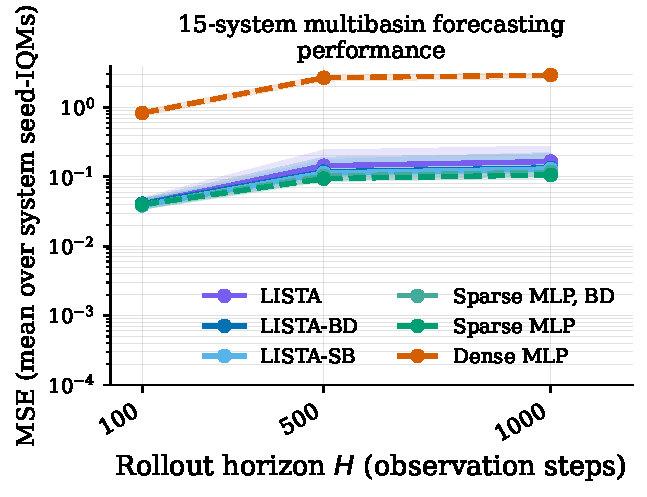
\includegraphics[width=\textwidth]{figures/neurips_paper_2026/fig_fixed17_horizon_curves.pdf}
\caption{Forecasting horizon trends on the \(15\)-system controlled benchmark. Lines show arithmetic means across all retained systems after summarizing finite seeds within each system by IQM; no system is trimmed. Bands show fixed-system seed-bootstrap 95\% intervals after system-wise log-relative normalization, anchored to the displayed all-system mean. They summarize finite-seed uncertainty for an equally weighted average system, not cross-system heterogeneity.}
\label{fig:forecasting_horizon_curves}
\end{figure}

\subsection{High-dimensional stress tests}
\label{sec:highdimensional_confirmations}

\begin{figure}[tbp]
\centering
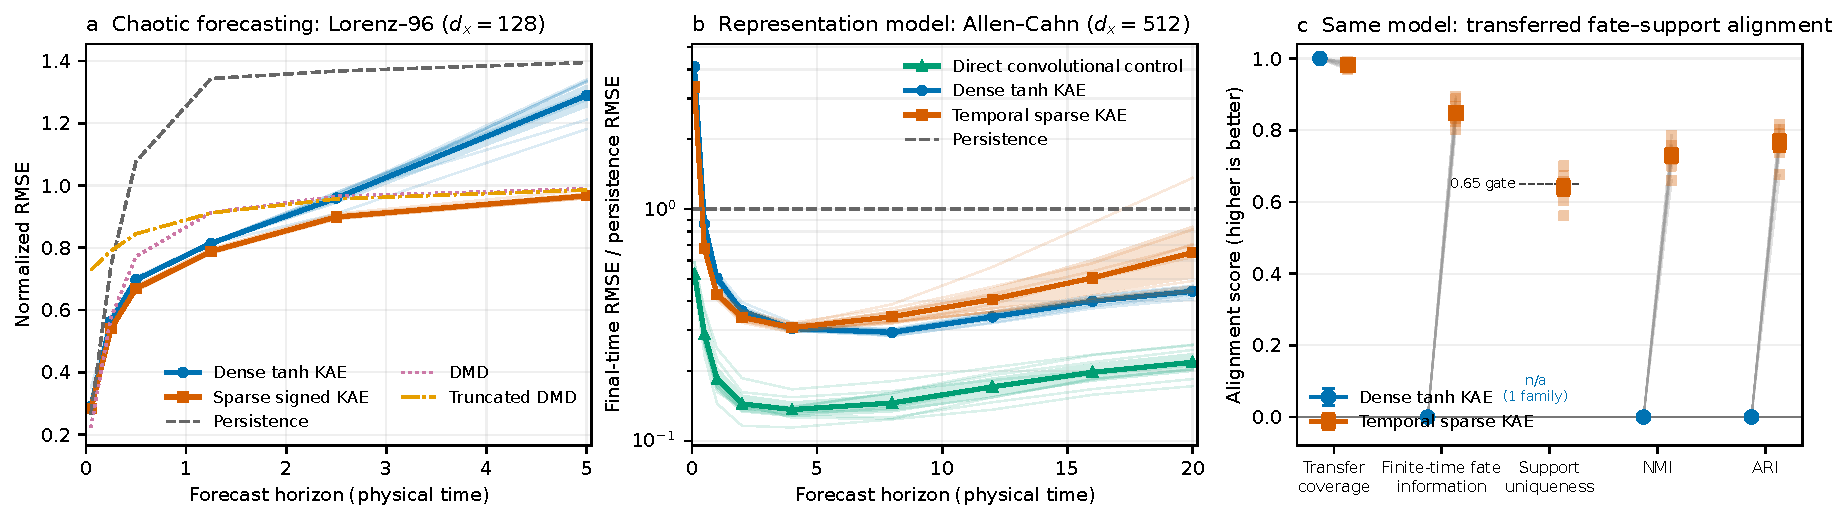
\includegraphics[width=\textwidth]{figures/neurips_paper_2026/fig_highdimensional_confirmation.pdf}
\caption{Separate high-dimensional evidence; faint lines or paired traces are individual model seeds and opaque marks show means with 95\% model-seed bootstrap intervals. \textbf{(a)} Fixed-data Lorenz--96 forecasting through physical time \(5\). \textbf{(b)} Final-time Allen--Cahn RMSE relative to persistence through physical time \(20\), on a logarithmic ordinate. \textbf{(c)} Final-state support transfer to a new-simulation-seed Allen--Cahn holdout. Panels (b,c) use the representation-focused temporal-support model, not the separate forecast-optimized model in \cref{fig:allen_cahn_global_k_forecast_optimized}. Finite-time fate information is \(1-H(B\mid F)/H(B)\), and support uniqueness is \(1-H(F\mid B)/H(F)\); the latter is \(0.641\), narrowly below its internally frozen \(0.65\) gate. The single-well slice was prospectively frozen for this new holdout after earlier mixed-domain fragmentation. Thresholded dense support yields one family and therefore zero support-family NMI and ARI; this does not test information in dense latent values.}
\label{fig:highdimensional_confirmation}
\end{figure}

\paragraph{Sparse forecasting survives a genuinely dense high-dimensional control.}
On fixed \(d_x=128\) Lorenz--96 data with \(d_z=512\), the signed-support KAE recipe reduces NRMSE relative to the exact-dense tanh KAE by \(6.30\%\) (95\% interval \([5.09\%,7.32\%]\)) at physical time \(2.5\) and \(24.87\%\) (\([22.98\%,26.51\%]\)) at time \(5\). It wins all ten paired seeds at both horizons; exact two-sided sign-flip tests followed by Holm correction give \(p=0.003906\) for each. Both rows use direct repeated-\(K\) rollout without re-encoding. Dense hidden layers use tanh, the latent output is linear, and sparsity, weight decay, transition regularization, and every zero-inducing module are absent; all ten audits pass and active density is \(0.9996\), versus \(0.4884\) for signed LISTA. This is a complete-recipe comparison: sign splitting mechanically permits at most one active coefficient per pair, and LISTA versus MLP parameterization and decoder normalization differ.
The time-5 endpoint is five times the 20-step training window, and sparse also has lower NRMSE than persistence, ordinary DMD, and rank-32 DMD at both declared long horizons.

\paragraph{PDE fate transfer in single-well-dominated fields.}
On the new \(d_x=512,d_z=2{,}048\) four-well Allen--Cahn test, the validation-fitted sign-split temporal-support family map has transfer coverage \(0.982\), ARI \(0.767\) (\([0.742,0.787]\)), NMI \(0.730\), and purity \(0.923\); thresholded dense support transfers one family and has ARI zero, which does not test information in dense latent values. Sparse wins all ten paired support-ARI comparisons (\(p=0.001953\)). Across all 256 trajectory final states, its normalized \(H(F\mid B)/H(F)=0.359\), or support-uniqueness score \(0.641\), misses the frozen \(0.65\) gate by \(0.009\) and its mean 10.8 families exceed the four finite-time fates. Both support families and modal-well fate labels are evaluated from the \(T=20\) final field; this is neither fate prediction from \(x_0\) nor trajectory-wide alignment. On the evaluation-only slice prospectively frozen for this new holdout after earlier mixed-domain fragmentation, whose final fields occupy their modal well over at least \(90\%\) of the grid, all ten model seeds yield exactly four families and perfect ARI, NMI, purity, and both conditional-entropy scores across 130/256 trajectories. Thus this single-well-dominated final-field slice has exactly one transferred family per finite-time modal-well fate; it does not prove geometric basin-interior membership. The remaining fragmentation is associated with spatially mixed, interface-rich final fields. This model has near-complete pre-split group activity and is not evidence that coefficient sparsity causes alignment: it improves over dense through physical time \(4\), but loses from time \(8\) onward. At time \(20\), direct, dense, and sign-support final RMSE relative to persistence are \(0.218\), \(0.442\), and \(0.649\).

\paragraph{A separate soft-thresholded sparse global model improves through-horizon PDE forecasting.}
With direct repeated-\(K\) rollout and no periodic re-encoding, the forecast-optimized soft-thresholded sparse recipe has mean field MSE \(0.04220\) versus \(0.04503\) for audited dense tanh through physical time \(16\), and \(0.04472\) versus \(0.04731\) through time \(20\). These are ratio-of-arm-means reductions of \(6.30\%\) and \(5.48\%\), each with 8/10 paired-seed wins and marginal paired-seed bootstrap intervals \([2.60\%,9.54\%]\) and \([1.75\%,8.76\%]\). Their MSE ratios to persistence are \(0.0958/0.1023\) at time 16 and \(0.0938/0.0993\) at time 20 for sparse/dense. Terminal reductions are smaller---\(2.38\%\) and \(3.22\%\)---with intervals crossing zero. Both arms have the same trainable tensor shapes/count and shared convolutional, decoder, and \(K\) backbone, \(12{,}698{,}690\) trainable parameter entries, and \(8{,}504{,}386\) effective forward-path parameters; the joint treatment is soft-thresholding at \(0.15\) plus an \(L_1\) weight of \(0.01\). The internally frozen rule required all four through-horizon and terminal cells to pass; it failed, and the conditional holdout was not generated or opened. We subsequently froze the H200 through-horizon endpoint and crossed the same 20 checkpoints, without retraining or reselection, with three prospectively generated 256-trajectory datasets. Sparse/dense MSE is \(0.04616/0.04903\), a \(5.86\%\) full-trajectory mean reduction with 8/10 paired-seed wins, a paired-seed bootstrap interval \([2.40\%,9.21\%]\), exact one-sided sign-flip \(p=0.00879\), and positive effects of \(4.68\%/5.88\%/7.03\%\) on the three datasets. A frozen secondary translation on these exact forecasts finds favorable H200 cumulative direction on all seven phase/interface/energy metrics; pixel phase, well-area, interface, full-energy, and gradient-energy errors fall by \(4.61\%/6.07\%/2.25\%/6.20\%/8.58\%\) and survive seven-way Holm correction, while modal accuracy and potential-energy error are positive but nonsignificant. This outcome-aware same-checkpoint evidence establishes new-initial-condition robustness and broad physical concordance in the same condition, not independent retraining replication, a repair of the original four-cell gate, terminal superiority, or cross-condition physics generalization. The model is soft-thresholded with mean evaluated latent near-zero fraction \(0.434\) at \(|z|\le10^{-3}\), versus \(0.0025\) for dense, but it is trained separately from the temporal-support model, so no alignment-to-forecast mediation or single-component attribution is claimed.

\begin{figure}[tbp]
\centering
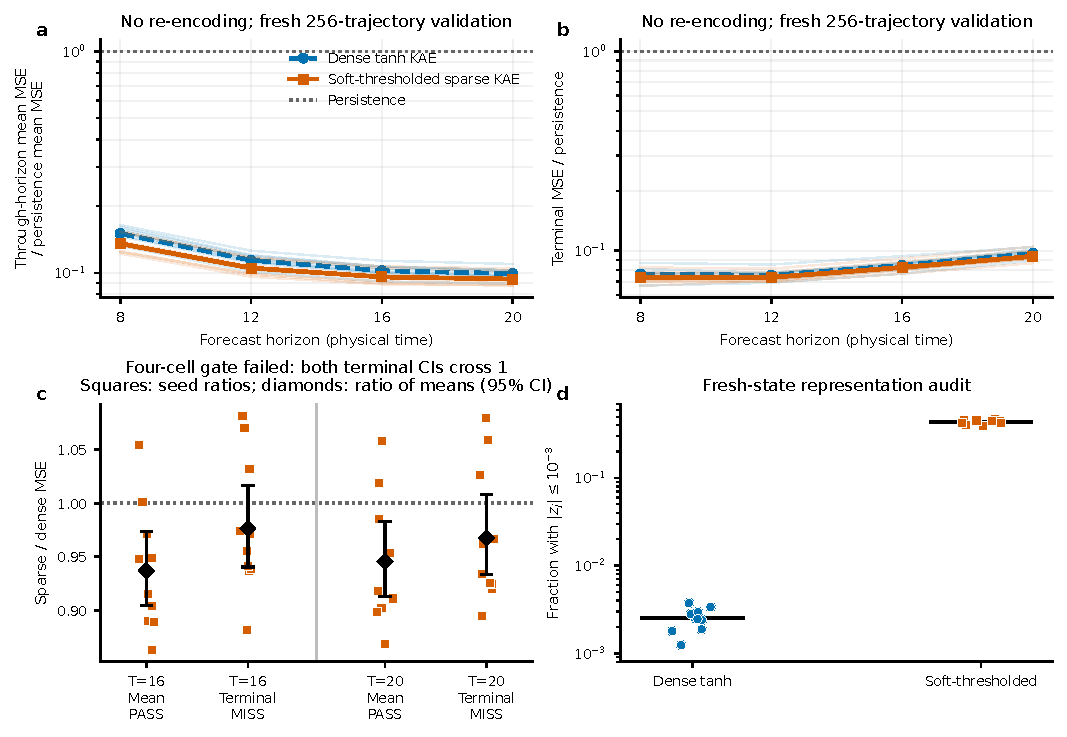
\includegraphics[width=\textwidth]{figures/neurips_paper_2026/fig_allen_cahn_global_k_forecast_optimized.pdf}
\caption{Separate forecast-optimized Allen--Cahn comparison on 256 fresh validation trajectories. Both KAEs use direct rollout without re-encoding. Panels report mean and terminal field MSE relative to persistence, all four frozen H160/H200 mean and terminal cells, and fresh-state near-zero fractions. In panel (c), orange squares are individual paired-seed sparse/dense ratios; black diamonds are ratios of arm means with marginal paired-seed bootstrap intervals, so a diamond need not center the seed ratios. The through-horizon sparse effects are positive, while both terminal marginal intervals include one. H200 terminal has a \(3.22\%\) reduction and 7/10 wins, below the frozen \(5\%\) and 8/10 criteria, so the four-cell gate fails.}
\label{fig:allen_cahn_global_k_forecast_optimized}
\end{figure}

\begin{figure}[tbp]
\centering
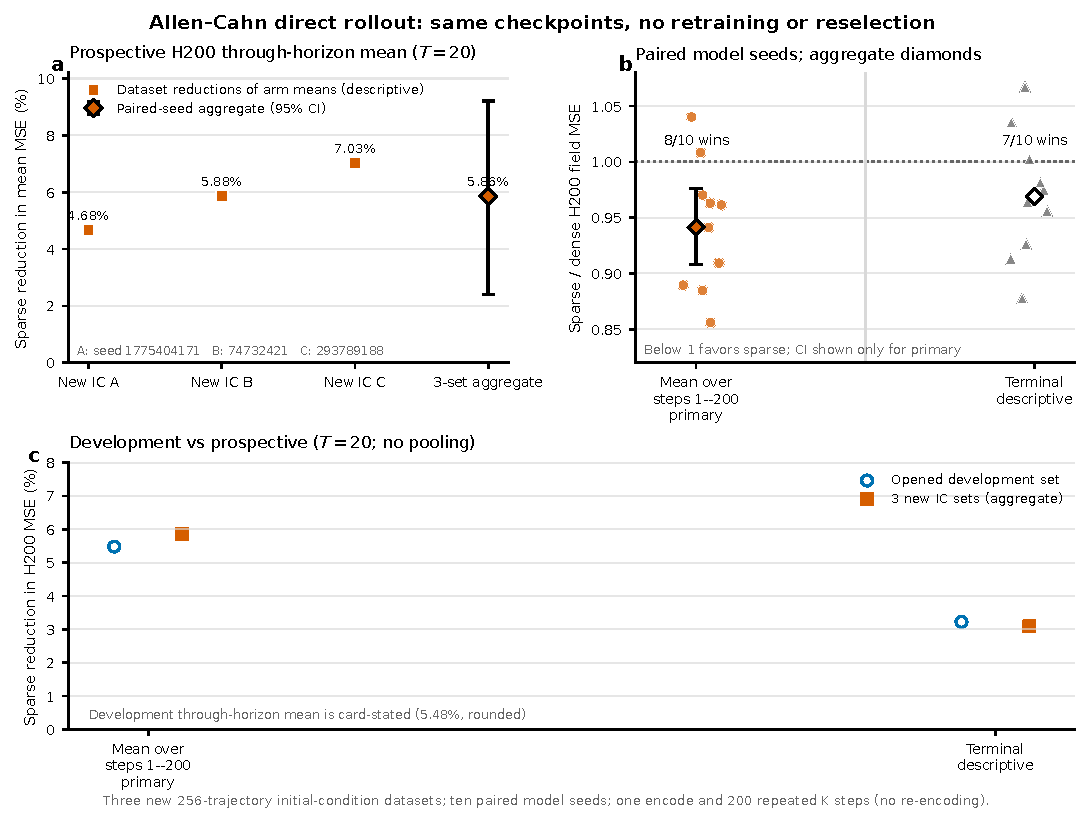
\includegraphics[width=\textwidth]{figures/neurips_paper_2026/fig_allen_cahn_new_ic_replication.pdf}
\caption{Same-checkpoint Allen--Cahn new-initial-condition robustness check at H200 (physical time 20). The endpoint was frozen after the original four-cell gate failed. The three prospectively generated dataset effects are descriptive; inference averages datasets within paired model seed. Opened development and new-IC results are displayed separately and never pooled. Checkpoints were neither retrained nor reselected.}
\label{fig:allen_cahn_new_ic_replication}
\end{figure}

\paragraph{The same checkpoints do not validate support-selected Allen--Cahn local laws.}
An internally metric-blind audit used score-initial supports only, locked every
projector before future encoding, and rolled out the same global \(K\) without
re-encoding. Provenance, information-firewall, and exact initial-capture
checks pass, but the sparse masks remain broad (mean active fraction \(0.696\),
or \(1{,}425/2{,}048\) coordinates) and every one of ten seeds yields a single
training-fitted support family. Thus zero seeds meet the predeclared
two-family gate, making family-specific signature and routing estimands
undefined. Exact-support raw-\(K\) leakage is \(3.29\) and \(3.25\) times
the coordinate-permutation null at H160/H200, the global-\(K\)-over-identity
residual is \(1.052>1\), and every matched-dense specificity family fails; the
predeclared \(x_0\)-support operationalization therefore fails on these
checkpoints. Repeated fixed-support
sparse forecasts nevertheless have \(5.81\%\) and \(6.27\%\) lower mean field
MSE than dense full forecasts (8/10 wins; intervals
\([1.58\%,9.55\%]\) and \([2.20\%,9.87\%]\)). This is a same-checkpoint,
same-score-set decomposition of the preceding forecast comparison, not an
independent validation: the result supports the bounded sparse-versus-dense
forecast statement but not support-mediated prediction, approximate invariant
coordinate subspaces, or distinct local laws. The conditional new-dataset
mechanism bridge was ineligible and was not launched.

\paragraph{Support projections reduce one-step leakage without establishing invariance.}
In a separate held-out one-step diagnostic across all 15 controlled systems
and three seeds, a no-next-state guard emitted by the evaluator before
execution has support-projected leakage \(0.0047\), versus \(0.2065\) under a
sign-pair-preserving coordinate-permutation null. Leakage normalized by actual
\(K-I\) change is \(0.338\) versus \(0.783\). Whole-matrix Frobenius leakage
is \(0.0538\) versus \(0.2080\), or \(0.554\) versus \(0.783\) after the same
change normalization; every system favors the observed masks on all four
diagnostics. Their ratios are numerically close to the internally frozen
future-persistent primary. The guard adds only 0.96 percentage points because
persistence is high, so this shows robustness on a highly persistent sample;
it neither removes the future-conditioning concern broadly nor tests
boundary-heavy switching. Observed support-projected one-step leakage is lower than under
matched permutations, but does not establish invariant coordinate subspaces or distinct local laws:
operator differentiation is null-like (ratio \(0.993\)) and fails.
The test remains two-dimensional and latent rather than decoded or multistep.
A triggered zero-weight-decay dense tanh control uses the same physical states and per-state sparse cardinalities: activity observed/null is \(0.022\) sparse
versus \(0.567\) dense (ratio \(0.039\)), while restricted-residual observed/null
is \(0.053\) versus \(0.486\) (ratio \(0.108\)); all 14 common eligible systems
favor sparse. This supports complete-recipe
specificity relative to matched dense top-\(k\) coordinates, not a
sparsity-only causal effect; see \cref{app:global_k_support_closure}.


\begin{figure}[tbp!]
\centering
\begin{subfigure}[t]{0.47\linewidth}
  \vspace{0pt}
  \centering
  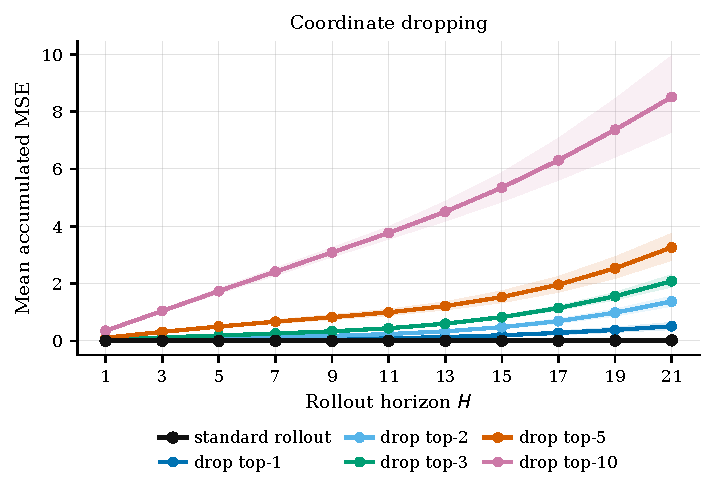
\includegraphics[width=\linewidth]{figures/neurips_paper_2026/fig_support_coordinate_dropping_accumulated_mse.pdf}
  \caption{Dropping the largest active coordinates.}
  \label{fig:support_coordinate_dropping}
\end{subfigure}
\hfill
\begin{subfigure}[t]{0.47\linewidth}
  \vspace{0pt}
  \centering
  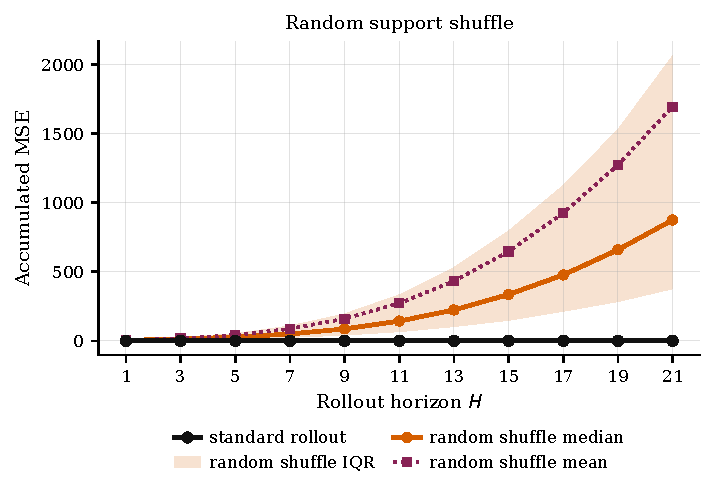
\includegraphics[width=\linewidth]{figures/neurips_paper_2026/fig_support_coordinate_random_shuffle_accumulated_mse.pdf}
  \caption{Moving active values to inactive coordinates.}
  \label{fig:support_coordinate_random}
\end{subfigure}
\caption{Descriptive support-coordinate interventions for one Local-linear gates LISTA checkpoint (seed \(0\)). \textbf{(a)} The standard rollout is compared with cumulative dropping of the largest active coordinates of the initial sparse code; bands are bootstrap 95\% intervals over \(100\) starts. \textbf{(b)} Active values are reassigned to random inactive coordinates; the band is the interquartile range of the pooled \(2{,}000\) dependent point--shuffle outcomes (\(100\) starts times \(20\) shuffles) at each horizon. No confirmatory test is attached.}
\label{fig:support_coordinate_interventions}
\end{figure}

\begin{wrapfigure}[25]{R}{0.4\linewidth}
\vspace{-1em}
\centering
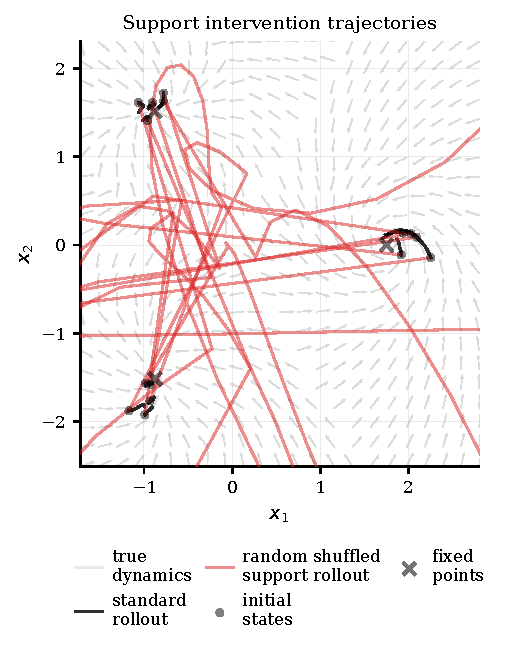
\includegraphics[width=\linewidth]{figures/neurips_paper_2026/fig_support_coordinate_trajectories_random_support_19.pdf}
\caption{Randomly shuffled support trajectories (red) and standard rollouts (black) for the same representative checkpoint.}
\label{fig:support_coordinate_trajectories}
\end{wrapfigure}



\paragraph{Representative support-coordinate intervention.} As a scoped mechanism diagnostic, we perturb the initial active set of one Local-linear gates LISTA checkpoint at seed \(0\) and evaluate 21-step forecasts. The evaluator first restricts candidates to the tie-inclusive high center-margin slice whose native label remains equal to its initial label throughout the \(21\)-step true future. It balances the retained \(100\) starts across the three native labels (\(34/33/33\)); coordinate dropping and random support use exactly the same starts. The interventions are:
\begin{enumerate}
    \item \textbf{Coordinate dropping:} Force the coordinates of $z$ with the $k\in\{1,2,3,5,10\}$ largest magnitude coefficients to zero before forecasting.
    \item \textbf{Random support:} the active coefficient values are preserved, but reassigned to randomly chosen inactive latent coordinates.
\end{enumerate}

At \(H=21\), the standard rollout has mean accumulated MSE \(0.0158\). Dropping \(k=1,2,3,5,\) and \(10\) leading coordinates raises this to \(0.508\), \(1.37\), \(2.08\), \(3.26\), and \(8.51\), respectively; random support shuffling is also destructive in \cref{fig:support_coordinate_interventions,app:support_coordinate_interventions}. This is descriptive evidence that this checkpoint uses coordinate identity. Because it covers one system, model, and seed and has no confirmatory test, it does not establish a general causal effect across architectures or systems.




\subsection{Support-basin alignment experiments}


This post-hoc experiment examines whether sparse support families fit after training are associated with evaluation-only native or proxy basin labels.
For the two gated environments, the evaluator uses native labels and centers. For the \(13\) catalog environments, it rolls the \(128\) trajectory endpoints forward \(5{,}000\) steps, clusters the converged endpoints into the known benchmark count by deterministic \(k\)-means, and labels every state by its nearest estimated center. Fourteen systems realize at least two observed labels; the Triple-well Duffing proxy assigns all \(16{,}512\) states to one estimated center. Native and proxy labels and centers do not enter model training or support-family formation. The known count enters structured-transition block sizing as disclosed above, but its use here is post-hoc center estimation rather than a feature in the learned support or route.


For a state \(x\), let \(d_1(x)\) and \(d_2(x)\) be its distances to the nearest and second-nearest native or estimated center. We call \(d_2(x)-d_1(x)\) the \textit{center-margin proxy}. A large value indicates separation under this nearest-center construction; it need not equal distance to a true basin boundary or separatrix, especially when basin geometry is not Voronoi.
The diagnostic first fits \(F_{\rm abs}^{\rm align}\) using the absolute threshold \(10^{-3}\) and Jaccard threshold \(0.50\) over all states in each evaluation trajectory collection. It then retains states at or above the within-label \(75\)th percentile of center margin, including all ties, and scores the already fitted partition against label \(B\). This threshold does not resample labels to equal sizes and does not guarantee that exactly \(25\%\) of each label is retained. Conditional entropy \(H(B\mid F_{\rm abs}^{\rm align})\), computed with natural logarithms and reported in nats, is the main metric; the number of family IDs observed on the high-margin slice is a descriptive companion. Most system--seed slices contain \(4{,}129\)--\(7{,}167\) states. Triple-well Duffing retains all \(16{,}512\) because its center margins tie, but its one-label proxy makes \(H(B\mid F)=0\) for every model and therefore cannot measure alignment. Primary point estimates and tests use the \(14\) systems with at least two observed labels; all raw Duffing rows remain in the evidence packet and an all-\(15\)-system sensitivity sidecar. Because the scored states belong to the same evaluation trajectory collection used both to estimate catalog-system centers and to fit the partition, this measures transductive alignment to native or proxy labels, not generalization of a frozen family codebook.

\begin{table}[tbp]
\centering
\caption{Transductive basin-support diagnostics on the \(14\) controlled systems whose frozen evaluation assignment realizes at least two labels. \(F_{\rm abs}\) is fitted over all states in each evaluation trajectory collection with absolute threshold \(10^{-3}\) and Jaccard threshold \(0.50\), then scored at or above the within-label \(75\)th center-margin percentile, retaining ties. Labels and centers are native for two gated systems and nearest-center proxies from deterministic endpoint clustering at the known benchmark count for the catalog systems. They define and score the subset but do not enter family formation or equalize label counts. \(H(B\mid F_{\rm abs})\) uses natural logarithms and is reported in nats. \(\overline{|F_{\rm abs}|}\) counts family IDs observed on the scored slice and uses ordinary seed means. Triple-well Duffing's proxy realizes one label, so its identically zero entropy is excluded from primary aggregates; its raw rows and all-\(15\)-system sensitivity are retained. Superscripts mark Wilcoxon/Holm tests against Dense MLP (\(\ast\), \(p<0.05\)); all displayed stars pass on all \(14/14\) eligible systems. \textbf{Bold} marks the best directional entry.}
\label{tab:controlled_alignment}
\label{tab:support_diagnostics_main}
{\setlength{\tabcolsep}{4pt}
\resizebox{0.62\textwidth}{!}{\begin{tabular}[t]{@{}l rr@{}}
\toprule
& \multicolumn{2}{c}{Tie-inclusive high-margin slice, 14 systems} \\
\cmidrule(l){2-3}
Model & $H(B\!\mid\!F_{\rm abs})\,[\mathrm{nats}]\downarrow$ & $\overline{|F_{\rm abs}^{\rm obs}|}$ \\
\midrule
LISTA & ${\mathbf{0.138}}^{\ast}$ & $\mathbf{3.6}$ \\
LISTA-BD & ${0.173}^{\ast}$ & $3.5$ \\
LISTA-SB & ${0.168}^{\ast}$ & $3.5$ \\
Sparse MLP, BD & ${0.386}^{\ast}$ & $3.0$ \\
Sparse MLP & ${0.244}^{\ast}$ & $3.3$ \\
\midrule
Dense MLP & $1.37$\,\emph{[baseline]} & $1.0$\,\emph{[baseline]} \\
\bottomrule
\end{tabular}
}}
\end{table}

\paragraph{LISTA families align with evaluation labels on high center-margin states.}
In \cref{tab:controlled_alignment}, LISTA has the lowest primary transductive conditional entropy, \(0.138\) nats, compared with \(1.37\) nats for Dense MLP. The other sparse rows lie between these values. The scored high-margin slice contains \(3.6\) LISTA family IDs on average, compared with a mean/median of \(4.29/4\) represented labels across the \(14\) systems, whereas Dense MLP exposes one family ID on average. These are ordinary seed means of observed slice counts, not total partition sizes. All-\(15\)-system sensitivity values are \(0.129\) and \(1.28\) nats for LISTA and Dense MLP, respectively; including the uninformative zero therefore reduces both estimates. A historical 1,345-run sweep is locally stable around Jaccard \(0.4\)--\(0.6\), but \(0.2\) merges families and \(0.9\) fragments to about \(33.8\) families while driving entropy near zero, so family count must accompany entropy. Alignment tests pass after correction on all \(14/14\) eligible systems. This is evidence of post-hoc alignment to this evaluation label construction; it does not show that the center margin measures true boundary distance, that a frozen family map discovers new basins out of sample, or that every family corresponds one-to-one with a basin.

\subsection{Support-family local linearizations}
\label{sec:fabs_local_linearizations}

We next test a separate, controlled routing protocol. The staged model and global-\(K\) baseline use the same LISTA architecture and total \(200{,}000\)-step budget. Stage one trains the encoder, decoder, and shared \(K\) for \(100{,}000\) steps. We then freeze all three and fit \(F_{\rm abs}^{\rm route}\) on a nominal \(512\)-row packet from the training distribution. The source implementation generated one batch of \(256\) unique trajectories and repeated it exactly, so this packet contains \(256\), not \(512\), unique trajectories. Each trajectory has \(192\) transitions and \(193\) states. The greedy \(10^{-3}\)-threshold, Jaccard-\(0.40\) family merge sees all \(193\) state supports, including terminal states; map counts, source centers, and direct mask keys then use the first \(192\) source states. This gives \(98{,}816\) nominal supports for clustering, \(98{,}304\) nominal source transitions, and \(49{,}152\) unique source transitions. Families with at least one source transition receive affine maps trained for another \(100{,}000\) steps.

For support family \(f\), let \(\bar z_f\) be the mean source latent assigned to that family. The route-local update is
\begin{equation}
  T_f(z)=d_f+K_f(z-\bar z_f),
  \label{eq:fabs_local_affine}
\end{equation}
where \(K_f\) is initialized from the frozen global matrix and the learned intercept \(d_f\) is initialized to \(K\bar z_f\). The runtime representative of each merged family is its modal source-state support mask. Before every latent transition, the model recomputes the current latent's absolute support and routes that step against the frozen representatives; an unassigned route falls back to the frozen global \(K\). Scheduled periodic events instead decode and re-encode the predicted state, refreshing the latent before the next step's route. Thus routing occurs every latent step even when re-encoding is less frequent. Neither construction nor rollout uses basin labels, counts, attractor identities, or trajectory assignments. For each horizon, both staged and global rows are reported at their evaluation-set oracle cadence from \(m\in\{1,2,5,10,20,25,50,100\}\).

Checkpoint selection is not matched. The staged selector scores exactly \(200\) candidates---steps \(100{,}500,101{,}000,\ldots,199{,}500\), plus \(199{,}999\)---on \(32\) fixed starts at seed offset \(12{,}345\). For each candidate, it minimizes the finite-prefix, state-summed squared error independently across the cadence grid at H100, H500, and H1000, averages those three minima, and replaces the incumbent only on a strict improvement. Final reporting uses \(100\) starts at the same seed offset, so the selector starts are exactly the first \(32\) reported starts (32\% overlap). By contrast, the global baseline uses its standard \(16\)-start, seed-offset-\(999{,}999\), every-step-re-encoded H200 final-error selector, which has no overlap with the reported starts. Thus architecture and optimization budget are shared, but the staged comparison is descriptive and optimistic rather than a clean held-out checkpoint comparison.

Across the \(15\) controlled systems and \(15\) seeds, the routed model has lower MSE on \(199/225\), \(192/225\), and \(189/225\) system--seed pairs at H100, H500, and H1000; median local/global ratios are \(0.355\), \(0.312\), and \(0.328\). Matched H1000 random-count, latent-k-means, and oracle-basin routing packets also improve on global \(K\), with median ratios \(0.451/0.341/0.366\) and \(185/196/195\) wins, respectively; local maps help this staged artifact, but support identity is not uniquely implicated. These \(225\) pairs are nested within \(15\) systems and are reported descriptively, without treating them as independent units or attaching confirmatory inference. Selector overlap and asymmetry preclude a clean causal or held-out routing comparison.

\begin{table}[tbp]
\centering
\caption{Staged \(F_{\rm abs}^{\rm route}\)-routed local affine forecasting on the controlled benchmark. The same-architecture, same-budget global-\(K\) LISTA baseline has \(d_z=256\), but checkpoint selection is asymmetric: the staged selector overlaps the first \(32/100\) reported starts, whereas the global selector uses distinct starts. Both rows also select cadence on the reported starts over the same fixed grid. Pair counts are descriptive nested system--seed outcomes; the last column counts pairs won by the routed model at H100, H500, and H1000 simultaneously. Lower MSEs and ratios are better.}
\label{tab:fabs_local_k_forecasting}
{\setlength{\tabcolsep}{4pt}
\resizebox{0.92\textwidth}{!}{\begin{tabular}{lcccc}
\toprule
Metric & H100 & H500 & H1000 & All three horizons \\
\midrule
Paired local wins & $199/225$ & $192/225$ & $189/225$ & $180/225$ \\
Mean MSE, \(F_{\rm abs}^{\rm route}\)-local/global & $0.0128/0.0229$ & $0.0347/0.0623$ & $0.0403/0.0706$ & -- \\
Median local/global MSE ratio & $0.355$ & $0.312$ & $0.328$ & -- \\
Geometric local/global MSE ratio & $0.252$ & $0.180$ & $0.174$ & -- \\
\bottomrule
\end{tabular}
}}
\end{table}

\section{Discussion}
\label{sec:discussion}

The evidence supports three bounded claims. Sparse-latent KAE recipes have lower reported aggregate error than the Dense MLP rows on the controlled benchmark; direct-rollout Lorenz--96 and forecast-optimized Allen--Cahn comparisons extend this to high dimension. The historical Dysts comparison is not evidence because its KAE cache cadence was mislabeled, and its corrected rerun remains pending. The Allen H200 through-horizon advantage persists with the same checkpoints across three new initial-condition datasets, and a subsequently frozen outcome-aware audit of seven correlated state-derived metrics shows broad phase/interface/energy concordance, while independent retraining replication, terminal superiority, PDE-law validation, and cross-condition generalization remain unsupported. On high center-margin controlled-benchmark states, LISTA families have low transductive conditional entropy with evaluation-only native or nearest-center-proxy labels. A different Allen--Cahn temporal-support model transfers a validation-fitted map to unseen PDE trajectories: across all trajectory final states, \(T=20\) supports are informative about the \(T=20\) modal-well fate, and the single-well-dominated final-field slice prospectively frozen for the new holdout after earlier mixed-domain fragmentation has exactly one transferred family per fate for every seed, although the stricter all-trajectory final-state uniqueness gate narrowly fails. In a separate staged artifact, training-distribution support families route local affine maps and have descriptively lower controlled-forecasting error than a same-budget global-\(K\) LISTA model, subject to selector leakage and asymmetry. These forecasting, alignment, and routing results arise from different recipes and do not identify a representation-to-forecast causal chain.

These results motivate a hybrid interpretation in which coefficient values carry continuous predictive coordinates and active-coordinate identities provide an inspectable regime key. An exact direct-sum affine lift shows that one matrix can contain several support-selected local laws in principle, without showing that learning discovers them. The held-out controlled diagnostic finds lower support-conditioned one-step leakage than matched coordinate-permutation controls for one unchanged \(K\); an evaluator-emitted all-current guard gives similar ratios, but adds only 0.96 percentage points on a highly persistent sample. It therefore does not resolve boundary-switching behavior or remove the future-conditioning concern generally. Its operator-differentiation gate still fails, although the triggered exact-dense control establishes complete-recipe specificity relative to cardinality-matched dense coordinates. A final frozen recursive residual-routing diagnostic was invalid at its frozen validity tier and directionally unadjudicated after a nonfinite payload value (\texttt{inf}) prevented completion of the exact-ten packet; no partial outcome was inspected. We do not claim an exact global finite-dimensional linearization, a one-to-one support--basin theorem, supervised-quality basin recovery, distinct support-local laws, or that representation quality mediates forecasting. Periodic decode--encode is an autonomous nonlinear composite predictor, not a guaranteed mathematical projection; the best-periodic values in the submitted binary PDF are not uniformly pure \(K^h\) and were selected over re-encoding cadences on report trajectories. The separate no-re-encoding comparisons more directly test the KAE objective. The staged result is specific to its fitted partition and affine-map recipe and does not establish deployment-ready routing.

Several protocol limitations constrain the conclusions. First, all reported best-periodic values choose cadence separately at each horizon on the same test trajectories; validation-frozen cadence selection is needed for deployment-style estimates. The MSE reducer also omits nonfinite steps, so finite prefixes can make divergent rollouts appear better than a strict full-horizon failure rule. Every ordinary controlled row and both stages of the staged model also cycle only eight fixed training batches per seed because the maintained child-seed streams are not advanced, substantially limiting training-data diversity. Second, the controlled alignment partition is fitted over the same evaluation trajectory collection that contains the high center-margin states used for scoring. For \(13\) systems, the same collection also supplies the endpoints used to estimate centers, and the known benchmark count enters that evaluation-only construction. The resulting nearest-center labels and \(d_2-d_1\) margin are proxies and need not recover true basin geometry or boundary distance. The Allen--Cahn transfer and forecasting packets remove this particular fit--score overlap, but remain one synthetic PDE condition and are not evidence on empirical real-world data. Validation fate metrics selected the transfer packet's T20 scope, Jaccard-0.40 rule, temporal weight, and advancement of the fixed ten-seed roster; its all-trajectory final-state uniqueness gate misses by \(0.009\). The original forecast packet fails its four-cell gate and was selected after a three-seed/four-recipe screen; the later H200 same-checkpoint check freezes an outcome-aware endpoint and only changes initial-condition datasets. Neither establishes population generalization over retraining, PDE parameters, grids, or systems.

Third, the \(225\) staged system--seed pairs are nested within \(15\) systems and receive no confirmatory system-level inference. Its route-fit packet contains only \(256\) unique trajectories despite \(512\) configured rows, and its checkpoint selector reuses \(32\%\) of the reported starts while the global baseline uses a different selector. The result should be rerun from a newly versioned 512-unique route fit with disjoint, common checkpoint-validation starts and a validation-frozen cadence before making a general routing claim. Cross-family attribution is also limited because LISTA decoders are atom-normalized whereas MLP decoders are not, and the structured-transition rows use a known controlled-benchmark basin count solely to size their blocks. The corrected Dysts comparison removes the historical LISTA-SB depth confound by using one learned refinement in all three LISTA rows and uses a tanh, zero-sparsity dense baseline. A separate historical 15-seed \(d_z=1{,}024\) stress test on fixed eight-basin competitive Lotka--Volterra, Hopfield \(N=P=16\), and Kuramoto \(N=16\) favored tanh Dense MLP over every sparse/LISTA recipe at H100/H500/H1000 under evaluation-selected best-periodic cadence; it is a required negative recipe comparison, not a sparsity-only ablation. Finally, standalone controls use three seeds and independently generated trajectories, and the coordinate intervention uses only one Local-linear gates LISTA checkpoint at seed \(0\). These comparisons remain descriptive.

The immediate priorities are therefore to complete the corrected all-row Dysts rerun; finish the paired Allen--Cahn two-versus-three-refinement study; stop outcome-adaptive work on the opened controlled mechanism condition; freeze forecasting cadence on validation data with strict finiteness accounting; and test frozen recipes prospectively across new physical conditions.

\appendix

\section{Additional experimental details}
\label{app:experimental_details}

This appendix records the paper-facing experimental protocol. The main experiments ask whether sparse Koopman autoencoders learn useful latent supports without basin supervision. The model is never given basin labels, basin counts, or trajectory-to-basin assignments when training the encoder, decoder, latent transition, support rules, or periodic rollouts. Benchmark basin metadata is used only after training to define evaluation slices, construct controlled diagnostic interventions, and score support--basin agreement. The only training-time exception is architectural: the block-diagonal and soft-block transition diagnostics use benchmark metadata to set the fixed number of transition groups, but they still do not receive trajectory labels or support labels.

\paragraph{Benchmarks.}
The controlled benchmark contains \(15\) two-dimensional multibasin systems, listed with their equations and attractor metadata in \cref{app:fixed17_inventory}. These systems are integrated to produce stored observation sequences; the learner observes only stored states, not vector fields, integration substeps, basin labels, or basin assignments. The external forecasting stress test uses the \(10\) three-dimensional Dysts \(dt{\times}30\) systems listed in \cref{app:dysts_inventory_full}. For Dysts, stored observations are generated at \(30\) times each system's native integration interval and coordinates are standardized after trajectory generation.

\paragraph{Model rows.}
The six model rows in \cref{tab:forecasting_main,tab:fixed17_alignment} are LISTA, LISTA--BD, LISTA--SB, Sparse MLP, Sparse MLP--BD, and Dense MLP. All use latent dimension \(d_z=256\). LISTA rows use shrinkage to produce exact zeros; MLP sparse rows use the sparsity penalty in \cref{eq:loss_latent_terms}; Dense MLP removes the intended sparsity mechanism and sets the sparsity coefficient to zero. The BD rows use a block-diagonal latent transition. The SB row keeps a dense transition but adds an off-block penalty. All rows use a linear decoder dictionary as the state decoder. The controlled multibasin LISTA rows use threshold scale \(\alpha=0.15\), two shrinkage-refinement loops, and a sign-split final operation. The Dysts \(dt{\times}30\) LISTA rows use the same threshold scale with one refinement loop and a ReLU final operation. MLP encoders use two hidden layers of width \(64\); Dense MLP uses a tanh encoder without the sparse output gate.

\paragraph{Controlled multibasin training.}
For every controlled system, each model row is trained for seeds \(0,\ldots,14\). Training uses rollout length \(L=8\) windows, meaning \(9\) adjacent stored states per window, for \(200{,}000\) optimization steps with minibatches of \(256\) windows. The optimizer is AdamW. Encoder and decoder parameters use learning rate \(5{\times}10^{-5}\), the latent transition uses learning rate \(5{\times}10^{-6}\), and non-transition parameters use weight decay \(10^{-4}\). In \cref{eq:training_objective}, the loss weights are \(\lambda_{\rm pred}=1\), \(\lambda_{\rm rec}=0.03\), \(\lambda_{\rm lin}=1\), and \(\lambda_{\rm sp}=3{\times}10^{-3}\) for sparse rows; Dense MLP uses \(\lambda_{\rm sp}=0\). Soft-block rows add the off-block \(L_1\) transition penalty with weight \(10^{-4}\).

All controlled rows use the same label-free boundary-emphasized reset distribution. Before training, \(4096\) candidate initial states are probed for \(32\) steps. Candidates are scored by short-horizon perturbation sensitivity and residual late-rollout motion, and the top \(1024\) states are retained. The scoring probe uses four perturbations, perturbation scale \(0.04\), a late-transient window of \(8\) steps, and transient weight \(0.5\). Half of training windows start from this retained pool with jitter scale \(0.25\). The retained pool is intended to expose boundary-adjacent and transient regions that would otherwise be rare under ordinary resets; it is built without basin labels.

\paragraph{Dysts \(dt{\times}30\) training.}
Dysts rows are trained for the same seeds, \(0,\ldots,14\), with latent dimension \(d_z=256\), minibatches of \(256\), rollout length \(L=10\) windows, and \(100{,}000\) optimization steps. Dysts trajectories come from deterministic native caches with \(200\) cached trajectories, \(30{,}000\) stored observations per trajectory, and a \(2{,}000\)-step warm-up. The first cached trajectory starts from the Dysts default initial condition; remaining trajectories perturb that state with Gaussian noise at scale \(0.2\) times the coordinate-wise Dysts standard deviation. Train, validation, and test caches use separate deterministic namespaces, so held-out test windows are disjoint from training windows and reusable across model seeds. LISTA rows use the controlled-benchmark learning rates. MLP rows use learning rates \(10^{-4}\) for encoder/decoder parameters and \(10^{-5}\) for the latent transition. Sparse Dysts rows use \(\lambda_{\rm sp}=6{\times}10^{-3}\), while Dense MLP uses \(\lambda_{\rm sp}=0\).

\paragraph{Checkpoint selection.}
Checkpoint selection is fixed before test evaluation. Every \(500\) optimization steps, and again at the final step, the current model is rolled out for \(200\) stored steps from \(16\) fixed held-out initial states using every-step re-encoding. The checkpoint with the lowest final validation error under this proxy is used for reported evaluations. Final tables aggregate completed seeds; they do not select the best seed.

\paragraph{Training recipe selection.}
Exploratory sweeps varied LISTA depth, shrinkage scale, sparsity coefficient, sign-split encodings, transition structure, and MLP sparsity controls. These sweeps used shorter budgets or broader system lists and are not pooled with the final evidence. The paper-facing protocol is the fixed recipe in this appendix: \(15\) seeds per retained system, the training budgets above, held-out evaluation splits, and the statistical units in \cref{app:statistical_testing}.

\paragraph{Forecasting experiments.}
Forecasting is evaluated on held-out trajectories at the stored observation cadence. A horizon \(h\) always means \(h\) stored observation steps, not a common physical time across systems. The no-reencoding rollout applies the learned latent transition for the full horizon before decoding. The periodic rollout advances the model's own predicted latent state, decodes the predicted state at a fixed period \(m\), and re-encodes that predicted state; it never uses the true future state. Controlled multibasin forecasting uses \(100\) held-out initial conditions for each system and seed and reports the best score over the fixed period grid \(m\in\{10,25,50,100\}\). Dysts long-horizon forecasting uses \(100\) held-out test-cache windows for each system and seed and reports the best score over \(m\in\{10,25,50,100,150,200\}\). These grids are fixed before aggregation and are not tuned separately for each test trajectory.

\paragraph{Support--basin alignment.}
Support alignment is computed after training from held-out controlled-system states. For each state \(x\), the basin-depth margin is the distance to the second-nearest benchmark attractor center minus the distance to the nearest attractor center. Within each represented benchmark basin, the evaluator keeps the top quartile of held-out states by this margin. This per-basin deep slice uses ground-truth geometry only to define the evaluation population. It is the clean slice for testing basin-support alignment because boundary states can legitimately have unstable or mixed supports.

On this slice, the evaluator encodes states and constructs \(S_{\rm abs}(x)=\{i:|z_i|>10^{-3}\}\). Exact Boolean masks are grouped into \(F_{\rm abs}\) support families by the deterministic greedy Jaccard rule in \cref{sec:method_supports,app:support_definitions} with threshold \(0.5\). The main directional metric is \(H(B\mid F_{\rm abs})\), where \(B\) is the withheld benchmark basin label; lower values mean that knowing the learned support family leaves less uncertainty about basin identity. The companion count \(\overline{|F_{\rm abs}|}\) is descriptive and is interpreted relative to the number of represented basins, not as a monotone score to maximize.

\paragraph{Wrong-support functional diagnostic.}
The cross-system wrong-support diagnostic asks whether the selected active coordinates matter for prediction. For each testable controlled system and basin, the evaluator constructs a canonical deep-slice \(S_{\rm abs}\) mask from the most frequent exact mask in that basin. During a held-out rollout, the inferred mask is replaced with a canonical mask from a different basin and held fixed during the masked latent rollout. \Cref{tab:fixed17_alignment} reports wrong-support/base error ratios at \(H=1\) and \(H=20\); larger ratios mean that using a basin-inconsistent support is more damaging.

\paragraph{Support-coordinate intervention figure.}
The representative coordinate-intervention experiment isolates active-coordinate identity from coefficient values. Starting from a held-out basin-interior state, the model encodes \(z_0=\Enc(x_0)\), perturbs only \(z_0\), and then runs the ordinary learned transition and decoder without retraining. In the coordinate-dropping condition, the active entries are ranked by \(|z_{0,i}|\) and the top \(k\in\{1,2,3,5,10\}\) are set to zero before rollout. In the random-support condition, active coefficient values are preserved but reassigned to randomly chosen inactive coordinates. The figure and table use \(100\) held-out basin-interior starts; the random-support condition uses \(20\) random inactive-coordinate reassignments for each start. Errors are accumulated through \(H=21\), with the full horizon curves shown in \cref{fig:support_coordinate_interventions} and the \(H=21\) summary in \cref{tab:support_coordinate_interventions_h21}.

\paragraph{Periodic support-refresh diagnostic.}
The support-refresh experiment asks whether periodic re-encoding can re-select the support family appropriate to a new region of state space after a controlled transfer. The support object is \(F_{\rm top8}\), built by taking the eight largest-magnitude latent coordinates and merging exact top-\(8\) masks with the same Jaccard-family rule. Each valid comparison starts from a controlled source-to-target transfer generated from benchmark annotations. Between scheduled refresh events, the latent state is advanced only with the learned global transition \(K\). At each event, the stale family implied by the propagated latent is compared with the family obtained by encoding the current controlled-transfer state. The reported cells in \cref{tab:support_refresh} are target-family fractions before re-encoding \(\to\) after re-encoding for fixed periods \(m\in\{1,5,10,20\}\), plus a no-transfer false-target control. Basin labels are used to construct and score transfer instances, not to train a support-conditioned rollout.

\paragraph{Post-hoc routing diagnostic.}
The appendix support-conditioned predictor experiment is a second-stage diagnostic, not part of the main training procedure. After a Koopman autoencoder checkpoint is fixed, the encoder, decoder, and original global \(K\) are frozen. Routes are built from \(S_{\rm top8}\) masks and merged into \(F_{\rm top8}\) support families with Jaccard threshold \(0.40\). Local transition maps are fit by support family on a disjoint fitting split of \(256\) held-out trajectories of length \(256\), giving \(256\times256=65{,}536\) adjacent latent transitions per checkpoint and support definition. A family with fewer than \(50\) current-state fitting transitions does not receive a trainable local map. For each retained family \(c\), the centered affine map \(T_c(z)=\bar z_c+K_c(z-\bar z_c)\) is initialized from the checkpoint's global \(K\) and optimized with decoded rollout MSE while the original autoencoder remains frozen. Route-balanced minibatches prevent the most frequent support families from monopolizing the second-stage updates. Evaluation uses a separate set of \(128\) held-out rollouts; at \(H=1000\), this contributes \(128{,}000\) one-step target positions along evaluated rollouts. Routes are recomputed from the current predicted latent state during rollout, and the routed rollout periodically decodes and re-encodes its own predicted state with period \(5\). If no fitted local route is available, the evaluator falls back to the same model's global transition. The reported routed/global ratio therefore compares a support-routed rollout with the same frozen checkpoint's own global rollout.

\paragraph{Aggregation and significance.}
Point estimates in forecasting and support tables summarize seeds within each system by interquartile mean and then average system summaries across systems. Multibasin forecasting, support-alignment, and wrong-support significance annotations use paired seed-level effects within each controlled system against Dense MLP, with one-sided alternatives fixed by the table direction and Holm correction across eligible systems. Dysts forecasting uses each Dysts system as the independent unit after within-system seed-IQM summarization and applies a paired one-sided exact sign test with Holm correction. Support-refresh and coordinate-intervention panels are descriptive mechanism diagnostics. Full statistical definitions and denominator conventions are in \cref{app:statistical_testing}.


\paragraph{Hardware and resource details.}
Training was done on a SLURM cluster; RTX8000 was the main GPU being used.
Training jobs load CUDA \(12.6.0\) and request one cluster GPU, \(4\) CPU cores,
and \(16\) GB host memory per active training allocation.  Controlled
multibasin training uses single-run GPU allocations with a \(24\)-hour time
limit.  Dysts \(dt{\times}30\) training uses packed GPU allocations with up to
\(12\) runs per allocation, one GPU, \(4\) CPU cores, \(16\) GB memory, and a
\(72\)-hour time limit per packed allocation.  Dysts cache construction uses
CPU allocations with \(4\) CPU cores, \(16\) GB memory, and a \(24\)-hour time
limit.  Dysts long-horizon evaluation uses CPU allocations with \(4\) CPU
cores, \(24\) GB memory, and a \(6\)-hour time limit for the paper-facing
\(dt{\times}30\) evaluation queue.  Controlled support diagnostics and
support-routed analyses use CPU allocations with \(4\) CPU cores, \(16\)--\(24\)
GB memory, and \(8\)--\(12\)-hour time limits, depending on the diagnostic.
\section{Multibasin benchmark inventory and system definitions}
\label{app:fixed17_inventory}

\Cref{tab:fixed17_inventory} lists the \(15\) two-dimensional multibasin systems used in this paper. 
Every row contributes to the retained-system aggregate in
\cref{tab:fixed17_alignment}, \cref{tab:self_routing}, and
\cref{fig:fixed17_horizon_curves}. Four systems are additionally displayed as
the main benchmark visual panels in \cref{fig:benchmarks}. The support-refresh
subtable uses \(12\) retained systems for which the controlled-transfer
construction produced eligible post-entry comparisons. 

Basin labels are used
only for benchmark annotation, controlled-transfer construction, and evaluation.
Basin counts are benchmark metadata; for the
structured-transition ablation rows, they are also used only to set a fixed
architecture group count, as described in \cref{app:experimental_details}, and
not for support extraction, support-family construction, routing, or rollout
evaluation.

The 15 multibasin benchmark systems were generated procedurally with Claude Opus 4.5. 

\begin{table}[tbp]
\centering
\caption{The \(15\) multibasin benchmark systems.}
\label{tab:fixed17_inventory}
\resizebox{\textwidth}{!}{%
\begin{tabular}{@{}l l l c@{}}
\toprule
Display name & System key & Generator family & Basins \\
\midrule
Local-linear gates
  & \texttt{gated\_local\_linear}
  & piecewise local-linear gates & 3 \\
Transfer-gated local-linear
  & \texttt{gated\_transfer\_linear}
  & piecewise transfer gates & 3 \\
Arrested spiral
  & \texttt{arrested\_spiral}
  & spiral capture with Gaussian traps & 5 \\
Asymmetric three-well
  & \texttt{cal\_asymmetric\_3}
  & Gaussian wells with independent rotation & 3 \\
High-cross three-well
  & \texttt{cal\_high\_cross\_3}
  & Gaussian wells with stronger rotation & 3 \\
Hexagonal six-well
  & \texttt{cal\_hexagon\_6}
  & Gaussian wells with independent rotation & 6 \\
Octagonal eight-well
  & \texttt{cal\_octagon\_8}
  & Gaussian wells with independent rotation & 8 \\
Pentagonal five-well
  & \texttt{cal\_pentagon\_5}
  & Gaussian wells with independent rotation & 5 \\
Square four-well
  & \texttt{cal\_square\_4}
  & Gaussian wells with independent rotation & 4 \\
Triple-well Duffing
  & \texttt{duffing\_triple\_well}
  & triple-well Duffing oscillator & 3 \\
SNIC multi-attractor
  & \texttt{snic\_multi}
  & polar SNIC-like phase dynamics & 3 \\
Transition-routes four-well
  & \texttt{transition\_routes\_4}
  & route-augmented Gaussian wells & 4 \\
Depth-gradient four-well
  & \texttt{var\_depth\_gradient\_4}
  & Gaussian wells with depth gradient & 4 \\
Diamond four-well
  & \texttt{var\_diamond\_4}
  & Gaussian wells on a diamond layout & 4 \\
L-shaped five-well
  & \texttt{var\_l\_shape\_5}
  & Gaussian wells on an L-shaped layout & 5 \\
\bottomrule
\end{tabular}
}
\end{table}

\paragraph{Stored-step convention.}
All retained systems are implemented as continuous-time vector fields
\(\dot x=f_s(x)\) and integrated with fourth-order Runge--Kutta to produce the
stored observation map \(F_{\Delta t}\) used in \cref{eq:sampled_map}. The
training windows contain only stored states \(x_k\), not \(f_s\), integration
substeps, or basin assignments.

\paragraph{Gaussian-well family.}
Most retained catalog systems use a common two-dimensional Gaussian potential
with an independent rotational drift. For \(x=(x_1,x_2)\in\R^2\), let
\(R x=(x_2,-x_1)\) and
\[
  V_s(x)
  =
  \sum_{i=1}^{M_s}
  -a_{s,i}
  \exp\!\left(-\frac{\norm{x-c_{s,i}}_2^2}{2\sigma_{s,i}^2}\right)
  +\gamma_s(x_1^4+x_2^4).
\]
The implemented vector field is
\begin{equation}
  \dot x = -\nabla V_s(x)+\omega_s R x .
  \label{eq:app_gaussian_well}
\end{equation}
Define \(p_i^{(M)}(r,\varphi)
=r(\cos(2\pi i/M+\varphi),\sin(2\pi i/M+\varphi))\), \(i=0,\ldots,M-1\).
The retained Gaussian-well systems instantiate \cref{eq:app_gaussian_well} with
the parameters in \cref{tab:app_gaussian_params}.

\begin{table}[tbp]
\centering
\caption{Parameters for retained Gaussian-well systems. Repeated pairs in the
\((a_i,\sigma_i)\) column apply to every listed center.}
\label{tab:app_gaussian_params}
\resizebox{\textwidth}{!}{%
\begin{tabular}{@{}l l l l@{}}
\toprule
System & \(\{c_i\}\) & \((a_i,\sigma_i)\) & \((\omega,\gamma)\) \\
\midrule
High-cross three-well
  & \(\{p_i^{(3)}(1.8,\pi/2)\}\)
  & \((3.0,0.5)\) & \((2.0,0.03)\) \\
Hexagonal six-well
  & \(\{p_i^{(6)}(1.7,0)\}\)
  & \((2.0,0.5)\) & \((1.0,0.03)\) \\
Octagonal eight-well
  & \(\{p_i^{(8)}(2.2,0)\}\)
  & \((3.0,0.5)\) & \((0.90,0.02)\) \\
Pentagonal five-well
  & \(\{p_i^{(5)}(1.8,\pi/2)\}\)
  & \((2.0,0.5)\) & \((1.1,0.03)\) \\
Square four-well
  & \(\{p_i^{(4)}(1.8,\pi/4)\}\)
  & \((3.0,0.5)\) & \((1.0,0.03)\) \\
Diamond four-well
  & \(\{(0,2.2),(2.2,0),(0,-2.2),(-2.2,0)\}\)
  & \((2.5,0.5)\) & \((1.0,0.02)\) \\
L-shaped five-well
  & \(\{(-1.5,1.5),(-1.5,0),(-1.5,-1.5),(0,-1.5),(1.5,-1.5)\}\)
  & \((2.5,0.5)\) & \((1.0,0.03)\) \\
Asymmetric three-well
  & \(\{(0,1.8),(-1.5,-0.9),(1.5,-0.9)\}\)
  & \(\{(2.5,0.55),(1.5,0.4),(2.0,0.5)\}\) & \((1.0,0.03)\) \\
Depth-gradient four-well
  & \(\{(-1.3,1.3),(1.3,1.3),(1.3,-1.3),(-1.3,-1.3)\}\)
  & \(\{(2.2,0.55),(2.5,0.5),(3.0,0.5),(3.5,0.5)\}\) & \((1.3,0.03)\) \\
\bottomrule
\end{tabular}
}
\end{table}

The transition-routes system uses the same Gaussian-well form with centers
\[
  \{c_i\}
  =
  \{(-1.8,1.8),(1.8,1.8),(-1.8,-1.8),(1.8,-1.8)\},
\]
\(a_i=3.0\), \(\sigma_i=0.6\), \(\omega=1.0\), and \(\gamma=0.03\), and adds a
corridor-dependent rotation term:
\begin{equation}
  \dot x
  =
  -\nabla V_s(x)
  +
  \bigl(1.0+0.3\,C_{\rm route}(x_2)\bigr) R x,
  \qquad
  C_{\rm route}(x_2)
  =
  e^{-(x_2-1.8)^2/0.3}+e^{-(x_2+1.8)^2/0.3}.
  \label{eq:app_transition_routes}
\end{equation}

\paragraph{Native gated local-linear systems.}
Both native gated systems place three centers on a circular layout, but with
different radii and region definitions. Let
\(Q(\alpha)=\begin{psmallmatrix}\cos\alpha&-\sin\alpha\\
\sin\alpha&\cos\alpha\end{psmallmatrix}\) and
\(\alpha_b=2\pi b/3\), \(b\in\{0,1,2\}\).

For \texttt{gated\_local\_linear}, \(c_b=1.75(\cos\alpha_b,\sin\alpha_b)\).
Inside the radius-\(1.05\) core of basin \(b\),
\[
  \dot x=A_b(x-c_b),\qquad
  A_b=Q(\alpha_b)\widetilde A_b Q(\alpha_b)^\top,
\]
with
\[
\widetilde A_0=\begin{psmallmatrix}-0.9&-1.2\\1.2&-0.9\end{psmallmatrix},
\quad
\widetilde A_1=\begin{psmallmatrix}-1.35&0.2\\-0.3&-0.7\end{psmallmatrix},
\quad
\widetilde A_2=\begin{psmallmatrix}-0.7&-0.1\\0.5&-1.2\end{psmallmatrix}.
\]
Outside the cores, the active sector is the nearest angular sector \(s(x)\) and
the shared gate matrix
\[
  G=\begin{psmallmatrix}-1.35&-0.9\\0.9&-1.35\end{psmallmatrix}
\]
drives the state as \(\dot x=G(x-c_{s(x)})\).

For \texttt{gated\_transfer\_linear}, \(c_b=1.85(\cos\alpha_b,\sin\alpha_b)\).
The implemented radii and widths are
\[
\begin{aligned}
  \rho_{\rm core}&=0.30, &
  \rho_{\rm source}&=0.80, &
  \rho_{\rm exit}&=0.60, &
  \beta_{\rm exit}&=0.72,\\
  w_{\rm chan}&=0.22, &
  \delta_{\rm lane}&=0.28, &
  \rho_{\rm hand}&=0.45 .
\end{aligned}
\]
The core matrices use the same rotated form with templates
\[
\begin{psmallmatrix}-1.0&-1.1\\1.1&-1.0\end{psmallmatrix},\quad
\begin{psmallmatrix}-1.4&0.2\\-0.2&-0.7\end{psmallmatrix},\quad
\begin{psmallmatrix}-0.8&-0.3\\0.5&-1.3\end{psmallmatrix}.
\]
For each ordered pair \(p=(s,t)\), \(s\ne t\), define
\[
  d_{s\to t}=\frac{c_t-c_s}{\norm{c_t-c_s}_2},\qquad
  n_{s\to t}=(-d_{s\to t,2},d_{s\to t,1}),\qquad
  o_t=\frac{c_t}{\norm{c_t}_2},
\]
and \(\chi_{s,t}=1\) when \(\sin(\alpha_s-\alpha_t)\ge 0\), otherwise
\(\chi_{s,t}=-1\). The implemented channel entry and handoff points are
\[
\begin{aligned}
  e_p &= c_s+\rho_{\rm source}d_{s\to t}
        +\chi_{s,t}\delta_{\rm lane}n_{s\to t},\\
  h_p &= c_t+\rho_{\rm hand}o_t
        +\chi_{s,t}\delta_{\rm lane}(-o_{t,2},o_{t,1}),
\end{aligned}
\]
with channel direction \(d_p=(h_p-e_p)/\norm{h_p-e_p}_2\), channel normal
\(n_p=(-d_{p,2},d_{p,1})\), and channel length
\(\ell_p=(h_p-e_p)\cdot d_p\).

The vector field is piecewise analytic. Core regions
\(\norm{x-c_b}_2\le\rho_{\rm core}\) use \(A_b(x-c_b)\). Source annuli use
\(0.65A_b(x-c_b)\), and other non-channel background regions use
\(0.50A_b(x-c_b)\) for the nearest center \(c_b\). Exit wedges for
\(p=(s,t)\) are source-neighborhood states outside the core with
\(\norm{x-c_s}_2\ge\rho_{\rm exit}\) and
\((x-c_s)\cdot d_{s\to t}\ge\norm{x-c_s}_2\cos\beta_{\rm exit}\); they use
\[
  \dot x = v_{\rm exit}d_{s\to t}
  -\lambda_{\rm exit}\bigl((x-c_s)\cdot n_{s\to t}\bigr)n_{s\to t},
  \qquad
  v_{\rm exit}=1.0,\quad \lambda_{\rm exit}=1.8;
\]
and channel rectangles satisfying
\[
  0\le (x-e_p)\cdot d_p\le \ell_p,\qquad
  |(x-e_p)\cdot n_p|\le w_{\rm chan}
\]
use
\[
  \dot x = v_{\rm chan}d_p
  -\lambda_{\rm chan}\bigl((x-e_p)\cdot n_p\bigr)n_p,
  \qquad
  v_{\rm chan}=1.55,\quad \lambda_{\rm chan}=2.8.
\]

\paragraph{Other specialized systems.}
The arrested spiral system has a background spiral flow plus four Gaussian
traps and an origin trap:
\[
  \dot x
  =
  -0.3x+2.0Rx
  -4.0\sum_{i=1}^{4}
  e^{-\norm{x-c_i}_2^2/(2\cdot0.25)}
  \frac{x-c_i}{0.25}
  -1.5e^{-\norm{x}_2^2/0.3}\frac{x}{0.15}
  -0.02(x_1^3,x_2^3),
\]
with \(c_i\in\{(1.5,0),(0,1.8),(-1,-1),(0.8,-1.5)\}\). Its fifth basin is the
origin trap, matching the benchmark manifest count.

The triple-well Duffing system uses \(x=(q,p)\) and
\[
  V(q)=q^6/6-q^4/2+a q^2,\qquad
  V'(q)=q^5-2q^3+2a q,
\]
with \(a=0.3\), damping \(\delta=0.5\), rotation strength \(\omega=1.0\), and
soft cubic confinement \(-\epsilon u^3/s^3\) with \(\epsilon=0.003\) and
\(s=4.0\):
\begin{equation}
\begin{aligned}
  \dot q &= (1+\omega)p-\epsilon q^3/s^3,\\
  \dot p &= -V'(q)-\delta p-\omega q-\epsilon p^3/s^3 .
\end{aligned}
\label{eq:app_duffing_triple}
\end{equation}

The SNIC system is implemented in polar form and then converted to Cartesian
coordinates. With \(\varepsilon_{\rm num}=10^{-8}\),
\(r^2=x_1^2+x_2^2+\varepsilon_{\rm num}\), \(r=\sqrt{r^2}\),
\(\theta=\operatorname{atan2}(x_2,x_1)\),
\(c_\theta=x_1/(r+\varepsilon_{\rm num})\), and
\(s_\theta=x_2/(r+\varepsilon_{\rm num})\),
\[
  \dot r=r(1-r^2)-0.3\cos(3\theta),\qquad
  \dot\theta=1-1.2\cos(3\theta).
\]
The Cartesian vector field is
\[
\begin{aligned}
  \dot x_1
  &= \dot r c_\theta-r\dot\theta s_\theta
     -0.01x_1(x_1^2+x_2^2)+0.5x_2,\\
  \dot x_2
  &= \dot r s_\theta+r\dot\theta c_\theta
     -0.01x_2(x_1^2+x_2^2)-0.5x_1 .
\end{aligned}
\]
These analytic generators define the benchmark trajectories. Held-out
evaluation annotations are produced by the benchmark label helpers or by
endpoint-rollout basin labeling, and the learned models observe only stored
states.

\section{Dysts benchmark inventory and system definitions}
\label{app:dysts_inventory_full}

This appendix lists the ten Dysts systems used in the paper-facing
\(dt{\times}30\) forecasting benchmark. The systems are drawn from Dysts
\citep{gilpin_chaos_2021,gilpin_model_2023}. We used the continuous-time
right-hand sides and metadata from the pinned package version resolved in the
project environment, \texttt{dysts} \(0.96\). All ten systems are
three-dimensional autonomous flows. The equations below are written in
unstandardized native Dysts coordinates \((x,y,z)\); the training cache
standardizes coordinates only after trajectories are generated.

\begin{table}[tbp]
\centering
\caption{The ten Dysts systems used in the \(dt{\times}30\) forecasting
benchmark. The ``stored step'' column is \(30\) times the native Dysts
integration interval. The final column gives the hand-specified diagnostic
structure count used only to size the BD and SB transition parameterizations;
it is a heuristic lobe, scroll, or equilibrium count, not basin truth.}
\label{tab:dysts_inventory_full}
\resizebox{\textwidth}{!}{%
\begin{tabular}{@{}l c c c c@{}}
\toprule
Display name & Dimension & Native \(dt\) & Stored step \(30dt\) & Diagnostic count \\
\midrule
Chua & 3 & \(2.8474745791{\times}10^{-4}\) & \(8.5424237373{\times}10^{-3}\) & 2 \\
Dadras & 3 & \(6.5782963827{\times}10^{-4}\) & \(1.9734889148{\times}10^{-2}\) & 2 \\
Dequan Li & 3 & \(1.6763993999{\times}10^{-5}\) & \(5.0291981997{\times}10^{-4}\) & 3 \\
Hadley & 3 & \(2.9086847808{\times}10^{-4}\) & \(8.7260543424{\times}10^{-3}\) & 3 \\
Lu--Chen--Cheng & 3 & \(1.8469678280{\times}10^{-4}\) & \(5.5409034839{\times}10^{-3}\) & 4 \\
Qi--Chen & 3 & \(7.8371061844{\times}10^{-5}\) & \(2.3511318553{\times}10^{-3}\) & 2 \\
Sakarya & 3 & \(9.9704617436{\times}10^{-4}\) & \(2.9911385231{\times}10^{-2}\) & 2 \\
San--Um--Srisuchinwong & 3 & \(1.4933288881{\times}10^{-3}\) & \(4.4799866644{\times}10^{-2}\) & 2 \\
Shimizu--Morioka & 3 & \(2.4080013336{\times}10^{-3}\) & \(7.2240040007{\times}10^{-2}\) & 2 \\
Wang--Sun & 3 & \(5.3924987498{\times}10^{-3}\) & \(1.6177496249{\times}10^{-1}\) & 4 \\
\bottomrule
\end{tabular}
}
\end{table}

\paragraph{Closed-form convention.}
For each system, the stored observations are generated from \(\dot x=f_s(x)\)
with observation interval \(\Delta t=30\,dt_{\rm native}\), where
\(dt_{\rm native}\) is the system-specific Dysts integration interval in
\cref{tab:dysts_inventory_full}. The learner observes only the resulting stored
states, not the vector field, continuous-time solver, or substeps. All ten
systems have explicit closed-form right-hand sides in Dysts. Most are
polynomial vector fields. The Chua and San--Um--Srisuchinwong systems include
absolute-value terms, so they are piecewise smooth rather than globally
analytic at the corresponding switching surfaces.

\paragraph{Chua.}
The Chua system uses the piecewise-linear diode nonlinearity
\[
  h(x)
  =
  m_1x+\frac{1}{2}(m_0-m_1)\bigl(|x+1|-|x-1|\bigr),
\]
with parameters
\[
  \alpha=15.6,\qquad
  \beta=28,\qquad
  m_0=-1.142857,\qquad
  m_1=-0.71429 .
\]
The vector field is
\begin{equation}
\begin{aligned}
  \dot x &= \alpha\bigl(y-x-h(x)\bigr),\\
  \dot y &= x-y+z,\\
  \dot z &= -\beta y .
\end{aligned}
\label{eq:app_dysts_chua}
\end{equation}

\paragraph{Dadras.}
With parameters
\[
  c=2,\qquad e=9,\qquad o=2.7,\qquad p=3,\qquad r=1.7,
\]
the Dadras system is
\begin{equation}
\begin{aligned}
  \dot x &= y-px+oyz,\\
  \dot y &= ry-xz+z,\\
  \dot z &= cxy-ez .
\end{aligned}
\label{eq:app_dysts_dadras}
\end{equation}

\paragraph{Dequan Li.}
With parameters
\[
  a=40,\qquad c=1.833,\qquad d=0.16,\qquad
  \varepsilon=0.65,\qquad f=20,\qquad k=55,
\]
the Dequan Li system is
\begin{equation}
\begin{aligned}
  \dot x &= a(y-x)+dxz,\\
  \dot y &= kx+fy-xz,\\
  \dot z &= cz+xy-\varepsilon x^2 .
\end{aligned}
\label{eq:app_dysts_dequan_li}
\end{equation}

\paragraph{Hadley.}
With parameters
\[
  a=0.2,\qquad b=4,\qquad f=9,\qquad g=1,
\]
the Hadley system is
\begin{equation}
\begin{aligned}
  \dot x &= -y^2-z^2-ax+af,\\
  \dot y &= xy-bxz-y+g,\\
  \dot z &= bxy+xz-z .
\end{aligned}
\label{eq:app_dysts_hadley}
\end{equation}

\paragraph{Lu--Chen--Cheng.}
With parameters
\[
  a=-10,\qquad b=-4,\qquad c=18.1,
\]
the Lu--Chen--Cheng system is
\begin{equation}
\begin{aligned}
  \dot x &= -\frac{ab}{a+b}x-yz+c,\\
  \dot y &= ay+xz,\\
  \dot z &= bz+xy .
\end{aligned}
\label{eq:app_dysts_lu_chen_cheng}
\end{equation}

\paragraph{Qi--Chen.}
With parameters
\[
  a=38,\qquad b=2.666,\qquad c=80,
\]
the Qi--Chen system is
\begin{equation}
\begin{aligned}
  \dot x &= a(y-x)+yz,\\
  \dot y &= cx+y-xz,\\
  \dot z &= xy-bz .
\end{aligned}
\label{eq:app_dysts_qi_chen}
\end{equation}

\paragraph{Sakarya.}
With parameters
\[
  a=-1,\qquad b=1,\qquad c=1,\qquad h=1,\qquad
  p=1,\qquad q=0.4,\qquad r=0.3,\qquad s=1,
\]
the Sakarya system is
\begin{equation}
\begin{aligned}
  \dot x &= ax+hy+syz,\\
  \dot y &= -by-px+qxz,\\
  \dot z &= cz-rxy .
\end{aligned}
\label{eq:app_dysts_sakarya}
\end{equation}

\paragraph{San--Um--Srisuchinwong.}
With parameter \(a=2\), the San--Um--Srisuchinwong system is
\begin{equation}
\begin{aligned}
  \dot x &= y-x,\\
  \dot y &= -z\tanh(x),\\
  \dot z &= -a+xy+|y| .
\end{aligned}
\label{eq:app_dysts_san_um_srisuchinwong}
\end{equation}

\paragraph{Shimizu--Morioka.}
With parameters
\[
  a=0.85,\qquad b=0.5,
\]
the Shimizu--Morioka system is
\begin{equation}
\begin{aligned}
  \dot x &= y,\\
  \dot y &= x-ay-xz,\\
  \dot z &= -bz+x^2 .
\end{aligned}
\label{eq:app_dysts_shimizu_morioka}
\end{equation}

\paragraph{Wang--Sun.}
With parameters
\[
  a=0.2,\qquad b=-0.01,\qquad d=-0.4,\qquad
  e=-1,\qquad f=-1,\qquad q=1,
\]
the Wang--Sun system is
\begin{equation}
\begin{aligned}
  \dot x &= ax+qyz,\\
  \dot y &= bx+dy-xz,\\
  \dot z &= ez+fxy .
\end{aligned}
\label{eq:app_dysts_wang_sun}
\end{equation}


\section{Support definitions and sensitivity}
\label{app:support_definitions}

\Cref{sec:method_supports} defines the notation used in the main text. This appendix records the implementation-level objects behind that notation and explains how to read the corresponding diagnostics. All support objects are computed after training from the learned encoder output \(z=\Enc(x)\). Basin labels, basin counts, and trajectory-to-basin assignments are not used to train the model, define a support, or build a support family; when labels appear below they are evaluation-only quantities used to score or display the learned objects.

\paragraph{From a latent vector to an exact support key.}
The reducers first convert each latent vector into a Boolean mask \(m(x)\in\{0,1\}^{d_z}\). The exact support \(S(x)\) is the index set of the true entries of this mask, but the code compares exact supports by serializing the Boolean mask itself: two states have the same exact support if and only if all \(d_z\) Boolean entries match. The main support rule used in the paper is
\begin{align}
  m_{{\rm abs},i}(x)
  &=\mathbf{1}\{|z_i|>10^{-3}\},
  &
  S_{\rm abs}(x)
  &=\{i:m_{{\rm abs},i}(x)=1\},
\end{align}
with \(\epsilon=10^{-12}\) in the implementation. The inequalities are strict. The epsilon only affects the degenerate all-zero relative-threshold case, where \(S_{\rm rel}\) is empty. \(S_{\rm abs}\) is a magnitude-thresholded active set, so \(|S_{\rm abs}|\) is a measured state-dependent statistic rather than a fixed sparsity budget. 
% \(S_{\rm top8}\) instead always begins from eight active coordinates when \(d_z\ge 8\); it ignores absolute scale and gives every state a fixed-size exact key before family merging.

\paragraph{From exact supports to support families.}
For a chosen support rule and evaluation collection, the implementation counts distinct exact support keys, sorts them from most to least frequent, and uses the serialized key as a deterministic tie-breaker. It then performs the leader-style greedy Jaccard merge described in \cref{sec:method_supports}. Each family stores an actual Boolean support vector as its representative. A new exact mask joins the existing representative with the largest Jaccard similarity if that similarity is at least \(0.5\); otherwise it starts a new family. Representatives are not optimized, averaged, or updated as centroids. Family labels are therefore run- and collection-specific integer identifiers, and only their induced partition of states is meaningful.

\paragraph{Support-family creation algorithm.}
For completeness, the family construction used for both \(F_{\rm abs}\) and \(F_{\rm top8}\) is:
\begin{quote}
\small
\textbf{Input:} evaluation states \(\mathcal X\), a support rule \(q\), and Jaccard threshold \(\tau=0.5\).\\
\textbf{Output:} family label \(F_q(x)\) for each \(x\in\mathcal X\), and family representatives \(\{r_f\}\).
\begin{enumerate}[label=\textbf{\arabic*.},leftmargin=2.0em]
  \item Compute one exact Boolean mask \(m_q(x)\in\{0,1\}^{d_z}\) for every \(x\in\mathcal X\).
  \item Count the multiplicity \(c(m)\) of each distinct exact mask \(m\).
  \item Sort the distinct masks in decreasing \(c(m)\), using the serialized Boolean mask as a deterministic tie-breaker.
  \item Initialize an empty list of families and representatives.
  \item For each distinct mask \(m\) in the sorted order:
  \begin{enumerate}[label=\textbf{\alph*.},leftmargin=2.0em]
    \item If no family exists, create a new family \(f\), set \(r_f\gets m\), and assign \(m\) to \(f\).
    \item Otherwise compute \(f^\star=\operatorname*{arg\,max}_f J(m,r_f)\) over existing family representatives.
    \item If \(J(m,r_{f^\star})\ge\tau\), assign every occurrence of \(m\) to family \(f^\star\).
    \item If \(J(m,r_{f^\star})<\tau\), create a new family \(f\), set \(r_f\gets m\), and assign every occurrence of \(m\) to \(f\).
  \end{enumerate}
  \item For each state \(x\), return \(F_q(x)\), the family assigned to its exact mask \(m_q(x)\).
\end{enumerate}
\end{quote}
The representative update \(r_f\gets m\) occurs only when a new family is created. Existing representatives are never averaged, recomputed as majority masks, or moved toward later assigned masks.

For top-eight masks, \(J(m,r)\ge 0.5\) is equivalent to at least six shared active coordinates because both masks have size eight. For \(S_{\rm abs}\), the same threshold is adaptive to mask size through the intersection-over-union denominator. A lower Jaccard threshold merges more exact supports and can collapse distinct basins; a higher threshold separates more masks and can make \(H(B\mid F)\) small by over-fragmenting each basin. We therefore fix \(0.5\) rather than tuning it post hoc and interpret any entropy result together with the corresponding family count.

\paragraph{Stable support component construction.}
\(C_{\rm stab}\) is used in the staged local-linearization experiment, not as the primary object in the basin-support alignment table. It also starts from the absolute mask \(m_{\rm abs}(x)\), but the first label is not \(F_{\rm abs}\). For this experiment, exact \(m_{\rm abs}\) masks are merged into a finer base support-family label \(u_t\) with Jaccard threshold \(0.8\). Given a training-split trajectory, \(u_{i,t}\) denotes the base label of trajectory \(i\) at stored time \(t\). A transition \(u\to v\) means that consecutive stored observations satisfy \(u_{i,t}=u\) and \(u_{i,t+1}=v\). The empirical transition graph is built from 512 trajectories of length 192 after the first half of LISTA training, while the encoder and decoder are held fixed.

The graph is filtered to retain sufficiently frequent transitions, its strongly connected components are computed, and recurrent components are selected when they appear in trajectory tails and have small outbound transition mass. Each observed base label \(u\) is then assigned to the recurrent component that its future support trajectory reaches with high empirical confidence. This assignment is \(C_{\rm stab}(u)\). Thus \(C_{\rm stab}\) groups base support families by support-flow fate; it is neither a ground-truth basin label nor an estimate of a state-space fixed point.

\paragraph{Dense tail-fate control.}
The dense control used to audit the local-linearization result deliberately removes the sparse support graph. It starts from the dense zero-sparsity MLP KAE, encodes route-fitting trajectories after the global training stage, and summarizes each dense latent trajectory by the mean, standard deviation, and final value of its tail. These continuous tail summaries are standardized, optionally PCA-compressed, and clustered with \(k\)-means using a silhouette-selected cluster count up to \(12\). All transitions from a trajectory inherit that trajectory's dense fate cluster. During forecasting, the future trajectory tail is unavailable, so the route is assigned by nearest centroid in the current dense latent space, using the mean current latent state for each fitted dense fate label. This is the intended contrast with \(C_{\rm stab}\): the dense control asks which dense fate centroid the current state is closest to, whereas \(C_{\rm stab}\) asks which recurrent support-flow component the current sparse support pattern is assigned to. Both objects can contain basin-fate information, but only \(C_{\rm stab}\) exposes an active-coordinate support graph and routes from the current support mask.

\paragraph{Which support object is used where.}
\begin{description}[leftmargin=1.6em,style=nextline]
  \item[\(S_{\rm abs}\).]
  This is the strict active-coordinate object. It is used to build \(F_{\rm abs}\), to report exact-support diagnostics such as \(H(B\mid S_{\rm abs})\), \(H(S_{\rm abs}\mid B)\), exact-support uniqueness, and \(|S_{\rm abs}|\), and to form canonical masks for wrong-support interventions. In the intervention code, the canonical mask for basin \(b\) is the most frequent \(S_{\rm abs}\) key among candidate deep-slice states from basin \(b\). The ``wrong'' condition replaces it with canonical masks from other represented basins and holds that mask fixed during the masked latent rollout.

  \item[\(F_{\rm abs}\).]
  This is the main basin-support alignment object in \cref{tab:fixed17_alignment}. It asks whether the many exact \(S_{\rm abs}\) masks produced by a sparse encoder compress into basin-scale families. The primary directional metric is \(H(B\mid F_{\rm abs})\): low values mean that knowing the support family leaves little uncertainty about the withheld basin label. The count \(\overline{|F_{\rm abs}|}\) is deliberately non-directional and should be compared with the number of basin labels represented in the evaluated slice.

  \item[\(C_{\rm stab}\).]
  This is the route object for the staged local affine maps in \cref{sec:cstab_local_linearizations}. During the second half of training, a latent source state is converted to \(m_{\rm abs}\), assigned to a base support-family label \(u_t\), mapped to \(c=C_{\rm stab}(u_t)\), and then used to choose the affine latent map \(T_c(z)=d_c+K_c(z-\bar z_c)\). All local maps are trained in parallel with the encoder and decoder frozen. During forecasting with periodic re-encoding, the route is recomputed from the model's current predicted state. Exact support masks observed when \(C_{\rm stab}\) was built map directly to their component; unseen masks are assigned to the nearest component prototype when their Jaccard overlap is at least \(0.4\); otherwise the rollout uses the frozen global \(K\) step.
\end{description}

\paragraph{How to read the diagnostics.}
A low \(H(B\mid S_{\rm abs})\) or \(H(B\mid F_{\rm abs})\) means that the support object predicts basin identity on the evaluated benchmark states. It does not by itself imply a compact one-support-per-basin code: a model can achieve low \(H(B\mid S_{\rm abs})\) while assigning many different exact masks to the same basin. \(H(S_{\rm abs}\mid B)\), exact-support uniqueness, and \(|S_{\rm abs}|\) diagnose this fragmentation, while \(H(B\mid F_{\rm abs})\) and \(\overline{|F_{\rm abs}|}\) ask whether the fragmented exact masks merge into a basin-scale family structure.

The takeaways are as follows. \(F_{\rm abs}\) is the object for the claim that sparse supports identify basin interiors. \(S_{\rm abs}\) is the intervention object for testing whether the active coordinates are functionally used. \(C_{\rm stab}\) is the route object for the staged local-linearization result; it is built from support transitions after stage-one training and then used to select local affine latent dynamics during stage-two training and periodic-reencoding rollout.

\section{Support-coordinate intervention table}
\label{app:support_coordinate_interventions}

\Cref{fig:support_coordinate_interventions} plots the full curves for one Local-linear gates LISTA checkpoint at seed \(0\). \Cref{tab:support_coordinate_interventions_h21} reports accumulated MSE at \(H=21\), defined here as the sum over rollout steps of the squared error averaged across state coordinates. This differs from the state-summed, through-horizon mean used by the headline forecasting table, so their numerical scales are not comparable. Candidate starts lie in the tie-inclusive per-native-label high center-margin subset and must retain their initial native label throughout the true \(21\)-step future. The evaluator balances \(100\) starts across the three labels (\(34/33/33\)). Coordinate dropping and random support use exactly these same starts; random support uses \(20\) inactive-coordinate reassignments per start. Random-support summaries pool the resulting \(2{,}000\) dependent point--shuffle outcomes at each horizon. The margin is not a true basin-boundary distance. This one-system, one-model, one-seed experiment is descriptive and has no confirmatory significance test.

\begin{table}[tbp]
\centering
\caption{Accumulated MSE (sum of per-coordinate step MSE) at \(H=21\) for descriptive support-coordinate interventions on the Local-linear gates LISTA checkpoint at seed \(0\). Drop rows summarize \(100\) starts; the random row pools \(2{,}000\) dependent point--shuffle outcomes. Lower is better; no confirmatory inference is attached.}
\label{tab:support_coordinate_interventions_h21}
\resizebox{0.7\textwidth}{!}{\begin{tabular}{@{}lcc@{}}
\toprule
Rollout & Mean \(\pm\) SD & Median [IQR] \\
\midrule
Standard & $0.0158{\pm}0.0127$ & $0.0140\,[0.0055,0.0224]$ \\
Drop top-1 & $0.508{\pm}0.647$ & $0.218\,[0.148,0.677]$ \\
Drop top-2 & $1.37{\pm}0.938$ & $1.06\,[0.802,1.63]$ \\
Drop top-3 & $2.08{\pm}1.10$ & $1.80\,[1.34,2.10]$ \\
Drop top-5 & $3.26{\pm}2.44$ & $1.95\,[1.61,4.17]$ \\
Drop top-10 & $8.51{\pm}6.83$ & $5.16\,[4.58,8.11]$ \\
Random support & $1.69{\times}10^{3}{\pm}2.19{\times}10^{3}$ & $874\,[377,2.06{\times}10^{3}]$ \\
\bottomrule
\end{tabular}
}
\end{table}

\section{Statistical testing protocol}
\label{app:statistical_testing}

Point estimates and significance annotations answer different questions. Forecasting and alignment entropy tables first summarize finite completed seeds within each system by \texttt{scipy.stats.trim\_mean} with proportion \(0.25\), then take an arithmetic mean across systems. This sorts \(n\) values and discards \(\lfloor n/4\rfloor\) from each tail; complete \(15\)-seed cells therefore average their central nine. We refer to this implementation as the interquartile mean (IQM). Forecasting averages all \(15\) controlled systems; primary alignment averages the \(14\) systems with at least two observed labels and retains an all-\(15\) sensitivity. The descriptive family-count column instead averages per-system seed means. We do not pool trajectories, seeds, and systems into one inferential sample.

\paragraph{Forecasting metric and missingness.}
For start \(i\), rollout step \(t\), and state coordinate \(j\), let
\[
  e_{i,t}=\sum_{j=1}^{d_x}(\hat x_{i,t,j}-x_{i,t,j})^2.
\]
For the KAE rows used in formal comparisons, the reported MSE through horizon \(H\) takes the mean of finite \(e_{i,t}\) over \(t=1,\ldots,H\) within each start, then averages finite per-start means. It is therefore a state-summed squared error, not per-coordinate MSE. A rollout can contribute through its finite prefix even if it is nonfinite before \(H\), so the KAE ranking does not enforce full-horizon finiteness. Local-linear mixture controls use the same finite-step convention; the unmatched classical DMD/EDMD evaluator requires a finite ordinary through-\(H\) mean for each contributing start, as detailed in \cref{app:experimental_details}.

The error \(E_{s,r,h}\) used below is also best-periodic: for every system \(s\), seed \(r\), model, and horizon \(h\), the lowest MSE is selected on the same test trajectories over the fixed cadence grid. This test-set oracle is shared by the point estimates and formal KAE comparisons and should not be interpreted as validation-frozen deployment selection.

\paragraph{Controlled forecasting effects.}
For candidate model \(a\), Dense MLP baseline, system \(s\), seed \(r\), and horizon \(h\), the paired effect is
\[
  \Delta_{s,r,h}^{a}
  =
  \log_{10}E^{a}_{s,r,h}
  -
  \log_{10}E^{\rm Dense}_{s,r,h}.
\]
Only mutually finite positive MSEs are eligible. Within each system and candidate--horizon cell, a one-sided paired Wilcoxon signed-rank test uses the common seeds with alternative \(\Delta<0\). At least four finite pairs are required. Raw per-system \(p\)-values are Holm-corrected across eligible systems in that candidate--horizon family. A main-table star denotes corrected \(p<0.05\); every displayed controlled sparse-row forecasting cell passes on all \(15/15\) systems.

The per-system tables in \cref{app:controlled_results} display the arithmetic mean of the paired seed effects \(\Delta_{s,r,h}^{a}\), together with the Wilcoxon/Holm \(p\)-value. The displayed effect is a mean, not the median used by an older forest-plot artifact. Because the signed-rank test depends on ranks whereas the mean does not, an extreme finite outlier can make their directions appear inconsistent; the Transfer-gated local-linear LISTA--BD H500 cell is the one such case, with \(12/15\) negative paired effects but a positive arithmetic mean.

\paragraph{Transductive alignment effects.}
The alignment partition \(F_{\rm abs}^{\rm align}\) is fit on all states in an evaluation trajectory collection and scored on states at or above the within-label \(75\)th center-margin percentile contained in that collection; ties are retained, so the subset need not contain exactly one quarter of a label, and no between-label count balancing is performed. Labels and centers are native for the two gated systems. For the \(13\) catalog systems they are nearest-center proxies obtained by deterministic clustering of long-rolled endpoints at the known benchmark count. The margin \(d_2-d_1\) is nearest-center separation, not a true boundary-distance measurement. \(H(B\mid F_{\rm abs}^{\rm align})\) uses natural logarithms and is reported in nats. The seed is the paired unit within each system and the one-sided alternative is candidate \(<\) Dense MLP. Holm correction is across eligible systems within each model--metric cell. Triple-well Duffing's frozen proxy realizes one observed label, so its zero entropy for every model is uninformative and it is excluded from primary aggregates; the all-zero paired differences and undefined signed-rank statistic are consequences. Every displayed alignment star passes on all \(14/14\) eligible systems. The observed high-margin-slice family count has no directional test because closeness to the number of represented evaluation labels, rather than monotone increase, is the relevant descriptive comparison. These tests quantify model differences in the transductive diagnostic; they do not turn it into an out-of-sample classification experiment.

\paragraph{Dysts forecasting effects.}
The historical Dysts KAE rows and their associated point estimates, sign tests, Holm corrections, and significance markers are quarantined because the KAE and standalone-control trajectories used mismatched physical cadences. No Dysts inferential result is reported until the corrected all-six-row campaign is complete.

\paragraph{Descriptive comparisons.}
The standalone DMD, EDMD, and local-linear controls configure three seeds and use independently generated evaluation trajectories; their per-system summaries omit nonfinite seed values, so they are not included in paired KAE tests. The staged support-family result reports \(225\) system--seed pairs nested within \(15\) systems, plus MSE ratios, without a confirmatory \(p\)-value. Its checkpoint score applies the same finite-prefix state-summed error reducer as the reported table, minimizes separately over the eight cadences at H100, H500, and H1000, and averages those three minima. The \(32\) selector starts are the first \(32\) of the \(100\) reported starts, whereas the global baseline selects its checkpoint on \(16\) distinct starts with an H200 final-error proxy. This \(32\%\) staged overlap and selector asymmetry make the comparison optimistic and preclude interpreting the paired win counts as held-out causal evidence. The Local-linear gates coordinate intervention uses one LISTA checkpoint at seed \(0\); bootstrap intervals summarize its \(100\) starts, while random-support medians and interquartile ranges pool \(2{,}000\) dependent point--shuffle outcomes per horizon. These describe within-checkpoint variability only.

\paragraph{High-dimensional stress tests.}
The Lorenz--96, Allen--Cahn temporal-support, and forecast-optimized
Allen--Cahn packets each average trajectories within model seed and use ten
paired model-initialization seeds as inferential units; trajectories are not
independent replicates. Lorenz--96 and the temporal-support packet use
100,000 percentile bootstrap resamples of seed-level outcomes and exact
two-sided sign-flip tests over all \(2^{10}\) assignments. Lorenz--96 applies
Holm correction over its two declared long physical horizons, \(2.5\) and
\(5\); temporal-support forecasting corrects over physical times
\(8,12,16,20\), and its final-state support gate combines frozen absolute
thresholds with a paired sparse-minus-dense ARI interval. The separate
forecast-optimized Allen--Cahn packet uses 50,000 paired-seed bootstrap
resamples of each ratio-of-arm-means reduction. Those four intervals are
marginal; the frozen primary decision is their four-cell intersection-union
gate. An exact one-sided paired sign-flip max-\(t\) calculation over the four
H160/H200 mean/terminal cells is reported only as a multiplicity sensitivity.
H160 is a prefix of H200, so these cells are dependent. Every interval
conditions on its packet's fixed generated data and does not cover new dataset
draws.

The same-checkpoint Allen--Cahn new-initial-condition check crosses three newly
generated datasets with each of the same ten paired sparse/dense checkpoint
seeds. It first averages the three datasets within checkpoint seed, then uses
the ten paired seeds for a 100,000-resample paired bootstrap interval and exact
one-sided sign-flip test over all $2^{10}$ assignments. Thus 30 seed--dataset
cells are not treated as independent replicates, and the three dataset-specific
effects are descriptive. The H200 through-horizon endpoint was frozen only
after the original four-cell gate failed, so this inference is an outcome-aware
same-checkpoint robustness check rather than independent retraining replication
or a repair of that gate.

The secondary Allen--Cahn physical-metric packet uses the identical forecasts
and the same within-checkpoint averaging over three datasets. Its sole
statistical family contains all seven H200 cumulative phase, interface, and
energy metrics. For each metric, the one-sided paired sign-flip test enumerates
all $2^{10}$ assignments of the oriented seed effects; Holm correction is over
all seven raw values. The 100,000-resample paired-seed interval is for the
oriented absolute arm-mean difference. Relative error reductions divide that
absolute difference by the observed dense arm mean; modal accuracy is instead
reported in percentage points. Instantaneous curves, terminal values, H160,
and the late half are mandatory descriptives and receive no separate
inference. Because the metrics translate an outcome-selected H200 advantage
on unchanged checkpoints, favorable results remain secondary and cannot
reclassify the original gate.

\paragraph{Holm correction and assumptions.}
For each formal family, eligible raw \(p\)-values are sorted, multiplied by the number of remaining hypotheses, made monotone by a running maximum, and clipped at one. Paired Wilcoxon tests assume the common seed differences are the relevant exchangeable units within a controlled system. All conclusions condition on the fixed benchmark roster. Evaluation-set period selection, finite-prefix omission, staged checkpoint-selection overlap, selector asymmetry, and transductive family fitting are protocol limitations independent of the multiple-comparison correction.

\section{Full per-system controlled-benchmark tables}
\label{app:controlled_results}

Tables \ref{tab:persystem_h100}--\ref{tab:persystem_h1000} report the per-system forecasting effects and Holm-corrected Wilcoxon \(p\)-values underlying the controlled columns of \cref{tab:forecasting_main}. Each displayed \(\Delta\) is the arithmetic mean over common completed seeds of the paired \(\log_{10}\)-MSE difference, candidate minus Dense MLP. The associated test is the one-sided paired Wilcoxon test on those seed effects. Bold entries pass Holm-corrected \(p<0.05\) in favor of the candidate. The rank test and arithmetic mean need not have the same sign under an extreme outlier: at H500 for Transfer-gated local-linear LISTA--BD, \(12/15\) paired seed effects are negative, but one divergent finite candidate seed makes the displayed mean positive.

\begin{table}[tbp]
\centering
\caption{Per-system forecasting effects at \(H=100\) on the \(15\)-system controlled benchmark. \(\Delta\) is the arithmetic mean paired \(\log_{10}\)-MSE difference over common seeds (candidate minus Dense MLP), not a median; \(p_{\rm H}\) is the one-sided paired Wilcoxon \(p\)-value Holm-corrected across retained systems within each candidate column.}
\label{tab:persystem_h100}
\setlength{\tabcolsep}{3pt}
\resizebox{\textwidth}{!}{\begin{tabular}{@{}l rr rr rr rr rr@{}}
\toprule
System & \multicolumn{2}{c}{LISTA} & \multicolumn{2}{c}{LISTA-BD} & \multicolumn{2}{c}{LISTA-SB} & \multicolumn{2}{c}{Sparse MLP, BD} & \multicolumn{2}{c}{Sparse MLP} \\
\cmidrule(lr){2-3} \cmidrule(lr){4-5} \cmidrule(lr){6-7} \cmidrule(lr){8-9} \cmidrule(lr){10-11}
 & $\Delta$ & $p_{\rm H}$ & $\Delta$ & $p_{\rm H}$ & $\Delta$ & $p_{\rm H}$ & $\Delta$ & $p_{\rm H}$ & $\Delta$ & $p_{\rm H}$ \\
\midrule
Local-linear gates & $\mathbf{-2.16}$ & $<\!10^{-3}$ & $\mathbf{-2.19}$ & $<\!10^{-3}$ & $\mathbf{-2.20}$ & $<\!10^{-3}$ & $\mathbf{-2.33}$ & $<\!10^{-3}$ & $\mathbf{-2.52}$ & $<\!10^{-3}$ \\
Transfer-gated local-linear & $\mathbf{-0.27}$ & $0.001$ & $\mathbf{-0.21}$ & $0.008$ & $\mathbf{-0.31}$ & $0.007$ & $\mathbf{-0.37}$ & $<\!10^{-3}$ & $\mathbf{-0.27}$ & $0.004$ \\
Arrested spiral & $\mathbf{-1.85}$ & $<\!10^{-3}$ & $\mathbf{-2.09}$ & $<\!10^{-3}$ & $\mathbf{-2.03}$ & $<\!10^{-3}$ & $\mathbf{-1.43}$ & $<\!10^{-3}$ & $\mathbf{-1.90}$ & $<\!10^{-3}$ \\
Asymmetric three-well & $\mathbf{-2.00}$ & $<\!10^{-3}$ & $\mathbf{-1.92}$ & $<\!10^{-3}$ & $\mathbf{-1.75}$ & $<\!10^{-3}$ & $\mathbf{-2.43}$ & $<\!10^{-3}$ & $\mathbf{-2.44}$ & $<\!10^{-3}$ \\
High-cross three-well & $\mathbf{-1.05}$ & $<\!10^{-3}$ & $\mathbf{-1.12}$ & $<\!10^{-3}$ & $\mathbf{-1.19}$ & $<\!10^{-3}$ & $\mathbf{-0.95}$ & $<\!10^{-3}$ & $\mathbf{-1.17}$ & $<\!10^{-3}$ \\
Hexagonal six-well & $\mathbf{-1.76}$ & $<\!10^{-3}$ & $\mathbf{-1.73}$ & $<\!10^{-3}$ & $\mathbf{-1.85}$ & $<\!10^{-3}$ & $\mathbf{-1.70}$ & $<\!10^{-3}$ & $\mathbf{-1.83}$ & $<\!10^{-3}$ \\
Octagonal eight-well & $\mathbf{-1.85}$ & $<\!10^{-3}$ & $\mathbf{-1.90}$ & $<\!10^{-3}$ & $\mathbf{-1.80}$ & $<\!10^{-3}$ & $\mathbf{-1.66}$ & $<\!10^{-3}$ & $\mathbf{-1.63}$ & $<\!10^{-3}$ \\
Pentagonal five-well & $\mathbf{-1.86}$ & $<\!10^{-3}$ & $\mathbf{-1.58}$ & $<\!10^{-3}$ & $\mathbf{-1.20}$ & $<\!10^{-3}$ & $\mathbf{-1.53}$ & $<\!10^{-3}$ & $\mathbf{-2.16}$ & $<\!10^{-3}$ \\
Square four-well & $\mathbf{-1.44}$ & $<\!10^{-3}$ & $\mathbf{-1.62}$ & $<\!10^{-3}$ & $\mathbf{-1.58}$ & $<\!10^{-3}$ & $\mathbf{-1.26}$ & $<\!10^{-3}$ & $\mathbf{-1.02}$ & $<\!10^{-3}$ \\
Triple-well Duffing & $\mathbf{-0.54}$ & $<\!10^{-3}$ & $\mathbf{-0.51}$ & $0.008$ & $\mathbf{-0.35}$ & $0.007$ & $\mathbf{-0.90}$ & $<\!10^{-3}$ & $\mathbf{-0.78}$ & $<\!10^{-3}$ \\
SNIC multi-attractor & $\mathbf{-2.01}$ & $<\!10^{-3}$ & $\mathbf{-2.03}$ & $<\!10^{-3}$ & $\mathbf{-1.91}$ & $<\!10^{-3}$ & $\mathbf{-2.21}$ & $<\!10^{-3}$ & $\mathbf{-2.13}$ & $<\!10^{-3}$ \\
Transition-routes four-well & $\mathbf{-2.21}$ & $<\!10^{-3}$ & $\mathbf{-1.77}$ & $<\!10^{-3}$ & $\mathbf{-1.90}$ & $<\!10^{-3}$ & $\mathbf{-2.14}$ & $<\!10^{-3}$ & $\mathbf{-2.47}$ & $<\!10^{-3}$ \\
Depth-gradient four-well & $\mathbf{-1.39}$ & $<\!10^{-3}$ & $\mathbf{-1.33}$ & $<\!10^{-3}$ & $\mathbf{-1.37}$ & $<\!10^{-3}$ & $\mathbf{-0.94}$ & $<\!10^{-3}$ & $\mathbf{-0.82}$ & $<\!10^{-3}$ \\
Diamond four-well & $\mathbf{-2.00}$ & $<\!10^{-3}$ & $\mathbf{-1.80}$ & $<\!10^{-3}$ & $\mathbf{-1.84}$ & $<\!10^{-3}$ & $\mathbf{-1.51}$ & $<\!10^{-3}$ & $\mathbf{-1.67}$ & $<\!10^{-3}$ \\
L-shaped five-well & $\mathbf{-2.23}$ & $<\!10^{-3}$ & $\mathbf{-1.94}$ & $<\!10^{-3}$ & $\mathbf{-1.90}$ & $<\!10^{-3}$ & $\mathbf{-1.85}$ & $<\!10^{-3}$ & $\mathbf{-2.23}$ & $<\!10^{-3}$ \\
\midrule
\emph{Significant/eligible} & \multicolumn{2}{c}{$K{=}15\,/\,N{=}15$} & \multicolumn{2}{c}{$K{=}15\,/\,N{=}15$} & \multicolumn{2}{c}{$K{=}15\,/\,N{=}15$} & \multicolumn{2}{c}{$K{=}15\,/\,N{=}15$} & \multicolumn{2}{c}{$K{=}15\,/\,N{=}15$} \\
\bottomrule
\end{tabular}}
\end{table}

\begin{table}[tbp]
\centering
\caption{Per-system forecasting effects at \(H=500\). Effect and test definitions match \cref{tab:persystem_h100}.}
\label{tab:persystem_h500}
\setlength{\tabcolsep}{3pt}
\resizebox{\textwidth}{!}{\begin{tabular}{@{}l rr rr rr rr rr@{}}
\toprule
System & \multicolumn{2}{c}{LISTA} & \multicolumn{2}{c}{LISTA-BD} & \multicolumn{2}{c}{LISTA-SB} & \multicolumn{2}{c}{Sparse MLP, BD} & \multicolumn{2}{c}{Sparse MLP} \\
\cmidrule(lr){2-3} \cmidrule(lr){4-5} \cmidrule(lr){6-7} \cmidrule(lr){8-9} \cmidrule(lr){10-11}
 & $\Delta$ & $p_{\rm H}$ & $\Delta$ & $p_{\rm H}$ & $\Delta$ & $p_{\rm H}$ & $\Delta$ & $p_{\rm H}$ & $\Delta$ & $p_{\rm H}$ \\
\midrule
Local-linear gates & $\mathbf{-2.01}$ & $<\!10^{-3}$ & $\mathbf{-2.24}$ & $<\!10^{-3}$ & $\mathbf{-2.27}$ & $<\!10^{-3}$ & $\mathbf{-2.29}$ & $<\!10^{-3}$ & $\mathbf{-2.52}$ & $<\!10^{-3}$ \\
Transfer-gated local-linear & $\mathbf{-0.08}$ & $0.013$ & $\mathbf{+1.19}$ & $0.008$ & $\mathbf{-0.21}$ & $<\!10^{-3}$ & $\mathbf{-0.17}$ & $<\!10^{-3}$ & $\mathbf{-0.18}$ & $<\!10^{-3}$ \\
Arrested spiral & $\mathbf{-2.26}$ & $<\!10^{-3}$ & $\mathbf{-2.57}$ & $<\!10^{-3}$ & $\mathbf{-2.57}$ & $<\!10^{-3}$ & $\mathbf{-1.72}$ & $<\!10^{-3}$ & $\mathbf{-2.33}$ & $<\!10^{-3}$ \\
Asymmetric three-well & $\mathbf{-2.27}$ & $<\!10^{-3}$ & $\mathbf{-2.12}$ & $<\!10^{-3}$ & $\mathbf{-1.94}$ & $<\!10^{-3}$ & $\mathbf{-3.11}$ & $<\!10^{-3}$ & $\mathbf{-3.15}$ & $<\!10^{-3}$ \\
High-cross three-well & $\mathbf{-0.93}$ & $<\!10^{-3}$ & $\mathbf{-0.97}$ & $<\!10^{-3}$ & $\mathbf{-1.03}$ & $<\!10^{-3}$ & $\mathbf{-0.86}$ & $<\!10^{-3}$ & $\mathbf{-1.26}$ & $<\!10^{-3}$ \\
Hexagonal six-well & $\mathbf{-2.01}$ & $<\!10^{-3}$ & $\mathbf{-2.01}$ & $<\!10^{-3}$ & $\mathbf{-2.18}$ & $<\!10^{-3}$ & $\mathbf{-1.95}$ & $<\!10^{-3}$ & $\mathbf{-2.16}$ & $<\!10^{-3}$ \\
Octagonal eight-well & $\mathbf{-1.94}$ & $<\!10^{-3}$ & $\mathbf{-2.09}$ & $<\!10^{-3}$ & $\mathbf{-1.91}$ & $<\!10^{-3}$ & $\mathbf{-1.78}$ & $<\!10^{-3}$ & $\mathbf{-1.74}$ & $<\!10^{-3}$ \\
Pentagonal five-well & $\mathbf{-2.48}$ & $<\!10^{-3}$ & $\mathbf{-2.10}$ & $<\!10^{-3}$ & $\mathbf{-1.61}$ & $<\!10^{-3}$ & $\mathbf{-2.02}$ & $<\!10^{-3}$ & $\mathbf{-2.77}$ & $<\!10^{-3}$ \\
Square four-well & $\mathbf{-1.60}$ & $<\!10^{-3}$ & $\mathbf{-1.89}$ & $<\!10^{-3}$ & $\mathbf{-1.81}$ & $<\!10^{-3}$ & $\mathbf{-1.55}$ & $<\!10^{-3}$ & $\mathbf{-1.17}$ & $<\!10^{-3}$ \\
Triple-well Duffing & $\mathbf{-0.83}$ & $<\!10^{-3}$ & $\mathbf{-0.81}$ & $<\!10^{-3}$ & $\mathbf{-0.65}$ & $<\!10^{-3}$ & $\mathbf{-1.10}$ & $<\!10^{-3}$ & $\mathbf{-1.05}$ & $<\!10^{-3}$ \\
SNIC multi-attractor & $\mathbf{-2.30}$ & $<\!10^{-3}$ & $\mathbf{-2.45}$ & $<\!10^{-3}$ & $\mathbf{-2.31}$ & $<\!10^{-3}$ & $\mathbf{-2.56}$ & $<\!10^{-3}$ & $\mathbf{-2.49}$ & $<\!10^{-3}$ \\
Transition-routes four-well & $\mathbf{-1.73}$ & $<\!10^{-3}$ & $\mathbf{-1.52}$ & $<\!10^{-3}$ & $\mathbf{-1.49}$ & $<\!10^{-3}$ & $\mathbf{-1.55}$ & $<\!10^{-3}$ & $\mathbf{-1.86}$ & $<\!10^{-3}$ \\
Depth-gradient four-well & $\mathbf{-1.63}$ & $<\!10^{-3}$ & $\mathbf{-1.45}$ & $<\!10^{-3}$ & $\mathbf{-1.47}$ & $<\!10^{-3}$ & $\mathbf{-1.17}$ & $<\!10^{-3}$ & $\mathbf{-0.92}$ & $<\!10^{-3}$ \\
Diamond four-well & $\mathbf{-1.77}$ & $<\!10^{-3}$ & $\mathbf{-1.58}$ & $<\!10^{-3}$ & $\mathbf{-1.40}$ & $<\!10^{-3}$ & $\mathbf{-1.28}$ & $<\!10^{-3}$ & $\mathbf{-1.75}$ & $<\!10^{-3}$ \\
L-shaped five-well & $\mathbf{-2.98}$ & $<\!10^{-3}$ & $\mathbf{-2.04}$ & $<\!10^{-3}$ & $\mathbf{-2.03}$ & $<\!10^{-3}$ & $\mathbf{-2.27}$ & $<\!10^{-3}$ & $\mathbf{-2.96}$ & $<\!10^{-3}$ \\
\midrule
\emph{Significant/eligible} & \multicolumn{2}{c}{$K{=}15\,/\,N{=}15$} & \multicolumn{2}{c}{$K{=}15\,/\,N{=}15$} & \multicolumn{2}{c}{$K{=}15\,/\,N{=}15$} & \multicolumn{2}{c}{$K{=}15\,/\,N{=}15$} & \multicolumn{2}{c}{$K{=}15\,/\,N{=}15$} \\
\bottomrule
\end{tabular}}
\end{table}

\begin{table}[tbp]
\centering
\caption{Per-system forecasting effects at \(H=1000\). Effect and test definitions match \cref{tab:persystem_h100}.}
\label{tab:persystem_h1000}
\setlength{\tabcolsep}{3pt}
\resizebox{\textwidth}{!}{\begin{tabular}{@{}l rr rr rr rr@{}}
\toprule
System & \multicolumn{2}{c}{LISTA-BD} & \multicolumn{2}{c}{LISTA-SB} & \multicolumn{2}{c}{Sparse MLP, BD} & \multicolumn{2}{c}{Sparse MLP} \\
\cmidrule(lr){2-3} \cmidrule(lr){4-5} \cmidrule(lr){6-7} \cmidrule(lr){8-9}
 & $\Delta$ & $p_{\rm H}$ & $\Delta$ & $p_{\rm H}$ & $\Delta$ & $p_{\rm H}$ & $\Delta$ & $p_{\rm H}$ \\
\midrule
checkerboard\_potential & $-2.78$ & $0.216$ & $\mathbf{-2.55}$ & $0.017$ & $\mathbf{-2.90}$ & $0.017$ & $\mathbf{-2.61}$ & $0.017$ \\
snic\_multi & $\mathbf{-2.37}$ & $0.017$ & $\mathbf{-1.88}$ & $0.017$ & $\mathbf{-2.42}$ & $0.017$ & $\mathbf{-2.39}$ & $0.017$ \\
gated\_local\_linear & $\mathbf{-2.23}$ & $0.017$ & $\mathbf{-2.21}$ & $0.017$ & $\mathbf{-2.38}$ & $0.017$ & $\mathbf{-2.70}$ & $0.017$ \\
var\_l\_shape\_5 & $\mathbf{-1.89}$ & $0.017$ & $\mathbf{-2.07}$ & $0.017$ & $\mathbf{-2.45}$ & $0.017$ & $\mathbf{-2.55}$ & $0.017$ \\
cal\_hexagon\_6 & $\mathbf{-1.92}$ & $0.017$ & $\mathbf{-2.01}$ & $0.017$ & $\mathbf{-2.14}$ & $0.017$ & $\mathbf{-2.14}$ & $0.017$ \\
arrested\_spiral & $\mathbf{-2.14}$ & $0.017$ & $-1.81$ & $0.129$ & $\mathbf{-2.08}$ & $0.017$ & $\mathbf{-2.05}$ & $0.017$ \\
cal\_square\_4 & $\mathbf{-2.06}$ & $0.017$ & $\mathbf{-1.28}$ & $0.017$ & $\mathbf{-2.26}$ & $0.017$ & $\mathbf{-2.04}$ & $0.017$ \\
cal\_pentagon\_5 & $\mathbf{-1.70}$ & $0.017$ & $\mathbf{-1.31}$ & $0.017$ & $\mathbf{-1.98}$ & $0.017$ & $\mathbf{-2.83}$ & $0.017$ \\
cal\_octagon\_8 & $\mathbf{-2.02}$ & $0.017$ & $\mathbf{-1.79}$ & $0.017$ & $\mathbf{-1.87}$ & $0.017$ & $\mathbf{-1.65}$ & $0.017$ \\
cal\_asymmetric\_3 & $\mathbf{-1.75}$ & $0.017$ & $\mathbf{-1.48}$ & $0.017$ & $\mathbf{-1.77}$ & $0.017$ & $\mathbf{-3.60}$ & $0.017$ \\
multiwell\_strong\_transition & $-1.63$ & $0.084$ & $-2.42$ & $0.500$ & $\mathbf{-1.70}$ & $0.042$ & $\mathbf{-1.75}$ & $0.042$ \\
transition\_routes\_4 & $\mathbf{-1.35}$ & $0.017$ & $\mathbf{-1.72}$ & $0.017$ & $\mathbf{-1.55}$ & $0.017$ & $\mathbf{-1.63}$ & $0.017$ \\
var\_diamond\_4 & $\mathbf{-1.57}$ & $0.017$ & $\mathbf{-1.32}$ & $0.017$ & $\mathbf{-1.57}$ & $0.017$ & $\mathbf{-2.00}$ & $0.017$ \\
var\_depth\_gradient\_4 & $\mathbf{-2.00}$ & $0.017$ & $\mathbf{-1.05}$ & $0.017$ & $\mathbf{-2.27}$ & $0.017$ & $\mathbf{-0.55}$ & $0.017$ \\
cal\_high\_cross\_3 & $\mathbf{-1.19}$ & $0.017$ & $\mathbf{-1.24}$ & $0.017$ & $\mathbf{-1.07}$ & $0.017$ & $\mathbf{-1.38}$ & $0.017$ \\
duffing\_triple\_well & $\mathbf{-0.81}$ & $0.017$ & $\mathbf{-0.75}$ & $0.017$ & $\mathbf{-1.21}$ & $0.017$ & $\mathbf{-1.09}$ & $0.017$ \\
gated\_transfer\_linear & $\mathbf{-0.15}$ & $0.017$ & $\mathbf{-0.13}$ & $0.017$ & $\mathbf{-0.16}$ & $0.017$ & $\mathbf{-0.17}$ & $0.017$ \\
\midrule
\emph{$K/17$ Holm $p<0.05$} & \multicolumn{2}{c}{$K{=}15\,/\,N{=}17$} & \multicolumn{2}{c}{$K{=}15\,/\,N{=}17$} & \multicolumn{2}{c}{$K{=}17\,/\,N{=}17$} & \multicolumn{2}{c}{$K{=}17\,/\,N{=}17$} \\
\bottomrule
\end{tabular}}
\end{table}

\begin{table}[tbp]
\centering
\caption{Per-system transductive \(H(B\mid F_{\rm abs}^{\rm align})\) effects, in nats, on the within-label high center-margin slice. Families are fitted on all states in each evaluation trajectory collection and scored at or above each label's \(75\)th margin percentile, retaining ties; native or nearest-estimated-center proxy labels select only that subset, without equalizing label counts. The known benchmark count is used to estimate catalog-system centers but does not enter family formation. The family-count companion is the number of family IDs observed on the scored subset. The one-sided paired Wilcoxon alternative is candidate entropy \(<\) Dense MLP entropy, with Holm correction across eligible systems. Triple-well Duffing's proxy realizes one label and is excluded from primary alignment aggregation; its zero paired differences are a consequence. Displayed alignment stars pass on all \(14/14\) eligible systems.}
\label{tab:persystem_hbf}
\setlength{\tabcolsep}{3pt}
\resizebox{\textwidth}{!}{\begin{tabular}{@{}l rr rr rr rr rr@{}}
\toprule
System & \multicolumn{2}{c}{LISTA} & \multicolumn{2}{c}{LISTA-BD} & \multicolumn{2}{c}{LISTA-SB} & \multicolumn{2}{c}{Sparse MLP, BD} & \multicolumn{2}{c}{Sparse MLP} \\
\cmidrule(lr){2-3} \cmidrule(lr){4-5} \cmidrule(lr){6-7} \cmidrule(lr){8-9} \cmidrule(lr){10-11}
 & $\Delta$ & $p_{\rm H}$ & $\Delta$ & $p_{\rm H}$ & $\Delta$ & $p_{\rm H}$ & $\Delta$ & $p_{\rm H}$ & $\Delta$ & $p_{\rm H}$ \\
\midrule
Local-linear gates & $\mathbf{-1.09}$ & $<\!10^{-3}$ & $\mathbf{-1.09}$ & $<\!10^{-3}$ & $\mathbf{-1.09}$ & $<\!10^{-3}$ & $\mathbf{-1.09}$ & $<\!10^{-3}$ & $\mathbf{-1.09}$ & $<\!10^{-3}$ \\
Transfer-gated local-linear & $\mathbf{-1.10}$ & $<\!10^{-3}$ & $\mathbf{-1.10}$ & $<\!10^{-3}$ & $\mathbf{-1.10}$ & $<\!10^{-3}$ & $\mathbf{-1.10}$ & $<\!10^{-3}$ & $\mathbf{-1.10}$ & $<\!10^{-3}$ \\
Arrested spiral & $\mathbf{-1.04}$ & $0.001$ & $\mathbf{-0.92}$ & $0.001$ & $\mathbf{-0.98}$ & $0.001$ & $\mathbf{-0.27}$ & $0.026$ & $\mathbf{-0.98}$ & $0.001$ \\
Asymmetric three-well & $\mathbf{-1.09}$ & $<\!10^{-3}$ & $\mathbf{-1.09}$ & $<\!10^{-3}$ & $\mathbf{-1.09}$ & $<\!10^{-3}$ & $\mathbf{-1.09}$ & $<\!10^{-3}$ & $\mathbf{-1.09}$ & $<\!10^{-3}$ \\
High-cross three-well & $\mathbf{-0.95}$ & $<\!10^{-3}$ & $\mathbf{-0.79}$ & $0.001$ & $\mathbf{-1.01}$ & $<\!10^{-3}$ & $\mathbf{-0.20}$ & $0.026$ & $\mathbf{-0.70}$ & $0.001$ \\
Hexagonal six-well & $\mathbf{-1.40}$ & $0.001$ & $\mathbf{-1.31}$ & $0.001$ & $\mathbf{-1.17}$ & $0.001$ & $\mathbf{-0.77}$ & $0.001$ & $\mathbf{-0.82}$ & $0.001$ \\
Octagonal eight-well & $\mathbf{-1.34}$ & $0.001$ & $\mathbf{-1.25}$ & $0.001$ & $\mathbf{-1.34}$ & $0.001$ & $\mathbf{-1.08}$ & $0.001$ & $\mathbf{-1.09}$ & $0.001$ \\
Pentagonal five-well & $\mathbf{-1.57}$ & $<\!10^{-3}$ & $\mathbf{-1.51}$ & $<\!10^{-3}$ & $\mathbf{-1.41}$ & $0.001$ & $\mathbf{-0.95}$ & $0.001$ & $\mathbf{-1.34}$ & $0.001$ \\
Square four-well & $\mathbf{-1.34}$ & $<\!10^{-3}$ & $\mathbf{-1.36}$ & $<\!10^{-3}$ & $\mathbf{-1.34}$ & $<\!10^{-3}$ & $\mathbf{-1.32}$ & $<\!10^{-3}$ & $\mathbf{-1.36}$ & $<\!10^{-3}$ \\
Triple-well Duffing & $+0.00$ & -- & $+0.00$ & -- & $+0.00$ & -- & $+0.00$ & -- & $+0.00$ & -- \\
SNIC multi-attractor & $\mathbf{-1.09}$ & $<\!10^{-3}$ & $\mathbf{-1.09}$ & $<\!10^{-3}$ & $\mathbf{-1.09}$ & $<\!10^{-3}$ & $\mathbf{-1.09}$ & $<\!10^{-3}$ & $\mathbf{-1.09}$ & $<\!10^{-3}$ \\
Transition-routes four-well & $\mathbf{-1.39}$ & $<\!10^{-3}$ & $\mathbf{-1.39}$ & $<\!10^{-3}$ & $\mathbf{-1.39}$ & $<\!10^{-3}$ & $\mathbf{-1.39}$ & $<\!10^{-3}$ & $\mathbf{-1.39}$ & $<\!10^{-3}$ \\
Depth-gradient four-well & $\mathbf{-1.30}$ & $<\!10^{-3}$ & $\mathbf{-1.34}$ & $<\!10^{-3}$ & $\mathbf{-1.36}$ & $<\!10^{-3}$ & $\mathbf{-1.24}$ & $0.001$ & $\mathbf{-1.36}$ & $<\!10^{-3}$ \\
Diamond four-well & $\mathbf{-1.33}$ & $<\!10^{-3}$ & $\mathbf{-1.33}$ & $<\!10^{-3}$ & $\mathbf{-1.36}$ & $<\!10^{-3}$ & $\mathbf{-1.36}$ & $<\!10^{-3}$ & $\mathbf{-1.36}$ & $<\!10^{-3}$ \\
L-shaped five-well & $\mathbf{-1.01}$ & $0.001$ & $\mathbf{-0.96}$ & $0.001$ & $\mathbf{-0.99}$ & $0.001$ & $\mathbf{-0.92}$ & $<\!10^{-3}$ & $\mathbf{-0.92}$ & $<\!10^{-3}$ \\
\midrule
\emph{Significant/eligible} & \multicolumn{2}{c}{$K{=}14\,/\,N{=}14$} & \multicolumn{2}{c}{$K{=}14\,/\,N{=}14$} & \multicolumn{2}{c}{$K{=}14\,/\,N{=}14$} & \multicolumn{2}{c}{$K{=}14\,/\,N{=}14$} & \multicolumn{2}{c}{$K{=}14\,/\,N{=}14$} \\
\bottomrule
\end{tabular}}
\end{table}

\section{Dysts forecasting diagnostics}
\label{app:dysts_full}

The per-(system, seed) Dysts MSE values are released in the collected \texttt{forecasting\_rows.csv} artifacts. \Cref{tab:dysts_long} reports arithmetic means across systems after first summarizing seeds within each system by IQM. The \(dt{\times}30\) packet is fully finite in median coverage at every reported horizon, but the per-seed distributions remain heavy-tailed on several systems, so the main table and \cref{fig:dysts_long_horizon,fig:appfig_dysts_perseed} should be read together: the table gives actual-MSE point estimates and paired system-level significance markers, while the figures show horizon-scale uncertainty and per-seed dispersion. The soft-block LISTA diagnostic improves on Dense MLP in aggregate but does not match the primary sparse forecasting rows and does not survive the main Dysts significance correction. The older tiny-step \(H{\leq}60000\) packet is useful as a stress-test diagnostic because it exposed divergent block-diagonal LISTA rollouts, but it is not pooled with the coarser-step table.

\begin{table}[tbp]
\centering
\caption{Scale-normalized Dysts forecasting summary. Entries are arithmetic means across systems of the candidate per-system seed-IQM MSE divided by the Dense MLP per-system seed-IQM MSE; lower than \(1\) favors the candidate. This table gives the average-case ratio view corresponding to the actual-MSE table in \cref{tab:dysts_long}. LISTA-SB is retained as a diagnostic row.}
\label{tab:dysts_ratio_to_dense}
\resizebox{\textwidth}{!}{%
\begin{tabular}{@{}l r r r r r r r r@{}}
\toprule
Model & H100 & H500 & H1000 & H1500 & H2000 & H3000 & H4000 & H5000 \\
\midrule
LISTA & \(0.509\) & \(0.464\) & \(0.459\) & \(0.426\) & \(0.440\) & \(0.489\) & \(0.565\) & \(0.595\) \\
LISTA-BD & \(0.530\) & \(0.587\) & \(0.502\) & \(0.445\) & \(0.443\) & \(0.498\) & \(0.574\) & \(0.612\) \\
LISTA-SB & \(0.972\) & \(1.026\) & \(1.019\) & \(1.088\) & \(1.157\) & \(1.264\) & \(1.086\) & \(1.006\) \\
Sparse MLP & \(0.462\) & \(0.499\) & \(0.501\) & \(0.563\) & \(0.566\) & \(0.610\) & \(0.685\) & \(0.739\) \\
Sparse MLP-BD & \(0.477\) & \(0.499\) & \(0.497\) & \(0.555\) & \(0.559\) & \(0.617\) & \(0.703\) & \(0.757\) \\
Dense MLP & \(1.000\) & \(1.000\) & \(1.000\) & \(1.000\) & \(1.000\) & \(1.000\) & \(1.000\) & \(1.000\) \\
\bottomrule
\end{tabular}
}
\end{table}

\section{High-dimensional stress-test protocols}
\label{app:highdimensional_confirmation}

\paragraph{Lorenz--96.}
The fixed-data chaotic forecasting comparison uses the standard Lorenz--96 system with
forcing $8$, $d_x=128$, and all coordinates observed. One generated
dataset (seed $20{,}260{,}719$) is fixed across ten model-initialization
seeds and contains $128/32/64$ train/validation/test trajectories with 201
stored states each. The stored interval is $0.05$, training observations
receive noise at $5\%$ of the training scale, and the declared forecast
horizons $1,5,10,25,50,100$ therefore extend through physical time $5$.
Both KAEs use a four-times overcomplete lift, $d_z=512$, 20-step training
windows, 3,000 updates, batch size 1,024, and a full trainable latent matrix.
Forecasts encode only the initial state and then repeatedly apply the learned
$K$ without periodic decode--encode refresh.
The deterministic references are persistence, ordinary DMD, and rank-32
truncated DMD fitted to the same fixed dataset.

The exact-dense control uses tanh in every hidden encoder and decoder layer and
a linear latent output. It contains no ReLU, GELU, soft-shrinkage, or dropout
module; its sparsity coefficient, weight decay, transition penalty, and
soft-block penalty are zero; and it uses Adam rather than AdamW. All ten
fail-closed audits pass. At an absolute activation threshold of $10^{-4}$,
its empirical latent density is $0.9996$, compared with $0.4884$ for the
signed LISTA KAE. Thus this comparison does not obtain a nominally dense row
through an activation that itself creates zeros. It remains a complete-recipe
comparison: sign splitting mechanically permits at most one active coefficient
per pair, LISTA and MLP encoders and decoder normalization differ, and the
signed/dense models have 459,264/443,136 parameters. Mean training times were
approximately 85.5/34.9 seconds under the common update budget.

At physical times $2.5$ and $5$, sparse mean NRMSE is $0.8987$ and
$0.9669$, versus $0.9595$ and $1.2889$ for exact dense. Paired mean
relative reductions are $6.30\%$ (95\% model-seed bootstrap interval
$[5.09\%,7.32\%]$) and $24.87\%$
($[22.98\%,26.51\%]$); sparse wins all ten paired seeds. Exact two-sided
sign-flip tests give $p=0.001953$ at each horizon and Holm adjustment over
the two declared long horizons gives $p=0.003906$. Sparse also has lower
mean NRMSE than persistence, DMD, and truncated DMD at both horizons. Since
the dataset is fixed, this inference quantifies model-initialization
variability conditional on one generated dataset, not variability over new
Lorenz--96 datasets.

\paragraph{Four-well vector Allen--Cahn representation packet.}
The synthetic physics-motivated multibasin study evolves two fields on a periodic
$16\times16$ grid under diffusion coefficient $0.005$ and a four-well
reaction potential. This gives $d_x=2(16)^2=512$; both KAEs use the required
four-times overcomplete $d_z=2{,}048$ lift. RK4 integration uses step
$0.005$, every twentieth state is stored, and the $512/128/256$
train/validation/test trajectories extend to 200 stored transitions, or
physical time $20$. Models train without basin labels or counts on fields
through physical time $12$; the longer fields measure whether forecasts and
supports remain meaningful well beyond a short observation interval. The
evaluation-only fate label is the modal final well at time $20$.

The comparison includes a direct tanh circular-convolutional forecaster, an
exact-dense convolutional KAE, and a signed sparse convolutional KAE. The
dense KAE has tanh hidden activations, a linear latent output, a full
$2{,}048\times2{,}048$ transition, Adam, and zero coefficients for ordinary
sparsity, temporal group sparsity, weight decay, transition stability, and
soft-block regularization. No zero-inducing activation or dropout is present;
all ten dense audits pass. Its holdout active density at threshold $10^{-4}$
is $0.998$, versus $0.499$ for the selected sign-split temporal-support model.

The first sealed test showed finite-time fate information but fragmented
within-fate families: sparse transfer coverage was $0.988$, ARI was $0.704$, and
normalized $H(F\mid B)/H(F)=0.396$ exceeded the frozen $0.35$ ceiling. Once
opened, that test became development evidence. A label-free temporal-group
objective had already been implemented and frozen before test access as the
sole architectural fallback; the failed result triggered its validation
screen rather than motivating a new post-test objective. For a
sampled 20-state training window, it penalizes the sum over latent coordinates
of each coordinate's root-mean-square activation across time. The screened
weights were $10^{-3},3\times10^{-3},10^{-2},3\times10^{-2}$; the weakest
weight was the only row selected because it passed all six frozen checks on
the original validation data. More broadly, validation fate metrics had
selected physical-time-20 scoring and family Jaccard $0.40$, and three screen
checks---ARI and the two normalized conditional entropies---selected the
temporal weight. The recipe is therefore label-assisted. No fate label, basin
count, or trajectory assignment enters the objective, encoding,
representative fitting, or family assignment conditional on these selected
hyperparameters.

The selected weight was then evaluated as one fixed roster of ten fresh
initialization seeds using the same label-assisted validation fate gates; no
seed was omitted, and the entire ten-seed packet had to pass. Mean
validation transfer coverage was $0.961$, normalized
$H(B\mid F)/H(B)=0.110$, normalized $H(F\mid B)/H(F)=0.299$, ARI was
$0.756$ (95\% model-seed bootstrap interval $[0.702,0.798]$), NMI was
$0.784$, and purity was $0.936$. Sparse beat exact dense in all ten paired
ARI comparisons ($p=0.001953$, exact two-sided sign flip), satisfying every
frozen promotion check. Only then was a new dataset generated with a different
simulation seed. Support representatives were formed without labels from
absolute-threshold masks on even-indexed trajectories of the original
validation set and transferred at fixed Jaccard $0.40$; they were never refit
on the new data. Thus map formation and new-simulation-seed holdout assignment remain
label-free after validation-selected recipe freezing; the new 256 test initial
conditions and their labels are used only for scoring.

On this new-initial-condition dataset, sign-split temporal-support transfer coverage is $0.982$.
Its all-256 ARI treats unassigned family $-1$ as a category rather than dropping
uncovered trajectories; this all-trajectory statistic is $0.767$ (95\% interval
$[0.742,0.787]$). NMI is $0.730$, purity
is $0.923$, and normalized $H(B\mid F)/H(B)=0.151$. Exact dense transfers one
threshold-support family and has ARI and NMI zero; this shows that the support
extractor finds no dense partition, not that dense latent values contain no
fate information. Sparse wins all ten paired support-ARI comparisons
($p=0.001953$). Across all 256 trajectory final states, the normalized
$H(F\mid B)/H(F)=0.359$ ($[0.339,0.382]$) misses its $0.350$ ceiling by
$0.009$ and the map has a mean 10.8 families. Both the support family and
modal-well fate label are computed from the $T=20$ final field: this is not
$x_0$ fate prediction or alignment throughout each trajectory. This
prespecified primary gate therefore fails and was not moved after test access.

After the earlier opened test exposed mixed-domain fragmentation but before
opening the new holdout, we prospectively froze a single-well-dominated
final-field slice: a trajectory is retained when at least
$90\%$ of its final grid occupies its modal Allen--Cahn well. The criterion
uses the new-simulation-seed holdout fate label only to stratify evaluation. It retains
130/256 trajectories and all four modal-well fates. On this slice, every one
of the ten sparse model seeds transfers exactly four families with ARI, NMI,
and purity $1.000$ and both normalized conditional entropies zero. This is
exactly one transferred support family per finite-time fate on the declared
slice, not proof of geometric basin-interior membership. Residual family
fragmentation is associated with spatially mixed, interface-rich final fields.

\begin{figure*}[tbp]
\centering
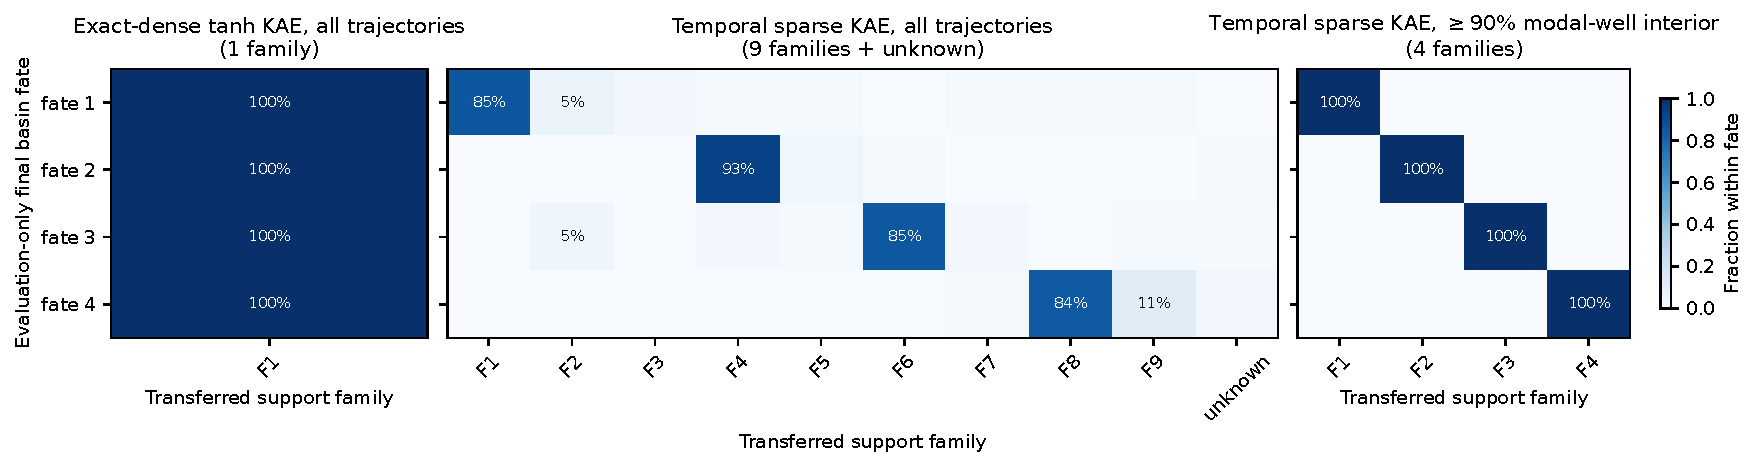
\includegraphics[width=\textwidth]{figures/neurips_paper_2026/fig_allen_cahn_support_contingency.pdf}
\caption{Row-normalized final-state fate--support contingency for the fixed
display seed on the new-simulation-seed Allen--Cahn holdout. Exact dense assigns every
fate to one family (left). Temporal sparse has one dominant family per fate on
all trajectories but additional families in mixed-domain fields (center). On
the single-well-dominated final-field slice prospectively frozen for this new
holdout after earlier mixed-domain fragmentation, it transfers exactly
four families in one-to-one correspondence with the four finite-time
modal-well fates (right). Aggregate claims use all ten
model seeds, not this display seed alone. Columns preserve the raw
training-codebook family IDs in numeric order, independent of evaluation fate;
row labels give panel-specific trajectory counts;
the center and right panels share one family axis, so blank right-panel columns
are families absent from the declared slice.}
\label{fig:allen_cahn_support_contingency}
\end{figure*}

Forecasts are evaluated at physical times $0.1,0.5,1,2,4,8,12,16,20$, so
the display does not rely on a nominally multi-step but physically negligible
horizon. Temporal sparse has lower error than dense through time $4$, but the
ordering reverses at time $8$ and remains reversed. At time $20$, direct,
dense, and sign-support final field MSE are $0.0293$, $0.1184$, and
$0.2991$; their final RMSE ratios to persistence are $0.218$, $0.442$, and
$0.649$. All three learned rows beat persistence, but the direct control is
best. This separates the high-dimensional sparse forecasting claim, which
comes from Lorenz--96 and the separate packet below, from this physics-based
multibasin representation claim. The temporal-support model's pre-split group
activity is nearly complete, so it is not evidence of intrinsic coefficient
sparsity before its sign split.

\paragraph{Separate forecast-optimized global-$K$ packet.}
This experiment shares the $d_x=512,d_z=2{,}048$, grid, stored interval, and
four-well system, but it is a different trained model and dataset split. It
uses 512 training trajectories, full 200-step sequences, batch size 8, 2,000
autoencoder-pretraining updates, and 3,500 forecast-training updates. Adam has
learning rate $3\times10^{-4}$ for the network and $10^{-6}$ for $K$, with
zero weight decay. The selected soft-thresholded recipe uses shrinkage $0.15$, ordinary
elementwise sparsity weight $0.01$, and zero temporal-group penalty. The dense
arm uses tanh hidden activations, a linear latent output, a full trainable $K$,
and zero sparsity, shrinkage, dropout, weight decay, transition, or block
penalties; all ten fail-closed audits pass. An exact checkpoint audit finds
the same trainable tensor shapes/count and shared convolutional, decoder, and
$K$ backbone, with $12{,}698{,}690$ trainable parameter entries in both arms.
The nominal $2{,}048^2$ LISTA recurrence matrix stays exactly zero and is inert
with one LISTA loop, leaving $8{,}504{,}386$ effective forward-path parameters
per arm. Thus the treatment is jointly soft-thresholding at $0.15$ and an
$L_1$ weight of $0.01$ under matched parameter count and backbone, not equal
function-class capacity or an isolated component test.

Selection used a three-seed, four-recipe development screen. The selected
recipe was then trained for seeds 64--73 and scored on 256 fresh initial
conditions from simulation seed $20{,}260{,}724$, using no basin label or
count. Checkpointing used the even development partition and joint H160/H200
endpoints; held-out scoring uses all fresh validation trajectories and no
checkpoint reselection. Forecasting is direct
repeated-$K$ rollout without re-encoding. Mean near-zero fraction at threshold
$10^{-3}$ is $0.434$ for sparse and $0.0025$ for dense. All 20 runs are finite;
mean active A100L utilization is $95.55\%$ (range $90.56$--$96.78\%$).
On the opened development screen, the one-pass soft-thresholded sparse arm had lower through-horizon mean
and terminal MSE than its same-recipe dense arm in all 16 comparisons across
the four forecast-weighting/latent-consistency recipes. This is descriptive
screen robustness, not confirmation or a threshold-versus-$L_1$ ablation.

\begin{table}[tbp]
\centering
\caption{Separate forecast-optimized Allen--Cahn comparison. ``Mean'' averages
field MSE over every forecast state through the horizon; it is not an
unnormalized cumulative sum. Intervals resample paired model seeds. The
one-sided max-$t$ values are a multiplicity sensitivity, not a replacement for
the failed internally frozen four-cell gate.}
\label{tab:allen_cahn_global_k_forecast_optimized}
\resizebox{\textwidth}{!}{\begin{tabular}{llrrrrl}
\toprule
Horizon & Endpoint & Dense & Sparse & Reduction & Wins & Marginal 95\% CI; max-$t$ $p$ \\
\midrule
H160 & Mean through H & 0.04503 & 0.04220 & 6.3\% & 8/10 & [2.6, 9.5]\%; 0.014 \\
H160 & Terminal & 0.05189 & 0.05065 & 2.4\% & 7/10 & [-1.6, 6.0]\%; 0.197 \\
H200 & Mean through H & 0.04731 & 0.04472 & 5.5\% & 8/10 & [1.7, 8.8]\%; 0.019 \\
H200 & Terminal & 0.06086 & 0.05890 & 3.2\% & 7/10 & [-0.8, 6.7]\%; 0.112 \\
\midrule
\multicolumn{7}{l}{\footnotesize Matched trainable tensor shapes and effective forward-path parameter count; sparse jointly applies soft-thresholding $0.15$ and $L_1$ weight $0.01$.} \\
\multicolumn{7}{l}{\footnotesize Internally frozen confirmation gate: failed; sealed holdout not generated or opened.} \\
\bottomrule
\end{tabular}
}
\end{table}

At H160, sparse/dense through-horizon mean field MSE is
$0.04220/0.04503$; at H200 it is $0.04472/0.04731$. These are reductions of
$6.30\%$ and $5.48\%$, each with 8/10 paired wins. Terminal reductions are
$2.38\%$ and $3.22\%$, each with 7/10 wins and an interval crossing zero.
The corresponding through-horizon MSE ratios to persistence are
$0.0958/0.1023$ at H160 and $0.0938/0.0993$ at H200 for sparse/dense;
terminal ratios are $0.0824/0.0844$ and $0.0937/0.0968$. Thus the physical
times 16--20 are nontrivial relative to persistence even though the terminal
sparse--dense effect remains uncertain.
The rule frozen before fresh confirmation-data generation required all four
mean and terminal cells to pass; it failed.
In addition to both terminal intervals crossing zero, H200 terminal misses the
minimum $5\%$ reduction and 8/10-win criteria.
The conditional seed-$20{,}260{,}725$ holdout was never generated or opened.

\paragraph{Same-checkpoint new-initial-condition robustness check.}
After the preceding four-cell decision failed, we prospectively froze the
already positive H200 through-horizon endpoint. This endpoint choice was
outcome-aware. We crossed the same ten sparse and ten dense checkpoints with
three newly generated datasets (simulation seeds $1{,}775{,}404{,}171$,
$74{,}732{,}421$, and $293{,}789{,}188$), each containing 256 trajectories.
There was no retraining, checkpoint reselection, periodic re-encoding, label
use, or basin-count use. The rollout encodes once and applies the unchanged
global $K$ for 200 steps, reaching physical time 20. Datasets are averaged
within each paired model seed before inference, so the inferential unit remains
the ten paired checkpoint seeds rather than the 30 crossed seed--dataset cells.

Sparse/dense through-horizon field MSE is $0.04616/0.04903$, a $5.86\%$
reduction with 8/10 paired-seed wins. A 100,000-resample paired-seed bootstrap
interval is $[2.40\%,9.21\%]$ and the exact one-sided paired sign-flip value is
$9/1{,}024=0.00879$. Dataset-specific reductions are $4.68\%$, $5.88\%$, and
$7.03\%$, all in the same direction; these three values are descriptive rather
than independent hypothesis tests. H200 terminal error is descriptive only:
$0.06476/0.06683$, a $3.09\%$ reduction with 7/10 wins. A separate authenticated
recomputation exactly reproduced all primary values and authenticated the
complete 60-cell roster, all 20 checkpoints, and all three datasets. The
result establishes same-checkpoint robustness to new initial conditions in
this fixed PDE condition. It does not retroactively repair the original
four-cell gate or establish terminal, parameter, resolution, physics, or
system generalization. Descriptively, across the full physical-time trace, the
sparse arm-mean instantaneous MSE is lower at all 200 times, but the
running-mean reduction declines from about 14\% early to 5.86\% at $T=20$.
Over the late half, $T=10.1$--20, sparse/dense instantaneous means are
$0.05216/0.05380$, only a $3.06\%$ reduction; no simultaneous curve-wide
inference is claimed. The result remains a
trajectory-average rather than terminal or asymptotic advantage. H200 equals
the trained temporal horizon and is not extrapolation beyond it.

\begin{figure*}[tbp]
\centering
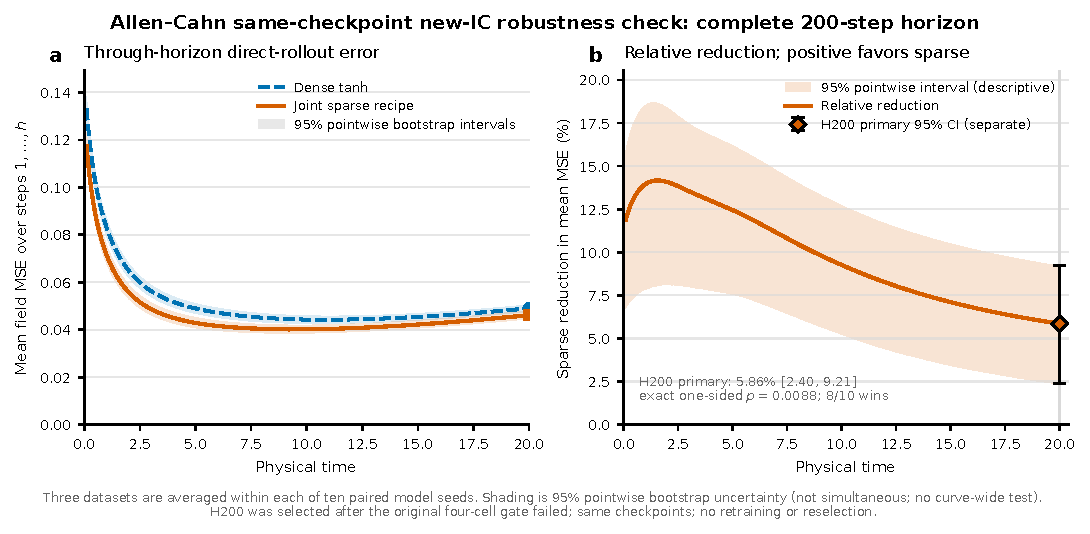
\includegraphics[width=\textwidth]{figures/neurips_paper_2026/fig_allen_cahn_new_ic_replication_full_horizon.pdf}
\caption{Complete 200-step Allen--Cahn same-checkpoint new-initial-condition
robustness trace. H200 was selected after the original four-cell gate failed;
the checkpoints were neither retrained nor reselected.
The left panel reports mean field MSE over steps $1,\ldots,h$ against physical
time. The right panel reports the ratio-of-arm-means reduction. Shading is a
descriptive pointwise 95\% paired-seed bootstrap band and is neither
simultaneous nor a curve-wide test; the black H200 interval is the separate
100,000-resample primary interval. Datasets are averaged within each of ten
paired model seeds.}
\label{fig:allen_cahn_new_ic_full_horizon}
\end{figure*}

\paragraph{Outcome-aware physical concordance on the same forecasts.}
On the identical 20 checkpoints, three datasets, 256 trajectories per dataset,
and 200-step direct rollouts, sparse is directionally better at the H200
cumulative endpoint on all seven frozen secondary metrics. Pixel nearest-well
disagreement, well-area total-variation error, interface-edge disagreement,
full-free-energy error, and gradient-energy error fall by
$4.61\%$, $6.07\%$, $2.25\%$, $6.20\%$, and $8.58\%$, respectively, and
survive Holm correction across all seven metrics. Modal-well accuracy rises by
$0.236$ percentage points and potential-energy error falls by $3.77\%$, but
their Holm-adjusted values are $0.303$ and $0.119$ and their intervals include
zero. Thus the result is broad phase-assignment, interface, and thermodynamic
concordance, not seven statistically significant endpoints.

Every metric was frozen and computed for every trajectory and time. Pixel and
modal-well scores use the four known wells only for evaluation; well-area error
compares the four phase fractions; interface error compares periodic nearest-
well boundary indicators; and the energy terms use the discrete Lyapunov
functional whose derivative matches the pinned reaction--diffusion generator.
Datasets are first averaged within model seed, leaving ten paired checkpoint
seeds as the inferential units. Exact one-sided paired sign flips are Holm-
adjusted as one seven-metric family, and intervals resample paired seeds. No
periodic re-encoding, fate label, basin count, finite-prefix filtering, or
trajectory exclusion alters a forecast.

\begin{table*}[t]
\centering
\small
\caption{Outcome-aware, same-checkpoint secondary Allen--Cahn analysis showing all seven frozen metrics at the H200 cumulative endpoint. Effects are relative reductions for the six lower-is-better errors and percentage-point differences for modal accuracy. Confidence intervals are paired-seed 95\% intervals for the oriented absolute effect; $q$ is Holm-adjusted across all seven metrics. Bold $q$ values are at most 0.05.}
\label{tab:allen_cahn_physics_metrics}
\begin{tabular}{lrrrrr}
\toprule
Metric & Dense & Sparse & Oriented effect & Wins & Holm $q$ / abs. 95\% CI \\
\midrule
Pixel phase error & 0.09424 & 0.08990 & 4.61\% & 9/10 & \textbf{0.0146} / [0.00229, 0.00610] \\
Modal-well accuracy & 0.90742 & 0.90977 & +0.236 pp & 5/10 & 0.3027 / [-0.00551, 0.01061] \\
Well-area TV error & 0.05402 & 0.05074 & 6.07\% & 8/10 & \textbf{0.0352} / [0.00112, 0.00535] \\
Interface-edge error & 0.09966 & 0.09742 & 2.25\% & 9/10 & \textbf{0.0146} / [0.00118, 0.00311] \\
Free-energy error & 0.02843 & 0.02667 & 6.20\% & 10/10 & \textbf{0.0068} / [0.00112, 0.00243] \\
Potential-energy error & 0.03597 & 0.03462 & 3.77\% & 8/10 & 0.1191 / [-0.00006, 0.00311] \\
Gradient-energy error & 0.02897 & 0.02649 & 8.58\% & 10/10 & \textbf{0.0068} / [0.00164, 0.00332] \\
\bottomrule
\end{tabular}
\end{table*}


\begin{figure*}[tbp]
\centering
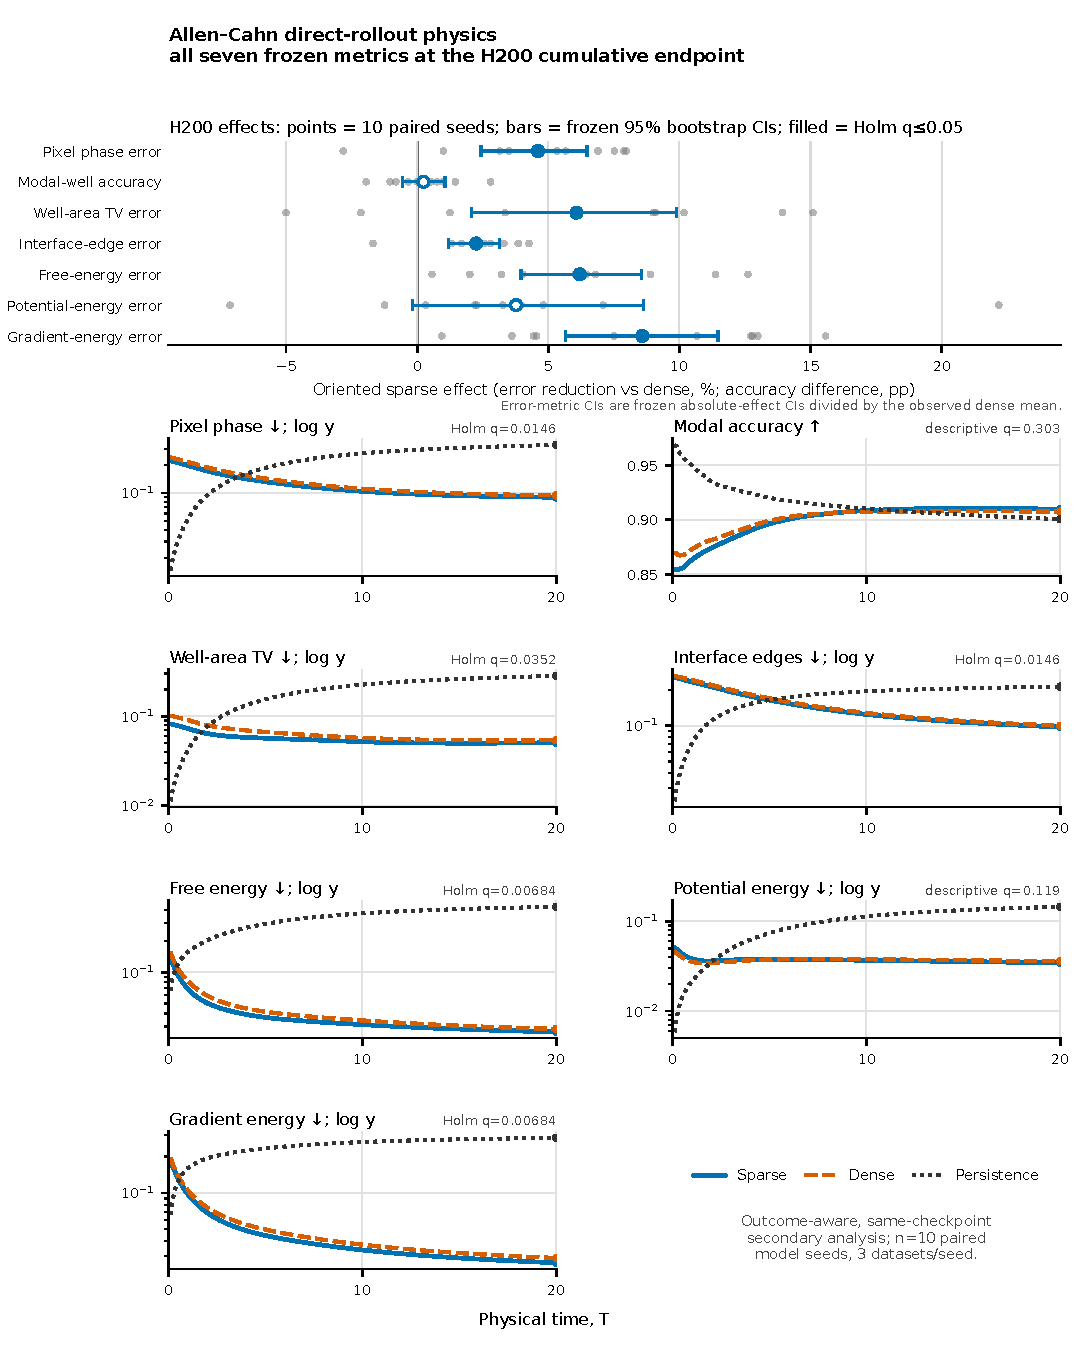
\includegraphics[width=0.94\textwidth]{figures/neurips_paper_2026/fig_allen_cahn_physics_metrics.pdf}
\caption{All seven frozen Allen--Cahn physical metrics on the same-checkpoint
new-initial-condition forecasts. The top panel shows the H200 cumulative
oriented effect, all paired-seed effects, and paired-seed intervals; filled
marks survive seven-way Holm correction. Lower panels show every arm-mean
curve through physical time 20, including persistence. Curves are descriptive;
the statistical family consists of the seven H200 cumulative endpoints. The
analysis is outcome-aware because H200 and these checkpoints were retained
after the original four-cell forecasting gate failed.}
\label{fig:allen_cahn_physics_metrics}
\end{figure*}

This translation addresses whether lower field MSE merely reflects benign
amplitude changes: the favorable interface and separated potential/gradient
energy components argue against that narrow explanation in this condition.
It does not identify a sparse component as causal, repair the original gate,
establish terminal superiority, or generalize over retraining, PDE parameters,
grid resolution, or another physical system. The appropriate next experiment
is therefore a prospectively frozen recipe across new physical conditions,
not additional tuning on the already opened condition.

\paragraph{Historical hard-system negative.}
A separate 15-seed stress test used $d_z=1{,}024$, sequence length 8, batch
size 256, and 100,000 updates on 15-dimensional fixed eight-basin competitive
Lotka--Volterra, Hopfield $N=P=16$, and identical-frequency ring Kuramoto
$N=16$. Under each row's evaluation-selected best periodic-reencoding
cadence, the tanh/no-output-gate Dense MLP beat every sparse/LISTA recipe on
all three systems at H100, H500, and H1000. At H1000 its system-median MSEs
were $0.2999/2.8034/7.7872$, versus $0.3210/8.3277/15.5167$ for the closest
LISTA-SB row. All arms used AdamW weight decay $10^{-4}$; activation,
iterative-encoder, block-$K$, capacity, and learning-rate differences preclude
a sparsity-only attribution. This is a mandatory negative stress test and
rules out a universal sparse forecasting advantage.

\paragraph{Requested half-global/half-local diagnostic.}
At one separate seed (61), a sequence-80 sign-split model received 2,000
autoencoder and 1,750 shared-$K$ updates, followed by 1,750 updates to either
full route-local $2{,}048\times2{,}048$ matrices or a matched continued-global
branch. Every support and cosine-cluster local recipe selected its zero-update
initialization. At H200, local/global through-horizon mean MSE is
$0.07871/0.06463$ (local 21.8\% worse), terminal MSE is $0.12048/0.10168$
(18.5\% worse), and route coverage is $0.840<0.90$. Full matrices rule out
insufficient rank as the sole explanation, but this one-seed near-dense
ancestor (pre-split activity $0.9982$) differs from the positive global recipe;
the result falsifies this routing recipe, not all local-$K$ methods.

\begin{figure*}[tbp]
\centering
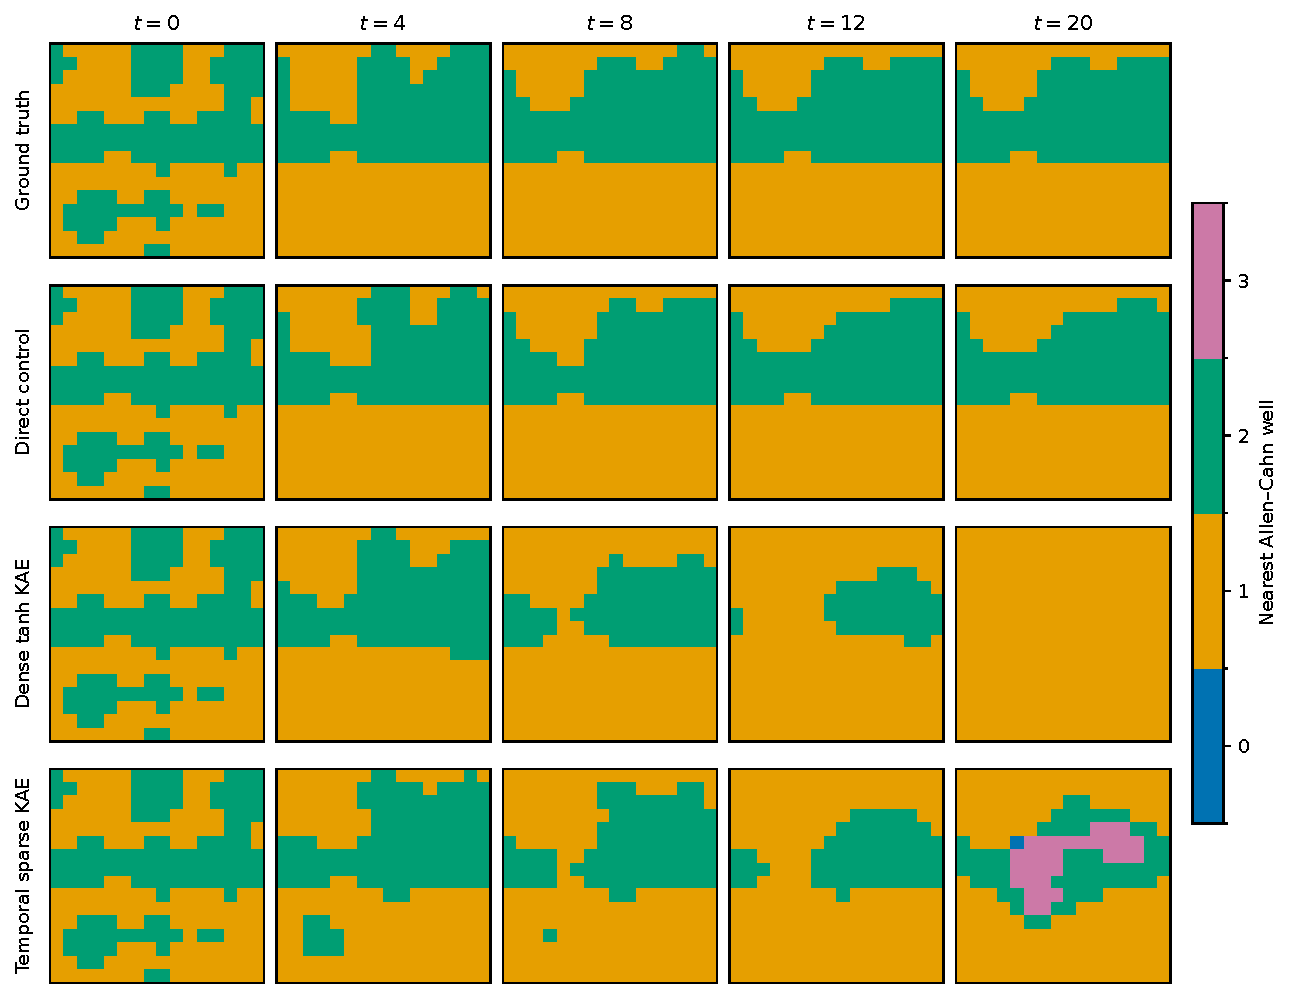
\includegraphics[width=\textwidth]{figures/neurips_paper_2026/fig_allen_cahn_time20_snapshots.pdf}
\caption{Predeclared qualitative long-horizon Allen--Cahn trajectory on the
new-simulation-seed holdout, shown as nearest-well maps at physical times through
$20$. The direct control preserves the evolving interface most faithfully;
the sign-split temporal-support KAE has the weakest long-horizon forecast. The trajectory
and model seed were fixed before the new holdout was opened and are not used
for quantitative selection.}
\label{fig:allen_cahn_time20_snapshots}
\end{figure*}

\paragraph{Inference.}
The Lorenz--96, Allen--Cahn temporal-support, forecast-optimized Allen--Cahn,
same-checkpoint new-IC, and secondary physical-metric packets average trajectories within model seed and use ten paired
model-initialization seeds as inferential units. Lorenz--96 and temporal-support
intervals use 100,000 percentile bootstrap resamples; their paired tests
enumerate all sign flips, with long-horizon $p$-values Holm-adjusted within each
declared family. The forecast-optimized packet instead uses 50,000 paired-seed
resamples of each ratio-of-arm-means reduction. Its four intervals are marginal
and its frozen primary decision is an intersection-union gate; the exact
one-sided 1,024-swap max-$t$ calculation is a multiplicity sensitivity over the
dependent H160/H200 mean/terminal cells (H160 is a prefix of H200), not a
replacement decision. Lorenz--96 and the original Allen--Cahn intervals
condition on one fixed evaluation dataset. The new-IC interval averages three
fixed datasets within each paired checkpoint seed. They quantify variation
across the ten trained seed pairs, but not an independent repeat of the
training/selection pipeline, a future retraining packet, PDE parameters,
resolutions, or physical systems. The new-IC
check crosses the three datasets with every checkpoint, averages them within
paired model seed, uses 100,000
paired-seed resamples, and enumerates the same 1,024 paired sign flips. Neither benchmark uses fate labels, basin counts, or
trajectory assignments for training, encoding, representative fitting, or
family transfer. In the temporal-support packet, validation fate metrics select
the T20 scope, Jaccard-0.40 rule, temporal weight, and advancement of the whole
fixed ten-seed packet; labels on the
new-simulation-seed holdout only score the frozen assignments and the
declared single-well-dominated final-field slice.
The physical-metric packet uses the same within-seed dataset averaging and
100,000 paired-seed resamples, one-sided exact sign flips, and Holm correction
over all seven H200 cumulative endpoints. Its two nonsignificant metrics and
all terminal and late-window summaries remain visible rather than being
removed from the family.

\clearpage

\section{Support-projected one-step leakage of one global operator}
\label{app:global_k_support_closure}

This diagnostic tests a narrow mechanism hypothesis: a single learned global
operator can act approximately within several support-selected coordinate
sets on observed projected codes even when no basin label, basin count, or
trajectory-to-basin assignment is used.
It does not train local operators. In the implementation's row-vector
convention, a family mask defines a diagonal projector \(P_f\) and the learned
prediction is \(z_{t+1}=z_tK\). Cross-support output is therefore
\(z_tP_fK(I-P_f)\). This is the transpose-equivalent of
\((I-P_f)KP_fz_t\) in the paper's column-vector convention.

\paragraph{Existence construction.}
One matrix is not mathematically incompatible with several local laws. For
row-form affine dynamics $x^+=xA_b+c_b$, let
$\psi_b(x)=[x,1]$ and
$K_b=\left[\begin{smallmatrix}A_b&0\\c_b&1\end{smallmatrix}\right]$.
In an overcomplete direct-sum lift, set $K=\operatorname{diag}(K_1,\ldots,K_B)$
and let a routed basin-interior encoder place $\psi_b(x)$ only in block $b$. If $P_b$ selects that
block, then $P_bK(I-P_b)=0$ and $zP_bK^h=zK^h$, while different restrictions
contain different laws; a block-aware decoder recovers the physical state.
Unused blocks mean the architecture need not be told the realized basin count.
This proves an algebraic interior-chart possibility with a block-aware decoder,
not a continuous global encoder across basin boundaries, learned discovery,
label-free routing, or realization by our checkpoints.

\paragraph{Protocol frozen before evaluation.}
The roster contains unstructured signed sparse encoders with full
\(256\times256\) learned matrices: three initialization seeds on each of the
15 two-dimensional controlled systems. Their sign-split ReLU output
mechanically permits at most one active coefficient per positive/negative
pair, so the result concerns the learned sign-split coordinate basis rather
than generic sparse encoders. For every checkpoint, 128 newly generated trajectories
are split 64/64 by whole trajectory. The first half alone forms support
families using \(\lvert z_i\rvert>10^{-3}\), greedy Jaccard-0.50 merging, and a
minimum of 128 fit transitions per retained family. The second half alone is
scored. The primary slice contains transitions whose current and next support
masks both map to the same retained family. This future-conditioned
persistence criterion makes the closure test easier and is an important scope
restriction. The authenticated evaluator also emitted an all-current regime
before execution, without conditioning on the next support. Its reduction was
performed post hoc as a no-next-state guard and is not a second frozen
decision. Eligibility requires
at least two retained families, current/persistent coverage of at least
\(0.80/0.70\), and at least 64 scored transitions per reported family.

The activity leakage diagnostic is
\(\lVert zP_fK(I-P_f)\rVert/\lVert zP_fK\rVert\); its matrix-wide analogue is
\(\lVert P_fK(I-P_f)\rVert_F/\lVert P_fK\rVert_F\). To exclude the trivial case
where \(K\approx I\), change-normalized versions instead use
\(\lVert zP_f(K-I)\rVert\) and \(\lVert P_f(K-I)\rVert_F\) in their denominators.
We also report the inside-support residual of the
post-hoc restricted predictor \(P_fKP_f\), the encoded next-state energy
outside the current support, and the residual of the unmodified global \(K\)
relative to identity. The restricted predictor is an evaluation diagnostic,
not a retrained model. Finally, pairwise symmetric normalized Frobenius
distance between restricted operators tests whether the selected coordinate sets have
more differentiated restrictions than a matched null.

The null uses 16 coordinate permutations frozen in advance. Each permutation
moves positive/negative sign partners together and is applied jointly to
codes, next codes, masks, and projectors while leaving \(K\) fixed. It
therefore preserves norms, support cardinality, activity, and sign-split
semantics while breaking alignment with the learned operator. Metrics reduce
first within a run, then by the median across eligible seeds within each
system, and finally by the median across eligible systems; transitions are not
treated as independent replicates.

\begin{table}[tbp]
\centering
\caption{Held-out one-step support-closure diagnostics for one unchanged
global \(K\). The table reports both the post-hoc reduction of the
pre-execution evaluator-emitted all-current guard and the internally frozen
persistent-family primary. The matched null permutes sign pairs while holding
\(K\) fixed. The frozen branch is labeled partial closure, but its failed
differentiation guard permits only a lower-leakage claim.}
\label{tab:global_k_support_closure}
\resizebox{\textwidth}{!}{\begin{tabular}{llrrrrl}
\toprule
Slice & Diagnostic & Observed & Matched null & Obs./null & Wins & Gate \\
\midrule
All-current guard$^{\dagger}$ & Raw-$K$ activity leakage & 0.0047 & 0.2065 & 0.022 & 15/15 & Ref. pass \\
 & Raw-$K$ matrix Frobenius leakage & 0.0538 & 0.2080 & 0.240 & 15/15 & Diagnostic \\
 & $(K-I)$-normalized leakage & 0.3382 & 0.7830 & 0.433 & 15/15 & Ref. pass \\
 & $(K-I)$ matrix Frobenius leakage & 0.5541 & 0.7834 & 0.699 & 15/15 & Diagnostic \\
 & Post-hoc $PKP$ inside residual & 0.0100 & 0.1646 & 0.053 & 15/15 & Ref. pass \\
 & Restricted-operator distance & 0.9741 & 0.9830 & 0.993 & 0/15 & \textbf{Ref. fail} \\
\midrule
Persistent primary & Raw-$K$ activity leakage & 0.0047 & 0.2065 & 0.022 & 15/15 & Pass \\
 & Raw-$K$ matrix Frobenius leakage & 0.0538 & 0.2080 & 0.240 & 15/15 & Diagnostic \\
 & $(K-I)$-normalized leakage & 0.3394 & 0.7831 & 0.435 & 15/15 & Pass \\
 & $(K-I)$ matrix Frobenius leakage & 0.5539 & 0.7834 & 0.699 & 15/15 & Diagnostic \\
 & Post-hoc $PKP$ inside residual & 0.0100 & 0.1646 & 0.053 & 15/15 & Pass \\
 & Restricted-operator distance & 0.9741 & 0.9830 & 0.993 & -- & \textbf{Fail} \\
\midrule
\multicolumn{7}{l}{\footnotesize $^\dagger$Post-hoc reduction of a pre-execution evaluator-emitted no-next-state guard; not a second frozen decision.} \\
\multicolumn{7}{l}{\footnotesize The guard adds only 3,527 transitions (0.96 percentage points); medians are over system-level seed medians.} \\
\multicolumn{7}{l}{\footnotesize Frozen primary decision: partial closure; the differentiation guard fails; $PKP$ is a post-hoc restriction.} \\
\bottomrule
\end{tabular}
}
\end{table}

\begin{table}[tbp]
\centering
\caption{Triggered exact-dense specificity control. Dense tanh models use
zero weight decay and no sparsity-producing mechanism. At every matched
physical state, the dense projector selects the top-magnitude coordinates
with exactly the corresponding sparse support cardinality. Values are
observed/permutation-null ratios; the last column is sparse/dense. The
source-locked reducer retains 41/45 dense runs and 14 systems, versus 45/45
runs and 15 systems for sparse; its pre-outcome two-eligible-seed rule was
omitted from the card. Sparse-to-dense ratios of observed/null activity and
residual are 0.039/0.108 on the 14 common systems, 0.040/0.109 under the literal-card all-15 rule, and 0.041/0.110
when all three seeds are required (12 systems).}
\label{tab:global_k_dense_specificity}
\resizebox{0.82\textwidth}{!}{\begin{tabular}{lrrr}
\toprule
Metric & Sparse / null & Dense / null & Sparse / dense \\
\midrule
Raw-$K$ activity leakage / null & 0.022 & 0.567 & 0.039 \\
Post-hoc restricted residual / null & 0.053 & 0.486 & 0.108 \\
\bottomrule
\end{tabular}
}
\end{table}

\begin{figure*}[tbp]
\centering
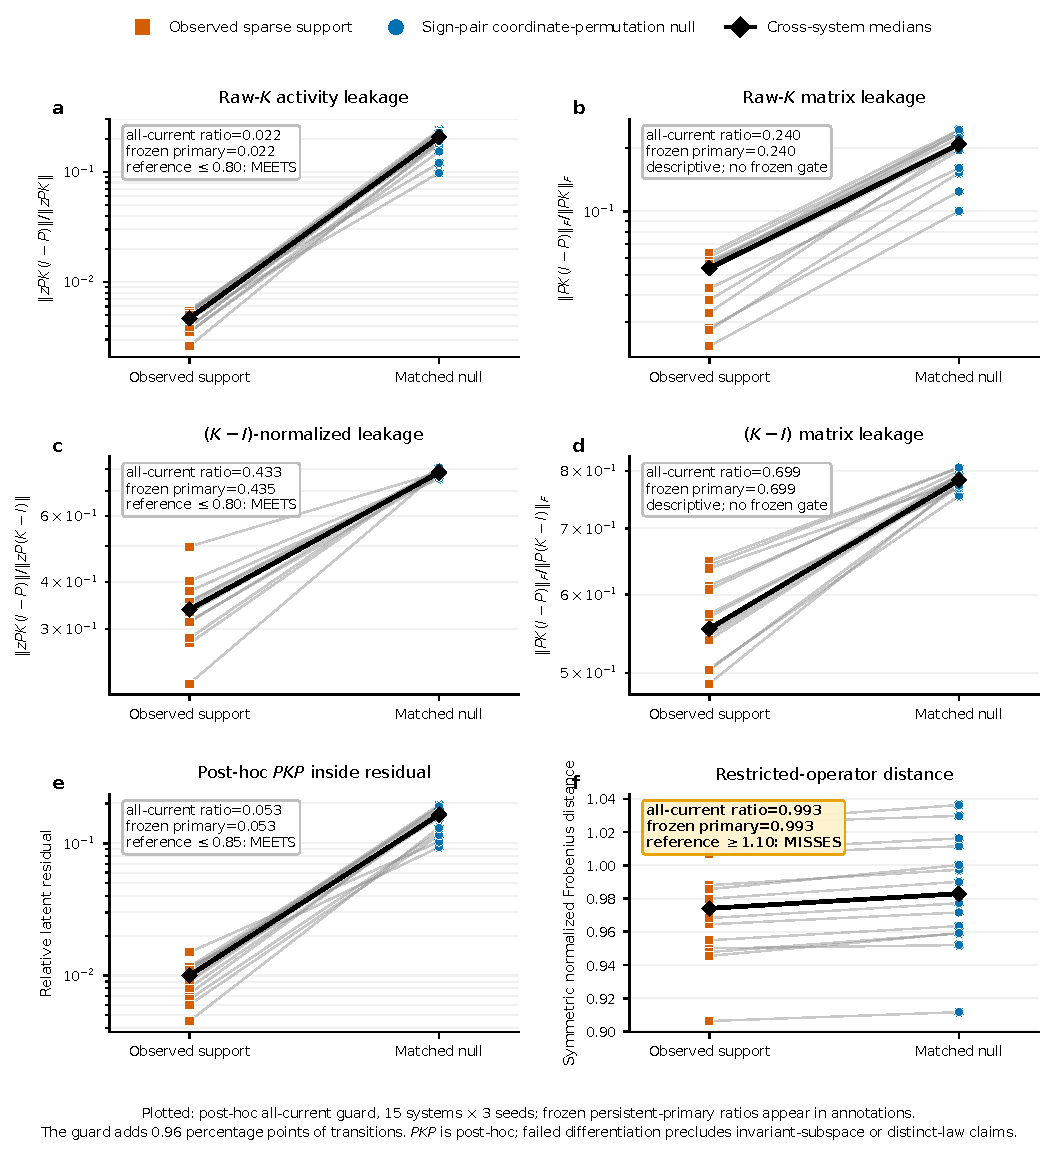
\includegraphics[width=\textwidth]{figures/neurips_paper_2026/global_k_support_closure_paired_systems.pdf}
\caption{System-level seed medians for the no-next-state all-current guard;
annotations give its ratio and the internally frozen persistent-primary ratio.
Lower is better in the first five panels. The two matrix-wide panels are
descriptive diagnostics without retrofitted decision thresholds.
Restricted-operator differentiation
is null-like and fails its reference threshold.}
\label{fig:global_k_support_closure}
\end{figure*}

All 45 runs and all 15 systems are eligible. Mean current and persistent
coverage are \(0.963\) and \(0.953\). Retained families average 5.84 per run,
their representatives average 95.0 of 256 coordinates, and the projected
source captures 0.997 of source-code RMS energy. At the system-median level,
the all-current observed/null activity leakage is \(0.0047/0.2065\) (ratio
\(0.022\)); change-normalized leakage is \(0.338/0.783\) (ratio \(0.433\));
the corresponding matrix-wide values are \(0.0538/0.2080\) (ratio \(0.240\))
and \(0.554/0.783\) (ratio \(0.699\)); and restricted inside-support residual
is \(0.0100/0.1646\) (ratio \(0.053\)). All 15 systems favor the observed masks
on each of these five diagnostics. Their ratios are numerically close to the
frozen persistent-primary values \(0.022/0.240/0.435/0.699/0.053\). Removing
the next-family condition therefore leaves the aggregate essentially
unchanged on this high-persistence sample. Because the guard adds only 3,527
transitions, or 0.96 percentage points, it does not determine behavior on
boundary-switching transitions. The unmodified
global-\(K\) residual is 0.583 times identity on the all-current guard.

The frozen strong decision nevertheless fails: restricted-operator distance
is \(0.974\) for observed supports and \(0.983\) under the null, a ratio of
\(0.993\) rather than the required \(1.10\). Thus support-projected one-step
leakage is lower than under matched permutations in this learned sign-split
basis, but the result does not establish distinct local laws, exact invariant subspaces, a direct-sum
decomposition, decoded forecasting, or Allen--Cahn behavior. Because the
result is basis-dependent, the frozen protocol triggered a
cardinality-matched exact-dense tanh specificity control.

That control is complete. Across the 45-run dense roster, 41 runs and 14
systems meet the source-locked reducer's eligibility rule. Sparse/dense
observed-to-null ratios are $0.039$ for raw-$K$ activity leakage and
$0.108$ for the post-hoc $P_fKP_f$ residual, far below both frozen $0.90$
gates; all 14 common eligible systems favor sparse on both metrics. The
reducer's requirement of at least two eligible seeds per system existed before
outcomes but was omitted from the prediction card, so it is not described as
card-preregistered; the frozen headline also aggregates 15 sparse versus 14
dense systems. Common-14 sensitivities are $0.039/0.108$, literal-card
minimum-one-seed all-15 sensitivities are $0.040/0.109$, and an all-three-seed
12-system sensitivity is $0.041/0.110$, so the conclusion is nearly unchanged
under these population choices. Thus the low support-projected one-step leakage
is specific to the complete sparse recipe relative to cardinality-matched
dense tanh top-$k$ coordinate masks. Dense masks have no natural dense-support semantics, and
encoder/decoder parameterization and optimization differ; this is a
complete-recipe specificity control, not a sparsity-only causal ablation,
basis-invariant result, distinct-law test, or forecasting comparison.

\paragraph{Prospective physical-law test.}
A separate frozen test trained ten new paired sparse/dense models on a
controlled two-dimensional system with three basin-specific laws. Training
and support-family discovery used neither basin labels nor the basin count;
evaluation labels only matched discovered families to the benchmark laws.
The authenticated result is negative. Only 24/30 sparse seed--basin rows
passed the prespecified differentiability gate, leaving 6/10 complete sparse
seeds rather than the required 8/10. On those rows, the Jacobian of the actual
restricted predictor selected the correct law in 9/24 nearest-law comparisons,
passed its ratio gate in 4/24, its affine gate in 2/24, and its finite-radius
gate in 0/24. The isolated $K$-induced update component was descriptively
nearest to the correct law in 24/24 rows and met projected-code closure in
23/24, but its aggregate matched-null guard failed (null won 6/10 seeds;
$p=0.377$). Dense specificity was invalid because only six pairs were jointly
differentiable. The isolated-component diagnostic is therefore stronger than
the actual-predictor diagnostic, but it also fails its aggregate null and the
packet fails validity. This contrast motivates testing reconstruction geometry
without identifying it as the cause and supports no multiple-law,
invariant-subspace, or sparse-superiority claim.

A final frozen recursive residual-routing diagnostic used one unchanged $K$
but did not yield a scientific decision: five of ten seed shards completed, a
sixth encountered a nonfinite payload value (\texttt{inf}) during strict serialization, four were
not run, and the required telemetry assessment and summary were absent. Under
its exact-ten fail-closed protocol, every forecasting claim tier is
invalid at the frozen validity tier and directionally unadjudicated; no partial
shard was inspected and the execution is not evidence for or against the hypothesis.

\section{Additional background}
\label{app:background}

\subsection{Koopman operators and finite-dimensional approximations}
\label{app:koopman_background}

Consider the stored-step map used in \cref{sec:problem},
\begin{equation}
  x_{k+1}=F_{\Delta t}(x_k), \qquad x_k\in\mathcal X\subseteq\R^{d_x}.
\end{equation}
Koopman operator theory studies the evolution of observables rather than the evolution of the state directly. An observable is a measurement function \(g:\mathcal X\to\R\), and the Koopman operator \(\mathcal K\) acts by composition:
\begin{equation}
  (\mathcal K g)(x)=g(F_{\Delta t}(x)).
\end{equation}
The map \(F_{\Delta t}\) may be nonlinear, but \(\mathcal K\) is linear on the function space of observables. If a finite vector of observables
\begin{equation}
  \Phi(x)=\big[g_1(x),\ldots,g_{d_z}(x)\big]^\top
\end{equation}
spans a Koopman-invariant subspace, then there is a matrix \(K\in\R^{d_z\times d_z}\) such that
\begin{equation}
  \Phi(x_{k+1})=\Phi(F_{\Delta t}(x_k))=\mathcal K\Phi(x_k)=K\Phi(x_k).
\end{equation}
In that case the nonlinear dynamics are exactly linear in the observable coordinates \(z_k=\Phi(x_k)\). Learning Koopman models can therefore be viewed as searching for observables whose span is invariant enough to support useful finite-dimensional linear prediction.

In practice, the infinite-dimensional operator is approximated from data. Given snapshot pairs \(\{(x_k,x_{k+1})\}\) and a chosen feature map \(\Phi\), dynamic mode decomposition and extended dynamic mode decomposition (eDMD) estimate a finite transition by least squares \citep{schmid_dmd_2010,rowley_2009_spectral,tu_dynamic_2014,williams_datadriven_2015,williams_kernel-based_2016}:
\begin{equation}
  K
  =
  \argmin_{\widetilde K\in\R^{d_z\times d_z}}
  \sum_k \norm{\Phi(x_{k+1})-\widetilde K\Phi(x_k)}_2^2.
\end{equation}
DMD is the special case \(\Phi(x)=x\), so it fits a linear state-space surrogate without a learned nonlinear lift. eDMD extends this by choosing a richer observable dictionary. Koopman autoencoders replace the fixed observable dictionary with a learned encoder and decoder, which is the setting used in this paper.

\subsection{Why multibasin systems may benefit from local structure}
\label{app:multibasin_background}

Near appropriate attracting sets, classical linearization and Koopman eigenfunction constructions can produce useful local or basin-restricted coordinates. Global results are more restrictive: multi-attractor systems should not in general be assumed to admit one exact finite-dimensional linearization with a continuous, state-reconstructing encoder--decoder pair \citep{lan_linearization_2013,brunton_koopman_2016,pan_lifting_2024,liu_properties_2025}. These results motivate local structure, but they do not prove that every learned global KAE must fail or that sparse supports recover the theoretical local coordinates.

For the present paper, a learned finite-dimensional KAE is treated as an approximation. Sparse supports provide one possible discrete and inspectable key: a support may index a basin part or local predictive chart while coefficient values carry within-chart information. Whether that interpretation holds is an empirical question tested by the transductive alignment and staged forecasting experiments.

\subsection{Koopman autoencoders and periodic re-encoding}
\label{app:kae_reencoding_background}

A standard Koopman autoencoder learns an encoder \(\Enc:\R^{d_x}\to\R^{d_z}\), decoder \(\Dec:\R^{d_z}\to\R^{d_x}\), and latent transition \(K\) so that
\begin{equation}
  z_k=\Enc(x_k),\qquad z_{k+1}\approx Kz_k,\qquad x_k\approx\Dec(z_k).
\end{equation}
A schematic one-step objective has the form
\begin{equation}
  \min_{\Enc,\Dec,K}
  \sum_k
  \norm{x_k-\Dec(\Enc(x_k))}_2^2
  +
  \lambda_{\rm lin}
  \norm{\Enc(x_{k+1})-K\Enc(x_k)}_2^2 .
  \label{eq:KAE-standard-objective}
\end{equation}
This objective is useful as a reference point, but it is not sufficient for the present study. It does not directly train decoded multi-step rollouts, does not impose a sparse support object, and does not test whether the support itself selects a useful local predictive rule. The training objective in \cref{sec:method_training} therefore keeps the autoencoding and latent-linearity terms but adds decoded rollout prediction over windows, sparsity on the rolled latent states, and optional transition-structure penalties.

Periodic re-encoding interrupts a latent rollout after a fixed number of stored observation steps. For period \(m\),
\begin{equation}
  \tilde z_{k+m}=K^m z_k,\qquad
  \tilde x_{k+m}=\Dec(\tilde z_{k+m}),\qquad
  z_{k+m}=\Enc(\tilde x_{k+m}).
\end{equation}
This is the same mechanism defined in \cref{eq:reencode}. It uses only the model's own predicted state and is therefore not a teacher-forced correction. The point is to refresh the latent embedding and, in sparse models, to refresh the support as the predicted state moves through regions where a different local linear description may be more appropriate \citep{fathi2024course}.

\subsection{Sparse coding and LISTA}
\label{app:sparse_lista_background}

Classical sparse coding seeks a code \(z\) that reconstructs a signal from a small set of active dictionary atoms:
\begin{equation}
  z^\star(x)=
  \argmin_{z\in\R^{d_z}}\;\frac{1}{2}\norm{x-Dz}_2^2+\lambda_{\rm sc}\norm{z}_1,
  \qquad \lambda_{\rm sc}>0,
\end{equation}
where \(D\) is a dictionary and \(\lambda_{\rm sc}\) controls sparsity \citep{olshausen_emergence_1996,chen_atomic_1998,donoho_optimally_2003}. For a fixed dictionary, and under the usual uniqueness and non-boundary conditions for the Lasso solution, the active set and signs are locally constant over regions of the input space, while the coefficient values vary continuously within a fixed active set. The decoder reconstruction then lies in the span of the selected dictionary columns, giving a union-of-subspaces geometry. Each exact support can index a local chart, and the greedy Jaccard procedure in \cref{sec:method_supports} groups nearby Boolean support vectors into support families when threshold noise or boundary effects fragment the exact masks.

LISTA replaces an iterative sparse-coding solver with a learned finite-depth shrinkage network \citep{gregor_learning_2010}. In the notation of \cref{eq:lista}, the encoder forms a pre-code from the input and repeatedly applies learned affine refinement followed by soft thresholding. In this paper, the encoder is trained jointly with the Koopman rollout objective rather than solving the sparse-coding problem at evaluation time. Thresholding turns the latent into continuous coefficients plus an explicit support. The experiments ask whether absolute-threshold support families align transductively with evaluation-only native or nearest-center-proxy labels and whether a separately fitted training-distribution family partition can route useful local affine predictors.

\clearpage
\section{Preliminary coauthor checklist}
\label{app:checklist_details}
\begingroup
\sloppy
\paragraph{Status.}
This is a factual pre-submission record for coauthor review, not the official
venue questionnaire.  Application of the final venue style determines the
official question set, numbering, and response format; these answers must then
be reconciled with that form.  Nothing here asserts that a public artifact,
anonymous URL, DOI, or release has been completed.
\paragraph{Claims and evidence.}
The manuscript makes three bounded empirical claims: sparse KAE rows improve
forecasting over the reported Dense MLP KAE rows; LISTA support families align
transductively with evaluation-only native or nearest-center-proxy labels on a
controlled high center-margin slice;
and a staged training-distribution support-family route has descriptively lower
controlled-forecasting error than a same-budget global-\(K\) LISTA baseline
under an optimistic asymmetric selector.  The paper states no new theorem
or proof, no exact global linearization, and no out-of-sample basin-discovery
guarantee.  Benchmark definitions and training/evaluation protocols are in
\cref{app:controlled_inventory,app:dysts_inventory_full,app:experimental_details};
support construction and inference are in
\cref{app:support_definitions,app:statistical_testing}.
\paragraph{Limits on interpretation.}
\begin{itemize}
  \item Best-periodic cadence is chosen on the test trajectories, and the MSE
  reducer omits nonfinite steps, so finite prefixes of divergent rollouts can
  contribute.
  \item Alignment fits families on all states in each evaluation trajectory
  collection.  Two gated systems use native labels and centers; the other
  \(13\) use deterministic endpoint-estimated centers at the known benchmark
  count and nearest-center proxy labels.  Scoring retains states at or above
  each label's \(75\)th center-margin percentile, including ties, so it need
  not retain exactly one quarter; Triple-well Duffing retains all \(16{,}512\)
  states.  This margin need not equal true basin-boundary distance.  Labels
  and centers select only the scored subset, label sample counts are not
  equalized, and the reported family count includes only family IDs observed
  on that subset.  Conditional entropy uses natural logarithms and is reported
  in nats.  The result is transductive and two-dimensional; alignment uses
  Jaccard threshold \(0.50\), while the separate staged route uses \(0.40\).
  \item The staged route-fit packet has \(512\) configured rows but only
  \(256\) unique trajectories because one batch is duplicated exactly.  Its
  checkpoint selector uses the first \(32/100\) reported starts, while the
  global baseline uses a distinct \(16\)-start, H200 final-error selector.
  Thus the \(225\) nested system--seed comparisons are optimistic and
  descriptive, not a clean held-out or causal comparison.
  \item Standalone controls use three seeds and unmatched trajectories; the
  intervention covers one checkpoint.
  \item LISTA decoders are atom-normalized whereas MLP decoders are not.
  Dysts LISTA--SB is a same-budget two-loop/sign-split ablation, unlike the
  one-loop/ReLU LISTA and LISTA--BD rows. Structured-transition rows use a known
  controlled-benchmark basin count or a hand-set Dysts lobe/scroll/equilibrium
  count only to set the number of blocks.
\end{itemize}
\paragraph{Reproducibility and access status.}
The working repository contains explicit controlled-system vector fields,
benchmark adapters, training and evaluation code, seeds, locked dependencies,
tests, manuscript sources, and paper-facing aggregate artifacts.  Controlled
trajectories are regenerable from the explicit analytic or piecewise-analytic
systems; Dysts trajectories are
regenerable from the documented package and cache protocol.  Exact model,
metric, split, cadence, support, and standalone-control recipes are recorded in
\cref{app:experimental_details,app:support_definitions}.  Bitwise equality
across GPU models and numerical-library versions is not claimed.  No verified
public anonymous archive or DOI is identified in the manuscript, so open
code/data availability is currently answered \emph{No}.
\paragraph{Compute accounting.}
The following are conservative SLURM allocation ceilings, not measured
consumption or energy estimates:
\begin{itemize}
  \item Controlled training comprises \(15\times6\times15=1350\) runs, each
  requesting one cluster-assigned GPU, four CPU cores, \(16\) GB host memory,
  and at most \(24\) hours: at most \(32{,}400\) GPU-hours and \(129{,}600\)
  allocated CPU-core-hours.
  \item Dysts training comprises \(10\times6\times15=900\) runs packed up to
  \(12\) per allocation, with one GPU, four CPU cores, \(16\) GB, and at most
  \(72\) hours per full pack: at most \(5{,}400\) GPU-hours and \(21{,}600\)
  allocated CPU-core-hours.
  \item The staged routing packet comprises \(15\times15=225\) runs, each
  requesting one GPU, four CPU cores, \(24\) GB, and at most three hours: at
  most \(675\) GPU-hours and \(2{,}700\) allocated CPU-core-hours.
  \item Retained Dysts cache/evaluation jobs add approximately \(4{,}700\)
  CPU-core-hours; controlled support diagnostics add approximately \(290\)
  CPU-core-hours; the one-checkpoint intervention allocation adds at most
  \(3\) GPU-hours.
\end{itemize}
The GPU model was scheduler-assigned and is therefore unspecified.  These
ceilings exclude superseded historical packets and can substantially exceed
actual use because jobs may finish early and packed runs share allocations.
\paragraph{Assets, attribution, and licenses.}
The controlled benchmark contains \(15\) author-retained analytic or
piecewise-analytic systems.
Claude Opus 4.5 assisted system ideation; human authors audited the retained
definitions and metadata before their experimental use.  The LLM is not part
of model training, rollout, routing, metric computation, or statistical
testing.  LLM assistance also contributed to manuscript and checklist editing;
the authors remain responsible for the equations, protocols, and numerical
claims.
The external benchmark uses right-hand sides and metadata from
\texttt{dysts} \(0.96\), with project-generated standardized trajectories, and
the manuscript cites the associated Gilpin papers.  Local package metadata is
not sufficient to state a definitive redistribution license: it contains an
MIT license classifier but a bundled Apache-2.0 license text.  The authoritative
Dysts license and any system-level attribution requirements therefore remain
unresolved.  The repository itself has a top-level MIT license, but no public
artifact or separate license for generated benchmark definitions, figures,
tables, caches, or checkpoints is claimed here.
\paragraph{Ethics, human subjects, and broader impact.}
The experiments use simulated dynamical-system states and public benchmark
definitions, with no participants, crowdworkers, personal data, private
records, or human-generated labels.  Human-subject review, consent,
compensation, and IRB approval are therefore not applicable.  This is
methodological forecasting research, not a validated safety-critical control
system.  Learned support families can be misread as physical or causal regimes,
and failures near boundaries, in additional high-dimensional systems, or on
empirical data could be consequential; downstream use requires independent
validation and safeguards.
\endgroup


\bibliographystyle{plainnat}
\bibliography{neurips_sparse_koopman_multibasin}

\end{document}
